%% thesis.tex — 경북대학교 박사학위논문 메인 파일
%% XeLaTeX + kotex 환경
%% 컴파일: xelatex thesis && bibtex thesis && xelatex thesis && xelatex thesis

\documentclass[11pt]{knuthesis}

%% ============================================================
%% 패키지 로드
%% ============================================================

%% 수학
\usepackage{amsmath,amssymb,mathrsfs}

%% 그래픽
\usepackage{graphicx}
\graphicspath{{figures/}{../mutbench/}{../../results/mutbench/}{../../docs/figures/}}

%% 표
\usepackage{booktabs}
\usepackage{tabularx}
\usepackage{multirow}
\usepackage{longtable}
\usepackage{array}

%% 알고리즘
\usepackage[ruled,vlined,linesnumbered]{algorithm2e}

%% 코드
\usepackage{listings}
\lstset{
  basicstyle=\ttfamily\small,
  breaklines=true,
  frame=single,
  numbers=left,
  numberstyle=\tiny,
}

%% 참고문헌 (natbib + bibtex)
\usepackage[numbers,sort&compress]{natbib}
\bibliographystyle{unsrtnat}

%% 하이퍼링크
\usepackage[pdfencoding=auto,colorlinks=true,linkcolor=blue,citecolor=blue,urlcolor=blue]{hyperref}
\usepackage{bookmark}

%% 기타
\usepackage{enumitem}
\usepackage{xcolor}
\usepackage{subcaption}
\usepackage{url}

%% ============================================================
%% 줄간격 (1.85)
%% ============================================================
\setstretch{1.85}

%% ============================================================
%% 폰트 설정
%% ============================================================
\usepackage{fontspec}
\setmainfont{TeX Gyre Termes}
\setmainhangulfont{Noto Serif CJK KR}[
  BoldFont=Noto Serif CJK KR Bold,
]
\setsanshangulfont{Noto Sans CJK KR}[
  BoldFont=Noto Sans CJK KR Bold,
]

%% ============================================================
%% 저자 정보
%% ============================================================
\title{Systematic Benchmarking and Adaptive Clustering Frameworks\\for Multi-Scale Genomic Data Analysis}
\ktitle{다층적 게놈 데이터 분석을 위한\\체계적 벤치마킹과 적응형 클러스터링 프레임워크}
\author{Hwijun Kwon}
\kauthor{권 휘 준}
\advisor{Inuk Jung}
\kadvisor{정 인 욱}
\major{School of Computer Science and Engineering}
\kmajor{컴퓨터학부}
\degreedate{2026}{8}

%% 심사위원 (추후 수정)
\committeechairman{OOO}
\committeememberA{OOO}
\committeememberB{OOO}
\committeememberC{OOO}
\committeememberD{OOO}

%% ============================================================
%% 문서 시작
%% ============================================================
\begin{document}

%% ----------------------------------------------------------
%% 전면부 (Front Matter)
%% ----------------------------------------------------------
\pagenumbering{roman}

%% 겉표지
\makecoverpage

%% 속표지
\makeinnertitle

%% 인준지
\makeapprovalpage

%% 감사의 글
\makeacknowledgments{%
  % 감사의 글
먼저 학위 과정 전반에 걸쳐 세심한 지도와 아낌없는 격려를 보내주신 정인욱 지도교수님께 깊은 감사를 드립니다.
교수님의 학문적 통찰과 인내심 있는 가르침이 없었다면 본 연구는 완성될 수 없었습니다.

바쁘신 중에도 논문 심사를 맡아주시고 귀중한 조언을 해주신 심사위원 교수님들께도 진심으로 감사드립니다.

함께 연구하며 많은 도움을 준 연구실 동료들에게도 감사의 마음을 전합니다.
특히 MOSD 연구를 함께 수행한 한은용 연구원, MutClust 연구에 함께 참여한 윤소현, 정다빈 연구원께 감사드립니다.

마지막으로, 긴 학위 과정 동안 항상 곁에서 응원해준 가족에게 깊은 감사와 사랑을 전합니다.

\vspace{2em}
\hfill 2026년 8월

\hfill 권 휘 준

}

%% 한글 초록
\makekorabstract{%
  % 한글 초록
\begin{sloppypar}
바이러스 게놈의 변이 핫스팟 탐지는 변이주 감시와 백신 설계에 필수적이나, 탐지 방법론을 체계적으로 비교·평가할 수 있는 벤치마크 프레임워크가 부재하였다.
기존 연구들은 단일 병원체·단일 탐지 방법에 의존하여, 어떤 점수화(scoring)와 탐지(detection) 조합이 어떤 병원체에 적합한지 알 수 없었다.

본 연구에서는 이 문제를 해결하기 위해 MutBench를 제안한다.
MutBench는 변이 핫스팟 탐지를 위한 최초의 체계적 벤치마크 프레임워크로, 세 가지 핵심 구성요소를 포함한다:
(1)~같은 바이러스 종 내에서 서로 다른 계통에서 독립적으로 반복 출현한 수렴 진화 위치를 양성 선택 기준(Layer~A),
정화 선택 하의 보존 구조 영역을 음성 기준(Layer~B),
Deep Mutational Scanning(DMS) 실험적 적합도 데이터를
기능적 검증(Layer~C)으로 통합하는 3층 ground truth 체계,
(2) $\text{hotspot-score} = (\text{recall} + \text{precision} + \text{stability}) / 3$으로 정의되는 복합 평가 지표,
(3) Stage~1에서 SARS-CoV-2에 대한 심층 분석, Stage~2에서 11개 병원체에 대한 8{,}580회 평가(20개 점수화 공식 $\times$ 39개 탐지 알고리즘 $\times$ 11개 병원체)를 수행하는 2단계 실험 설계이다.

Stage~1에서는 MutClust-Hybrid가 최고 hotspot-score(0.778)를 달성하여,
도메인 특화 사전지식과 데이터 기반 클러스터링의 결합이 효과적임을 확인하였다.
Stage~2의 11개 병원체 대규모 벤치마크에서는 점수화(scoring) 방법과 병원체 간 상호작용이 전체 성능 분산의 29.6\%를 설명하여 최대 분산 원천으로 확인되었다($\omega^2_{\text{scoring} \times \text{pathogen}} = 0.296$). 이는 탐지 알고리즘 패밀리 주효과($\omega^2 = 0.013$)의 22배로, ``어떤 알고리즘을 쓰느냐''보다 ``어떤 생물학적 정보를 쓰느냐''가 성능을 결정하는 핵심 요인임을 입증한다.
Friedman 검정($\chi^2 = 7.69$, $p = 0.990$)에서 상위 20개 조합 간 유의한 차이가 없음을 확인하였으며, LOPO 교차검증에서 11개 병원체 모두 서로 다른 최적 조합을 보였다(일반화 성공률 0/11).

이러한 결과는 최적 탐지 전략이 병원체에 따라 근본적으로 상이하며, 단일 고정 방법이 아닌 병원체별 적응적 접근이 필요함을 통계적으로 입증한다.
6개 정보 카테고리(빈도 기반, MSA 유래, 계통 분석, 구조 기반, AI 기반, 복합)에 걸친 20개 점수화 유형 분석에서 9가지 서로 다른 최적 scoring이 관찰되었다: FUBAR 계통선택 점수(H3N2), 호모플래시(Norovirus), 단백질 언어모델(SARS-CoV-2, RSV), 의미적 변화(EV-A71), 안정성 예측(Rabies), 빈도 기반(HCV, Influenza B, MERS).
또한 탐지된 핫스팟이 실험적으로 확인된 백신 escape 위치와 4.90배 enrichment($p < 0.0001$)를 보여, 공중보건 감시에 대한 실용적 가치를 입증하였다.
다중 정보 통합이 실험적 탐색 범위를 축소함을 확인하였다(H3N2 백신 escape enrichment 4.012배, $p = 0.0023$).

\vspace{1em}
\end{sloppypar}
\noindent\textbf{주요어}: 변이 핫스팟 탐지, 벤치마크 프레임워크, 바이러스 게놈, 복합 평가 지표, 다중 정보 통합 분석, SARS-CoV-2, Deep Mutational Scanning

}

%% 목차
\setcounter{page}{1}
\tableofcontents
\clearpage

%% 표목차
\listoftables
\clearpage

%% 그림목차
\listoffigures
\clearpage

%% ----------------------------------------------------------
%% 본문 (Main Matter)
%% ----------------------------------------------------------
\pagenumbering{arabic}
\setstretch{1.85}

% Chapter 1: Introduction
\chapter{서론}
\label{ch:introduction}

\section{연구 배경}
\label{sec:intro_background}

2019년 말 출현한 SARS-CoV-2는 전 세계적으로 7억 건 이상의 확진 사례를 발생시키며, 바이러스 유전체 분석의 중요성을 재확인시켰다~\cite{harvey2021tracking}.
바이러스는 복제 과정에서 지속적으로 변이를 축적하며, 특정 유전체 위치에 변이가 집중되는 현상을 hotspot이라 한다.
Hotspot은 전파력 증가, 면역 회피(immune evasion, 기존 면역 반응을 피하는 능력), 약물 저항성 등 바이러스의 주요 표현형 변화와 직접 관련되므로, 이를 정확히 검출하는 것은 백신 설계, 항바이러스제 개발, 실시간 유전체 감시의 핵심 과제이다~\cite{youn2025mutclust,nextstrain2018hadfield,rambaut2020pangolin}.

그러나 바이러스 변이 hotspot 검출 방법들의 성능을 체계적으로 비교·평가할 수 있는 벤치마크 프레임워크가 확립된 바 없다. 형식적으로, 바이러스 단백질 서열의 다중 서열 정렬(MSA)이 주어졌을 때, 검출 과제는 통계적으로 유의하게 높은 변이율을 보이는 유전체 위치의 부분집합을 식별하는 것이다. 그러나 표준화된 ground truth, 복합 평가 지표, 교차 병원체 검증 방법론이 존재하지 않으며, 이는 암 유전체학의 부분적 벤치마킹~\cite{bailey2018comprehensive}에도 불구하고 마찬가지이다.
본 연구자는 이전에 다중 오믹스 통합을 위한 체계적 벤치마크 프레임워크(MOSD~\cite{han2025mosd})와 적응적 hotspot 검출 알고리즘(MutClust~\cite{youn2025mutclust})을 개발하였으며, 정량적 평가 프레임워크 없이 MutClust를 개발한 경험이 본 연구의 직접적 동기가 되었다.

Nextstrain~\cite{nextstrain2018hadfield}이나 PANGO 계통 분류~\cite{rambaut2020pangolin}와 같은 현행 바이러스 유전체 플랫폼은 변이체 출현을 모니터링하지만, hotspot 검출 방법의 체계적 평가를 제공하지 않는다.
표준화된 벤치마크의 부재는 방법 개발자가 자신의 접근법을 객관적으로 비교할 수 없고, 최종 사용자가 특정 병원체에 어떤 방법을 적용할지 정보에 기반한 선택을 할 수 없음을 의미한다.


\section{연구 동기 및 문제 정의}
\label{sec:intro_motivation}

바이러스 변이 hotspot 검출의 체계적 평가가 부재함으로 인해, 다음과 같은 세 가지 구체적 문제가 발생한다.

첫째, \textbf{표준화된 평가 프레임워크의 부재}이다.
MutClust를 포함한 기존 hotspot 검출 방법들은 각자의 데이터셋과 평가 기준을 사용하여 성능을 보고하므로, 방법 간 공정한 비교가 불가능하다.
MutClust의 유일한 검증 수단인 bootstrap 검정은 검출된 클러스터의 통계적 유의성만을 확인하는 자기 참조적 방법으로, 해당 클러스터가 생물학적으로 의미 있는 기능적 영역에 대응하는지는 검증할 수 없다.

둘째, \textbf{독립적 ground truth에 기반한 검증의 부재}이다.
Hotspot 검출 결과를 객관적으로 평가하려면 알고리즘과 독립적인 정답 기준이 필요하나, 바이러스 유전체학에서 이러한 ground truth 체계가 정의된 사례가 없다.
수렴 진화(convergent evolution, 독립적 계통에서 동일 위치에 반복적으로 발생하는 변이) 위치, 정제 선택(purifying selection, 해로운 변이를 제거하는 자연선택) 위치, Deep Mutational Scanning(DMS, 단백질의 모든 가능한 단일 아미노산 변이의 기능적 영향을 실험적으로 측정하는 기술) 데이터 등 활용 가능한 독립적 증거원이 존재함에도 체계적으로 통합되지 않았다.

셋째, \textbf{최적 방법의 병원체 의존성에 대한 경험적 증거의 부재}이다.
기존 방법들은 단일 병원체에 맞추어 조정된 매개변수를 사용하며, 그 일반화 가능성이 통계적으로 확립되지 않았다.
병원체별 유전체 특성(길이, 변이율, 재조합 빈도 등)의 차이가 최적 검출 전략에 체계적 영향을 미치는지는 검증되지 않았다.
이것은 알고리즘 선택 문제(algorithm selection problem)~\cite{rice1976algorithm}의 구체적 사례이다: 특정 게놈 특성을 가진 병원체가 주어졌을 때, 어떤 탐지 방법을 적용해야 하는가? 체계적인 교차 병원체 평가 없이는 이 질문에 답할 수 없다.


\section{연구 목적}
\label{sec:intro_objectives}

위의 문제를 해결하기 위하여, 본 연구는 다음 두 가지 목표를 설정한다.

\begin{enumerate}[label=\textbf{목표 \arabic*.}]
  \item \textbf{바이러스 변이 hotspot 검출을 위한 체계적 벤치마크 프레임워크(MutBench)의 구축}: 3계층 ground truth(수렴 진화 기반 양성, 정제 선택 기반 음성, DMS 기능적 적합도), hotspot-score $= (\text{recall} + \text{precision} + \text{stability}) / 3$ (여기서 stability는 부분추출 반복 시 탐지 결과의 재현성을 측정한다) 복합 평가 지표, 2단계 실험 설계(1단계: SARS-CoV-2 심층 분석, 2단계: 9종 RNA 바이러스 $\times$ 9가지 스코어링 $\times$ 39개 탐지 방법, 총 3,159개 평가)를 포함하는 벤치마크 프레임워크를 구축한다.

  \item \textbf{병원체 적응적 방법 선택의 필요성에 대한 경험적 입증}: 대규모 벤치마크 결과에 대한 통계 분석(ANOVA, Friedman 검정, LOPO 교차 검증)을 통해, 단일 최적 방법이라는 전제가 병원체 전반에 걸쳐 성립하지 않음을 경험적으로 확립하고, PAHD 프레임워크의 개념 증명 프로토타입을 제시한다(제~\ref{ch:results}장 참조).
\end{enumerate}


\section{연구 기여}
\label{sec:intro_contributions}

본 연구의 학술적 기여는 다음과 같다.

\textbf{기여 1. MutBench 벤치마크 프레임워크.}
MutBench는 바이러스 변이 hotspot 검출을 위한 최초의 체계적 벤치마킹 프레임워크이다.
수렴 진화 위치를 양성 기준(Layer~A), 정제 선택 위치를 음성 기준(Layer~B), DMS 실험 데이터를 기능적 적합도 기준(Layer~C)으로 활용하는 3계층 ground truth 체계를 정의하였다.
정확도(recall, precision)와 신뢰성(stability)을 동시에 평가하는 hotspot-score 복합 지표를 도입하고, SARS-CoV-2 심층 분석과 9종 병원체 대규모 비교를 결합하는 2단계 실험 설계를 제시하였다.

\textbf{기여 2. 병원체 적응적 방법 선택 필요성의 통계적 입증.}
9종 RNA 바이러스에 대한 평가 결과, 9개 병원체 모두 상이한 최적 조합을 보이며(LOPO 교차 검증 0/9 일치), 방법 계열과 병원체 간 상호작용이 ANOVA에서 최대 분산 원천이었다.
Friedman 검정은 방법 간 성능 순위가 병원체에 따라 체계적으로 달라짐을 확인하였다.
이 결과는 단일 최적 방법이라는 전제가 성립하지 않음을 확립하며, PAHD 프레임워크의 개념 증명 프로토타입을 제시한다(상세 통계는 제~\ref{ch:results}장 참조).


\section{논문 구성}
\label{sec:intro_organization}

본 학위논문은 6개의 장으로 구성된다.

\textbf{제~\ref{ch:background}장, 관련 연구}에서는 바이러스 변이 hotspot 검출에 관한 기존 문헌을 조사하고, MutClust~\cite{youn2025mutclust}의 핵심 방법론 및 MutBench 개발의 동기가 된 한계점을 요약한다.

\textbf{제~\ref{ch:mutbench}장, 자료 및 방법}에서는 본 학위논문의 핵심 기여인 MutBench 벤치마크 프레임워크의 자료와 방법론을 상세히 기술한다.
제3.1절은 자료(대상 병원체, ground truth 체계, DMS 데이터)를 기술한다. 제3.2--3.4절은 방법을 제시한다: 제3.2절은 MutClust 변형 및 hotspot-score 지표를 포함하는 벤치마크 프레임워크 설계, 제3.3절은 스코어링 공식과 탐지 방법 계열, 제3.4절은 평가 지표 및 통계 분석 설계를 다룬다.

\textbf{제~\ref{ch:results}장, 실험 결과}에서는 실험 결과를 네 개 절로 구분하여 보고한다: 단일 병원체 벤치마크(합성 데이터 비교, 다중 ground truth 평가, 실제 GISAID 검증, SARS-CoV-2에 대한 외부 방법 비교), 견고성 검증(통계적 검증, 민감도 분석, 시간적 일반화, indel 제외), 교차 병원체 검증(H3N2 검증, 3D 구조 분석, 계통발생학적 시뮬레이션, ESM-2 교차 패러다임 검증), 9-병원체 대규모 벤치마크(ANOVA, Friedman 검정, LOPO 교차 검증, PAHD 개념 증명 프로토타입).

\textbf{제~\ref{ch:discussion}장, 논의}에서는 실험 결과의 종합적 해석, MutBench의 방법론적 함의, 한계점, 그리고 PAHD 개념적 프레임워크의 향후 방향을 논의한다.

\textbf{제~\ref{ch:conclusion}장, 결론}에서는 연구의 기여를 요약하고, 한계점을 분석하며, 향후 연구 방향을 제시한다.


% Chapter 2: Background and Prior Work (Unified)
% Combines: literature review + MOSD summary + MutClust summary
\chapter{배경 및 선행 연구}
\label{ch:background}

본 장에서는 본 학위논문의 핵심 연구인 MutBench를 이해하기 위한 배경을 네 개의 절로 구성하여 제시한다.

먼저, 다중오믹스 통합 분석(Section~\ref{sec:bg_moi})과 바이러스 변이 핫스팟 탐지(Section~\ref{sec:bg_hotspot})에 관한 선행 연구를 고찰한다.
이 두 분야는 본 학위논문의 핵심 연구(MutBench)와 선행 연구(MOSD, MutClust)가 다루는 핵심 영역이며, 공통적으로 클러스터링 기반 방법에 의존하면서도 체계적 벤치마킹이 부족하다는 문제를 공유한다.

이어서, 본 학위논문의 선행 연구로서 출판된 두 논문---MOSD (Section~\ref{sec:mosd_summary})와 MutClust (Section~\ref{sec:mutclust_summary})---를 요약한다.
MOSD는 다중오믹스 통합을 위한 체계적 벤치마킹 방법론을 확립하였고, MutClust는 바이러스 변이 핫스팟 탐지를 위한 적응형 알고리즘을 개발하였다.
본 장에서는 이 두 연구의 성과와 한계를 모두 제시하여, MutBench 개발의 동기와 방법론적 기반을 명확히 한다.


%% ===================================================================
%%  SECTION 1: 다중오믹스 통합 분석
%% ===================================================================
\section{다중오믹스 통합 분석}
\label{sec:bg_moi}

\label{subsec:bg_moi_methods}
\label{subsec:bg_benchmarking}

Multi-Omics Integration (MOI)은 유전자 발현, DNA 메틸화, 복제수 변이 등 다층적 생물학적 데이터를 결합하여 복잡한 질병의 분자적 특성을 포괄적으로 규명하기 위한 접근법이다.
그래프 기반(SNF~\cite{wang2014snf}, NEMO~\cite{rappoport2018nemo}), 행렬 분해 기반(MOFA~\cite{argelaguet2018mofa}, iClusterPlus~\cite{shen2013iclusterplus}), 합의 기반(COCA~\cite{hoadley2014coca}, PINSPlus~\cite{nguyen2017pinsplus}) 등 다양한 MOI 방법이 개발되었으나, 어떤 조건에서 어떤 방법이 최적인지에 대한 근본적 질문이 남아 있었으며, 기존 벤치마크 연구들~\cite{chauvel2020sample, rappoport2018benchmark, pierrejean2020feature, tini2019multi, duan2021evaluation}은 각각 1--3개의 요인만을 독립적으로 조사하여 통합적 가이드라인을 제공하지 못하였다.
저자는 이 공백을 해결하기 위해 MOSD 프레임워크~\cite{han2025mosd}를 개발하여, 10개 TCGA 암종에 걸쳐 10개 MOI 방법에 대한 9개 요인의 영향을 체계적으로 평가하였다.
MOSD는 두 가지 핵심 설계 원칙을 도입하였다: 세 가지 상보적 클러스터링 지표를 동등 가중치로 결합한 복합 평가 지표(cluster-score)와, 평가 대상 요인만 변동시키고 나머지를 통제하는 단일 요인 분리 설계이다.
Weber et al.~\cite{weber2019benchmarking}은 엄격한 벤치마킹에 중립적 평가, 다중 지표, 통제된 실험 설계, 재현성이 필요함을 제시하였으며, MOSD는 이러한 원칙을 MOI에 구현하였다. 이와 동일한 설계 원칙이 바이러스 핫스팟 탐지를 위한 MutBench로 이전되며, 이는 Section~\ref{sec:mosd_summary}에서 상술한다.


%% ===================================================================
%%  SECTION 2: 바이러스 변이 핫스팟 탐지
%% ===================================================================
\section{바이러스 변이 핫스팟 탐지}
\label{sec:bg_hotspot}

\subsection{변이 핫스팟 탐지 방법론}
\label{subsec:bg_hotspot_methods}

변이 핫스팟은 유전체 내에서 변이가 비균일적으로 집중되는 영역으로, 구조적 또는 면역학적 선택압 하에 있는 기능적으로 중요한 부위를 반영할 가능성이 높다.
바이러스 유전체에서 핫스팟을 식별하는 것은 변이체 출현 예측, 백신 표적 선정, 치료제 개발에 핵심적이다.
기존의 핫스팟 탐지 접근법은 빈도 기반, 엔트로피 기반, 밀도 기반 방법으로 분류할 수 있다.

\textbf{빈도 기반 접근법}은 아미노산 또는 뉴클레오타이드 수준에서 변이 빈도를 계산하고, 높은 빈도를 보이는 위치를 핫스팟으로 지정한다.
직관적이고 구현이 용이하지만, 두 가지 근본적 한계를 지닌다.
첫째, \textbf{계통 편향(lineage bias)}: 특정 계통이 데이터베이스에서 과대 대표될 경우 해당 계통의 정의 변이가 불균형적으로 높은 빈도 점수를 받는다.
D614G와 같이 거의 모든 현대 SARS-CoV-2 서열에서 관찰되는 변이는 실제 적응도 이점을 반영하지만, 근고정(near-fixation) 속도는 초기 팬데믹의 창시자 효과에 의해 증폭되어, 빈도 데이터만으로는 선택과 유전적 부동의 상대적 기여를 구분하기 어렵다.
둘째, \textbf{희귀 변이의 간과}: 낮은 빈도로 발생하지만 다양한 형태로 나타나는 변이---면역 회피 또는 바이러스 적응을 시사할 수 있는---가 체계적으로 간과된다.

\textbf{엔트로피 기반 접근법}은 Shannon entropy를 사용하여 주어진 위치에서 뉴클레오타이드 다양성을 측정한다.
Mullick et al.~\cite{mullick2021entropy}은 Shannon entropy와 K-means clustering을 결합하여 SARS-CoV-2 Spike 단백질의 핫스팟을 탐지하였다.
그러나 기존의 뉴클레오타이드 엔트로피는 변이 발생 여부와 관계없이 모든 뉴클레오타이드의 분포를 반영하므로, 변이 발생을 조건으로 한 실효적 다양성을 포착하지 못한다.
또한 K-means clustering은 클러스터 수를 사전에 지정해야 하며 밀도 구조를 고려하지 않는다.

\textbf{암 유전체학 방법.}
암 유전체학에서는 체세포 변이의 핫스팟을 탐지하기 위한 다양한 방법이 개발되었다.
MutSigCV~\cite{lawrence2013mutsigcv}는 배경 변이율을 모델링하여 과도한 변이를 보이는 유전자를 식별하나, 유전자 수준의 해상도에서 작동한다.
OncodriveCLUST~\cite{tamborero2013oncodriveclust}는 변이의 위치적 클러스터링 편향을 무작위 기대값과 비교한다.
HotMAPS~\cite{tokheim2016hotmaps}는 변이를 3D 단백질 구조에 매핑하여 공간적 핫스팟을 탐지하나, 단백질 구조 데이터가 필요하며 코딩 영역에 제한된다.
MutSpot~\cite{munoz2020mutspot}은 후성유전체적 특성을 활용하는 random forest 모델로 변이 밀도를 예측한다.
이러한 암 유전체학 방법들은 바이러스 유전체에 직접 적용하기 어렵다: 바이러스 유전체는 암 유전체보다 1,000배 이상 작으며, 변이 밀도 패턴, 선택압의 유형, 진화 동역학이 근본적으로 다르다.

\subsection{밀도 기반 클러스터링}
\label{subsec:bg_density_clustering}

DBSCAN~\cite{ester1996dbscan}은 고밀도 영역을 클러스터로 정의하고 저밀도 영역을 노이즈로 분류하는 대표적인 밀도 기반 클러스터링 알고리즘이다.
두 가지 핵심 파라미터---epsilon(탐색 반경)과 MinPts(최소 포인트 수)---를 사용하여 밀도 조건을 정의한다.
그러나 DBSCAN은 \textbf{고정된 전역 epsilon}을 사용하므로, 밀도 변동이 큰 데이터에서는 적절한 클러스터를 형성할 수 없다.
이 문제는 바이러스 유전체에서 극단적인 형태로 나타난다:
SARS-CoV-2 유전체에 직접 적용하면 데이터의 99.76\%가 단일 거대 클러스터에 속하는 총 4개의 클러스터만 형성되어, 생물학적으로 의미 있는 핫스팟 구별이 불가능해진다~\cite{youn2025mutclust}.

HDBSCAN~\cite{campello2013hdbscan}은 DBSCAN의 고정 epsilon이라는 근본적 한계를 해결한다.
다양한 epsilon 값에 걸쳐 DBSCAN 결과를 계층적으로 탐색하여 밀도 변동에 적응적으로 클러스터를 추출한다.
단일 파라미터인 min\_cluster\_size로 작동하며, epsilon의 명시적 지정이 필요하지 않다.
임의 형태의 클러스터를 탐지할 수 있고, 노이즈 포인트를 자동으로 식별하며, 클러스터 소속의 확률적 해석을 제공한다.

OPTICS (Ordering Points To Identify the Clustering Structure)~\cite{ankerst1999optics}는 도달 가능성 플롯(reachability plot)을 생성하여 모든 밀도 수준의 클러스터링 구조를 동시에 드러냄으로써 DBSCAN의 한계를 해결한다.
밀도 계층으로부터 평탄 클러스터를 자동 추출하는 HDBSCAN과 달리, OPTICS는 클러스터 추출을 위해 후처리(예: $\xi$-steepness 방법)가 필요하여 자동화된 파이프라인에서의 활용이 제한적이다.

빈도 기반 변이 분석의 중요한 한계는 \textbf{계통발생학적 비독립성(phylogenetic non-independence)}이다: 근연 서열에서 관찰되는 변이는 독립적 사건이 아니다~\cite{felsenstein1985phylogenies}.
TreeTime~\cite{sagulenko2018treetime}은 계통수 상에서 조상 서열을 재구성하여 독립적 변이 발생을 계수하며,
BEAST~\cite{suchard2018beast}는 진화 과정을 직접 모델링하는 베이지안 프레임워크를 제공하고,
HyPhy~\cite{kosakovsky2020hyphy}는 개별 코돈에서 선택압을 검정할 때 계통발생 구조를 고려한다.
이러한 계통발생 인식 방법들은 밀도 기반 핫스팟 탐지와 상호 보완적이나, 고품질 계통수를 필요로 하며 밀집 표본 데이터셋에서는 신뢰성이 제한적이다~\cite{turakhia2020ultrafast}.

\textbf{Deep Mutational Scanning (DMS)}은 단백질 내 가능한 모든 단일 아미노산 치환의 기능적 효과를 체계적으로 측정하는 실험 기법이다~\cite{fowler2014dms}.
SARS-CoV-2의 경우 Starr et al.~\cite{starr2020dms}이 수용체 결합 도메인(RBD)에서 ACE2 결합 친화도와 발현을 측정하였고, Dadonaite et al.~\cite{dadonaite2023dms}이 전체 길이 Spike 단백질에서 슈도바이러스 세포 진입 적응도를 측정하였다.
Bloom and Neher~\cite{bloom2023fitness}는 모든 SARS-CoV-2 단백질에 걸친 DMS 적응도 효과의 통합 분석을 제공하였다.
DMS 데이터는 핫스팟 벤치마킹을 위한 자연스러운 ground truth를 제공한다: 변이가 큰 적응도 효과를 보이는 위치는 탐지 방법이 식별해야 하는 생물학적 기능 부위에 해당한다.
이는 다중오믹스 벤치마킹에서 분자적으로 정의된 암 아형을 ground truth로 사용하는 원칙과 유사하다.

바이러스 유전체학에서 핫스팟 탐지 방법의 벤치마킹이 부재한 현황은 암 유전체학과 대조적이다.
암 유전체학에서는 Bailey et al.~\cite{bailey2018comprehensive}의 포괄적 드라이버 유전자 분석이 표준 벤치마크로 기능하며, 다수의 탐지 방법이 동일한 데이터셋과 ground truth에 대해 체계적으로 비교되어 왔다.
바이러스 유전체에 대해서는 그러한 벤치마크가 존재하지 않으며, MutClust를 포함한 방법들은 자기 참조적 통계 검정에만 의존한다.
이 공백이 본 학위논문의 핵심 연구인 MutBench (Chapter~\ref{ch:mutbench})의 근본적 동기이다.



%% ===================================================================
%%  SECTION 3: MOSD 요약
%% ===================================================================
\section{MOSD: 다중오믹스 연구 설계 프레임워크}
\label{sec:mosd_summary}

\textit{본 절은 BMC Genomics (2025) 26:769~\cite{han2025mosd}에 출판된 논문의 요약이다.}

\label{subsec:mosd_bg}
\label{subsec:mosd_methods_summary}
\label{subsec:mosd_results_summary}
\label{subsec:mosd_implications}

MOSD (Multi-Omics Study Design)~\cite{han2025mosd}는 10개 TCGA 암종에 걸쳐 10개 MOI 방법에 대한 9개 요인의 영향을 체계적으로 평가한 최초의 포괄적 벤치마킹 프레임워크이다.
핵심 기여는 세 가지이다:
(1)~세 가지 상보적 클러스터링 지표(ARI, NMI, F-measure)를 동등 가중치로 결합한 \textbf{복합 cluster-score};
(2)~평가 대상 요인만 변동시키고 나머지를 통제하는 \textbf{단일 요인 분리 설계};
(3)~\textbf{연구 설계가 알고리즘 선택보다 중요하다}는 핵심 발견---어떤 단일 방법도 모든 조건에서 우위를 보이지 않아, 방법 선택이 본질적으로 맥락 의존적임을 확인하였다.

본 학위논문에서 MOSD의 주된 기여는 \textbf{복합 지표 설계 원칙}이다: cluster-score의 상보적 지표 동등 가중 결합이 MutBench의 hotspot-score $= (\text{recall} + \text{precision} + \text{stability}) / 3$으로 직접 이전된다.
MOSD의 단일 요인 분리 설계 역시 MutBench의 파라미터 민감도 분석에 적용된다.
평가 요인을 체계적으로 통제하고 다중 지표로 평가해야 한다는 프레임워크 수준의 원칙이 MutBench의 설계를 직접적으로 형성한다.


%% ===================================================================
%%  SECTION 4: MutClust 요약
%% ===================================================================
\section{MutClust: 적응형 밀도 기반 핫스팟 탐지}
\label{sec:mutclust_summary}

\textit{본 절은 BioData Mining (2025) 18:61~\cite{youn2025mutclust}에 출판된 논문의 요약이다.}

\subsection{H-score와 적응형 DBSCAN}
\label{subsec:mutclust_hscore}

MutClust는 바이러스 유전체의 변이 핫스팟 탐지를 위해 설계된 최초의 밀도 기반 알고리즘이다.
핵심 혁신은 새로운 변이 중요도 지표인 H-score와, 이에 기반한 적응형 DBSCAN 프레임워크이다.

\textbf{H-score}는 변이 빈도와 변이 엔트로피(변이 발생을 조건으로 한 다양성)의 곱에 로그 변환을 적용하여 두 가지 상보적 신호를 동시에 포착하며, 높은 빈도이지만 낮은 다양성의 계통 정의 변이와, 낮은 빈도이지만 허위적으로 높은 다양성의 노이즈 위치라는 두 유형의 위양성을 억제한다.

H-score에 기반한 \textbf{적응형 DBSCAN}은 DBSCAN의 고정된 전역 epsilon을 각 위치의 H-score에 비례하는 이웃 반경으로 대체하여, 생물학적으로 중요한 영역에는 넓은 탐색 반경을, 그 외 영역에는 좁은 반경을 할당한다.
알고리즘은 먼저 개별 H-score, 이웃 평균, 이웃 합, 최소 포인트 수에 대한 임계 조건을 충족하는 Core Candidate Mutation (CCM)을 식별한 후, 각 CCM으로부터 축소되는 반경으로 양방향 클러스터 확장을 수행한다.
핵심 파라미터($\gamma=10$, $d=3$, MinPts$=5$)는 224,318개 SARS-CoV-2 서열로부터 경험적으로 결정되었으며, 전체 시간 복잡도는 $O(N + M \log M)$으로 $N$은 유전체 길이, $M$은 변이 위치 수이다.

\subsection{SARS-CoV-2 핫스팟 탐지 결과}
\label{subsec:mutclust_results_summary}

224,318개 GISAID SARS-CoV-2 서열을 우한-Hu-1 참조 유전체(NC\_045512.2, 29,903 bp)에 정렬하여 분석한 결과, MutClust는 \textbf{477개}의 변이 핫스팟을 탐지하였으며, 이는 DBSCAN으로 얻은 4개 클러스터와 질적으로 완전히 다른 수준의 해상도이다.
검증을 위해 조사한 10개 알려진 기능적 변이 중 D614G, E484K, N501Y, L452R 등 9개가 핫스팟에 포함되었으며, Spike 단백질 영역에서 가장 높은 핫스팟 밀도가 관찰되었다.
인플루엔자에 대한 검증(276,910개 서열, 3개 아형)에서도 D222G(H1N1), E627K(H3N2), K338R(B-Victoria) 등 임상적으로 중요한 변이가 핫스팟으로 성공적으로 탐지되어 일반화 가능성이 확인되었다.
특히 H3N2의 경우, Smith et al.~\cite{smith2004antigenic}이 항원 지도작성(antigenic cartography)을 통해 HA 단백질의 소수 치환이 항원 변화를 주도함을 밝힌 바 있어, 이러한 핵심 위치의 정확한 탐지가 중요하다.
그러나 인플루엔자 유전체는 SARS-CoV-2의 약 10분의 1 크기이므로, 최적 성능을 위해서는 유전체 특성에 맞춘 파라미터 재조정이 필요할 수 있다.

\subsection{한계점과 MutBench 개발 동기}
\label{subsec:mutclust_limitations}

MutClust의 성과에도 불구하고, 세 가지 근본적 한계가 MutBench 개발의 직접적 동기가 된다.

\textbf{첫째, 구현 수준의 문제이다.}
클러스터 확장 함수의 diminishing 공식에 존재하는 버그로 인해 선형이 아닌 누적적 반경 감쇠가 발생하여 클러스터 확장이 조기에 종료되며, 특정 경계 조건에서는 감쇠 방향이 역전되는 현상이 나타난다.

\textbf{둘째, 하드코딩된 파라미터이다.}
$\gamma=10$, $d=3$, CCM 임계값(0.03, 0.01, 0.05)은 224,318개 SARS-CoV-2 서열에 맞춰 경험적으로 설정된 값이다.
서열 수나 유전체 크기가 달라지면 이 값들이 부적절해질 수 있으나, 파라미터 변동에 따른 탐지 결과의 민감도가 체계적으로 분석된 적이 없다.
인플루엔자 검증에서 동일 파라미터의 적용이 성공적이었지만, 인플루엔자 유전체는 SARS-CoV-2의 약 10분의 1 크기($\sim$2,300 bp/분절 대 $\sim$30,000 bp)이므로 최적 성능을 위한 파라미터 재조정의 필요성이 불확실한 채로 남아 있다.

\textbf{셋째, 체계적 벤치마킹의 부재이다.}
MutClust의 핫스팟 탐지 성능은 알려진 기능적 변이와의 정성적 비교에만 의존하며, 독립적 ground truth에 기반한 정량적 평가(정밀도, 재현율, 안정성)가 수행되지 않았다.
암 유전체학에서는 Bailey et al.~\cite{bailey2018comprehensive}의 포괄적 드라이버 유전자 분석과 같이 핫스팟 탐지 방법의 체계적 비교 연구가 수행되었으나, 바이러스 유전체에 대해서는 그러한 벤치마크가 존재하지 않는다.
MutClust를 포함한 바이러스 핫스팟 탐지 방법들은 자기 참조적 통계 검정(bootstrap)에만 의존하며, 표준화된 평가 지표의 부재로 인해 서로 다른 방법의 결과를 공정하게 비교하는 것이 불가능하다.

추가적으로, H-score가 뉴클레오타이드 수준에서 산출되므로 동의 변이와 비동의 변이를 구분하지 않으며, dN/dS 비율과 같은 선택압 지표와의 통합이 필요하다.
계통발생학적 비독립성---변이 빈도가 독립적 양성 선택이 아닌 단일 창시자 효과의 결과일 수 있음---도 보정되지 않는다.

\vspace{1em}

이러한 한계의 핵심은 MutClust가 ``새로운 탐지 방법''을 제시하면서도 ``그 방법의 성능을 정량적으로 평가할 프레임워크''를 함께 제시하지 못했다는 점이다.
이는 Section~\ref{subsec:bg_benchmarking}에서 고찰한 벤치마킹 원칙---중립적 평가, 다중 지표, 통제된 실험 설계---의 부재에 해당한다.

Chapter~\ref{ch:mutbench}의 MutBench는 구현 개선, 독립적 ground truth 구축, 복합 평가 체계, 파라미터 민감도 분석을 통해 이 세 가지 한계를 체계적으로 해결한다.


% Chapter 3: 연구 자료 및 방법
\chapter{연구 자료 및 방법}
\label{ch:mutbench}

본 장에서는 바이러스 변이 핫스팟 탐지 방법의 체계적 평가를 위한 벤치마킹 프레임워크인 MutBench의 방법론을 제시한다.
전체 파이프라인은 9종 RNA 바이러스의 다중서열정렬(MSA) 데이터를 9가지 스코어링 공식과 41개 탐지 방법으로 처리하고, 3계층 ground truth 체계에 대해 hotspot-score 복합 지표와 Matthews Correlation Coefficient (MCC)로 평가한다.
평가는 2단계 구조를 따른다: 1단계는 SARS-CoV-2에 대한 깊이 우선 분석으로 프레임워크 구성요소를 검증하고, 2단계는 9종 병원체 전체로 확장하여 대규모 교차 병원체 비교를 수행한다.
제~\ref{sec:mutbench_materials}절에서는 자료(대상 병원체, ground truth 프레임워크, DMS 데이터)를 기술한다. 제~\ref{sec:mutbench_methods}--\ref{sec:eval_stat_design_kr}절에서는 방법을 제시한다: 제~\ref{sec:mutbench_methods}절은 벤치마크 프레임워크 설계(MutClust 변이체 및 hotspot-score 지표 포함)를, 제~\ref{sec:scoring_detection_kr}절은 스코어링 공식 및 탐지 방법 패밀리를, 제~\ref{sec:eval_stat_design_kr}절은 평가 지표 및 통계 분석 설계를 기술한다.
\label{sec:9pathogen_benchmark}

%% ============================================================
\section{자료}
\label{sec:mutbench_materials}

\subsection{대상 병원체 및 데이터}
\label{subsec:9pathogen_data}

다양한 진화적 동태, 전파 경로, 유전체 특성을 포괄하도록 9종의 RNA 바이러스를 선정하였다:
(1)~\textit{호흡기 바이러스}: SARS-CoV-2 (Spike, 1,273 AA), MERS-CoV (Spike, 1,330 AA), RSV (F protein, 574 AA), Influenza A H3N2 (HA, 566 AA), Influenza B (HA, 584 AA);
(2)~\textit{혈액 매개/성 매개}: HIV-1 (Env gp120, 480 AA), HCV (E2, 340 AA);
(3)~\textit{장관}: Norovirus (VP1, 540 AA);
(4)~\textit{절지동물 매개}: Dengue (E protein, 495 AA).
이 9종 병원체는 $\sim$10$^{-3}$ (HIV-1)에서 $\sim$10$^{-4}$ (SARS-CoV-2) substitutions/site/year에 이르는 돌연변이율, 340--1,330 AA의 정렬 길이, 급속 항원 표류(H3N2)에서 에포칼 진화(Norovirus)에 이르는 진화 패턴을 아우른다.
이러한 다양성은 벤치마크가 단일 병원체의 특성이 아닌, 바이러스 진화 체제의 대표적 범위에 걸쳐 방법 성능을 평가하도록 보장한다.
각 병원체의 FASTA 서열은 NCBI GenBank에서 각 표적 단백질명(예: ``SARS-CoV-2 spike glycoprotein'')으로 조회하여 수집하였으며, 완전 코딩 서열 필터를 적용하고 부분 서열 및 실험실 유래 구조물은 제외하였다. 날짜 범위 제한은 적용하지 않았으며, 2024년 12월 기준 이용 가능한 모든 서열을 다운로드하였다. 모호 염기(N)가 5\% 초과인 서열은 제거하고, 동일 서열은 중복 제거하였다(표~\ref{tab:pathogen_data}의 ``고유 서열 수'' 열은 중복 제거 후 수치이다). 각 표면 단백질(SARS-CoV-2: Spike, H3N2: HA, HIV-1: Env gp120 등)에 대해 MAFFT v7.505~\cite{katoh2013mafft}의 \texttt{--auto} 모드로 다중서열정렬(MSA)을 수행한 후 위치별 변이 빈도와 엔트로피를 산출하였다.
\texttt{--auto} 모드는 입력 서열 수와 길이에 따라 FFT-NS-2, L-INS-i, G-INS-i 중 적합한 알고리즘을 자동 선택한다~\cite{katoh2013mafft}.
본 연구에서 사용된 서열 규모(1,311--5,325개, 표~\ref{tab:pathogen_data})에서는 대부분 FFT-NS-2가 선택되나, 병원체별로 선택된 정렬 알고리즘이 상이할 수 있으며, 이 차이가 정렬 품질---따라서 위치별 변이 빈도 산출---에 미치는 영향은 본 연구에서 통제하지 않았다.
정렬 길이가 서열 간에 상이한 경우, MSA 내 최소 서열 길이로 모든 서열을 절단(truncation)하여 위치별 비교의 일관성을 확보하였다.
이로 인해 ground truth 위치 중 정렬 길이를 초과하는 위치는 평가에서 제외된다(표~\ref{tab:gt_positions}의 위치 수는 이 절단 이후의 유효 값이다).
표~\ref{tab:pathogen_data}에 각 병원체별 서열 데이터셋의 특성을 요약하였다.

\begin{table}[htbp]
\centering
\caption{9종 병원체별 서열 데이터셋 특성}
\label{tab:pathogen_data}
\footnotesize
\adjustbox{max width=\textwidth}{
\begin{tabular}{lllrrr}
\toprule
\textbf{병원체} & \textbf{표면 단백질} & \textbf{참조 accession} & \textbf{서열 수} & \textbf{고유 서열 수} & \textbf{정렬 길이 (AA)} \\
\midrule
SARS-CoV-2 & Spike & NC\_045512.2 (Wuhan-Hu-1) & 4,982 & 753 & 1,259 \\
H3N2 & HA & CY045572 (A/Brisbane/10/2007) & 2,644 & 2,562 & 543 \\
Norovirus & VP1 & KC576909 (GII.4 Sydney) & 1,500 & 791 & 536 \\
HIV-1 & Env gp120 & K03455 (HXB2) & 3,000 & 2,256 & 450 \\
Dengue & E protein & NC\_001474.2 (DENV-2) & 2,000 & 796 & 490 \\
RSV & F protein & KT992094 (RSV-A) & 5,070 & 4,779 & 550 \\
Influenza B & HA & CY018765 (B/Florida/4/2006) & 5,325 & 5,019 & 560 \\
MERS & Spike & NC\_019843.3 (MERS-CoV) & 1,311 & 530 & 1,330 \\
HCV & E2 & NC\_004102.1 (HCV-1a) & 1,362 & 1,067 & 340 \\
\bottomrule
\end{tabular}
}
\end{table}

\subsection{3계층 Ground Truth 프레임워크}
\label{subsec:3layer_gt}

단일 ground truth의 편향을 완화하기 위해, 세 가지 독립적 생물학적 근거에 기반한 3계층 ground truth 프레임워크를 구축하였다.

\textbf{설계 근거: 세 가지 직교 차원.}
세 층은 변이 중요도의 서로 다른 차원을 포착하도록 설계되었다.
Layer~A는 ``이 위치가 반복적으로 독립 출현하는가?''라는 진화적 \textit{패턴} 질문을 묻되, 변이가 왜 유리한지(면역 회피인지, 전파력 증가인지, 약제 내성인지)는 묻지 않는다.
Layer~B는 ``이 위치가 구조적으로 제약되어 있는가?''라는 \textit{구조적} 질문을 묻는다.
Layer~C는 ``이 위치의 변이가 실제로 어떤 기능적 영향을 주는가?''라는 \textit{기능적} 질문을 묻되, DMS 실험을 통해 각 아미노산 치환이 바이러스 적합도(예: 세포 진입 효율, 수용체 결합 친화도)에 미치는 영향을 직접 정량화한다.
이러한 분리는 각 층이 독립적이고 비중복적인 관점을 제공함을 의미한다.

\subsubsection{Layer A: 적응적 양성 선택 (Adaptive)}

수렴 진화(convergent evolution) 위치, 즉 \textit{동일 바이러스 종 내에서} 여러 독립 계통에 걸쳐 반복적으로 발생한 변이 위치를 양성 선택 하의 핫스팟으로 분류한다.
예를 들어, SARS-CoV-2의 E484K 변이---Spike 단백질 484번 위치에서 글루탐산(E)이 라이신(K)으로 치환되어 항체 결합 표면을 변화시킴으로써 면역 회피를 가능하게 하는 변이---는 Alpha, Beta, Gamma, Omicron 계통에서 각각 독립적으로 출현하였으며, 이 계통들은 SARS-CoV-2 계통수의 서로 다른 조상 분지로부터 유래하였다. 동일 위치에서의 이러한 반복적 독립 출현은 해당 부위에 대한 양성 선택의 강력한 근거를 제공한다.
이 위치들은 \textbf{True Positive}로 사용되며, 탐지 방법이 이 위치들을 핫스팟으로 올바르게 식별하는지를 평가한다.

\textbf{식별 기준.}
각 병원체에 대해, Layer~A 위치는 수렴 진화 부위를 식별한 기발표 연구로부터 편집하였다(표~\ref{tab:gt_positions}, 우측 열).
포함 기준은 해당 위치가 계통발생적으로 구별되는 3개 이상의 독립 계통에서 반복적으로 발생한 비동의 돌연변이를 나타내야 한다는 것이며, 이는 인용된 연구에 기록된 바에 따른다.
Layer~A는 변이를 유발하는 생물학적 메커니즘을 특정하지 않는다. 면역 회피, 수용체 결합 강화, 전파력 증가, 약제 내성 중 어떤 것이든 기준은 동일하다: 같은 종 내의 3개 이상의 계통에서 독립적으로 반복 출현.
예를 들어, SARS-CoV-2 Layer~A 위치(예: E484, N501, L452, K417)는 Carabelli 등~\cite{carabelli2023convergent}이 Alpha, Beta, Gamma, Delta, Omicron 계통에서의 독립적 출현을 계통발생 분석으로 확인하여 식별하였다.
HCV의 경우, 초가변 영역 HVR1과 HVR2를 사용하였는데, 이 영역은 독립 감염 간에 다양화 선택을 보이기 때문이다.
새로운 수렴 진화 위치를 식별하기 위한 계산 도구는 적용하지 않았으며, 모든 위치는 인용된 문헌으로부터 직접 수집하였다.

\subsubsection{Layer B: 구속적 정화 선택 (Constrained)}

정화 선택(purifying selection) 하의 구조적·기능적 필수 부위를 진성 음성(true negative)으로 식별한다.
이들은 변이가 발생하면 단백질 접힘이 파괴되거나, 막 융합이 불가능해지거나, 수용체 결합이 사라지는 위치로, 해당 변이를 가진 바이러스는 도태된다.
이 위치들은 기능 상실 결과로 인해 낮은 변이율을 보이며, \textbf{True Negative}로 사용된다.
탐지 방법이 이 위치들을 핫스팟으로 잘못 식별하면 위양성(false positive)으로 간주하여, 구속 영역 위양성률(constrained FPR)을 산출한다.

\textbf{식별 기준.}
Layer~B 위치는 인용 문헌으로부터 두 가지 유형의 근거에 기반하여 식별하였다: (1)~구조적 필수성---그 파괴가 단백질 기능을 폐지하는 도메인 내 위치(예: 융합 펩타이드, HR1/HR2 헵타드 반복, 구조적 이황화결합 시스테인 잔기)로서, 발표된 돌연변이유발 실험 또는 구조 연구에 의해 결정됨; (2)~진화적 보존---다양한 바이러스 분리주에서 dN/dS $< 0.5$를 나타내는 위치로, 아미노산 변화에 대한 강한 정화 선택을 의미함.
SARS-CoV-2의 경우, 154개 Layer~B 위치에는 HR1 (AA 912--984) 및 HR2 (AA 1,163--1,213) 헵타드 반복과 구조적 시스테인 잔기가 포함되며, cryo-EM 구조~\cite{wrapp2020cryo} 및 보존 분석으로부터 식별되었다.
Layer~A와 마찬가지로, 새로운 계산적 식별은 수행하지 않았으며 모든 위치는 발표된 출처로부터 수집하였다.

\subsubsection{Layer C: DMS 실험적 검증}

심층 돌연변이 스캐닝(Deep Mutational Scanning) 실험 데이터가 이용 가능한 4종의 병원체---SARS-CoV-2~\cite{dadonaite2023dms}, HIV-1, H3N2, RSV---에 대해 실험적으로 측정된 fitness 효과를 ground truth로 사용한다.
DMS 실험에서는 모든 가능한 단일 아미노산 치환을 실험실에서 물리적으로 만들어, 정량적 표현형(예: SARS-CoV-2의 세포 진입 효율, H3N2의 복제 적합도)에 미치는 영향을 측정한다. 이 층은 진화 데이터에서 아직 보이지 않는 기능적 중요성을 포착할 수 있다.
DMS 데이터에서 평균 절대 fitness 효과의 상위 20백분위에 해당하는 위치를 기능적으로 중요한 위치로 분류하고, 탐지 결과와의 DMS F1 점수를 산출한다.

\textbf{Layer A/B 중복 처리.}
RSV(positions 148, 152)와 Influenza B(positions 141, 194)에서 Layer A와 Layer B가 중복되는 위치가 존재한다.
이는 해당 잔기가 면역 회피 압력(양성 선택)과 구조적 제약(정화 선택) 하에 동시에 놓인 이중 선택압 부위이기 때문이다.
MCC 평가에서 이 위치들은 Layer A(양성)로 우선 분류하며, Layer B(음성) 집합에서는 제외한다.
따라서 RSV의 유효 Layer B는 16개(18 $-$ 2), Influenza B의 유효 Layer B는 8개(10 $-$ 2) 위치이다.

표~\ref{tab:gt_positions}에 각 병원체별 3계층 ground truth의 아미노산 위치 수와 출처를 요약하였다.

\begin{table}[htbp]
\centering
\caption{병원체별 3계층 ground truth 위치 수 (아미노산 수준, 0-based)}
\label{tab:gt_positions}
\small
\adjustbox{max width=\textwidth}{
\begin{tabular}{llrrrl}
\toprule
\textbf{병원체} & \textbf{표면 단백질} & \textbf{Layer A} & \textbf{Layer B} & \textbf{Layer C} & \textbf{Layer A 출처} \\
\midrule
SARS-CoV-2 & Spike & 25 & 154 & 252 & \cite{cao2023ba286,carabelli2023convergent} \\
H3N2 & HA & 25 & 10 & 102 & \cite{koel2013substitutions} \\
Norovirus & VP1 & 15 & 229 & --- & \cite{lindesmith2012,lindesmith2013} \\
HIV-1 & Env gp120 & 23 & 23 & 100 & \cite{moore2015williamson} \\
Dengue & E protein & 24 & 24 & --- & \cite{twiddy2002dengue,holmes2003dengue} \\
RSV & F protein & 20 & 18 & 101 & \cite{mas2018rsv,sullender2000rsv} \\
Influenza B & HA & 17 & 10 & --- & \cite{ni2013influenzab,wang2008influenzab} \\
MERS & Spike & 9 & 110 & --- & \cite{kim2016mers,tang2014mers} \\
HCV & E2 & 54 & 0$^\ddagger$ & --- & HVR1/HVR2 초가변 영역 \\
\bottomrule
\end{tabular}
}
\begin{minipage}{\textwidth}
\smallskip
\footnotesize Layer C (DMS) 출처: SARS-CoV-2~\cite{dadonaite2023dms}, H3N2~\cite{lee2018h3n2dms}, HIV-1~\cite{haddox2018hiv1dms}, RSV~\cite{simonich2025rsvdms}.
``---''는 해당 병원체에 대해 이용 가능한 DMS 데이터가 없음을 의미한다.
$^\ddagger$HCV의 CD81 결합 부위 잔기(AA 418--535)는 정렬 길이(340 AA)를 초과하여 본 벤치마크에서 평가되지 않으므로 유효 Layer B = 0이다.

Layer~A 선정 기준은 병원체별로 상이하다: SARS-CoV-2와 H3N2는 계통발생적으로 확인된 수렴 진화 부위, Norovirus는 epochal variant 위치, HCV는 초가변 영역(HVR1/HVR2), 나머지 병원체는 문헌 보고 면역 회피 위치를 사용한다. 이 이질성은 현재 ground truth 구성의 한계이다(제~\ref{ch:discussion}장에서 논의).
\end{minipage}
\end{table}

\subsection{DMS 기반 벤치마크}
\label{subsec:dms_ground_truth}

DMS fitness 데이터는 Dadonaite 등~\cite{dadonaite2023dms}의 전장 Spike 단백질 특성화 실험에서 유래한다.
유사바이러스 세포 진입 fitness 측정을 사용하며, 이는 돌연변이가 바이러스 진입에 미치는 전반적 기능적 영향을 포착하는 가장 직접적으로 관련된 표현형이다.
평균 절대 fitness 효과의 상위 20백분위에 해당하는 아미노산 위치를 기능 부위로 선정하고, 코돈 인식 좌표 변환을 통해 뉴클레오티드 좌표로 매핑한다:
\begin{equation}
\text{nuc\_positions} = \{g_{\text{start}} + (p_{\text{aa}} - 1) \times 3 + k : k \in \{0, 1, 2\}\}
\label{eq:coordinate_transform}
\end{equation}
여기서 $g_{\text{start}} = 21{,}563$은 Wuhan-Hu-1 참조 게놈에서 Spike 유전자의 시작 위치이다.

이는 평가 대상 탐지 방법과 독립적인 실험적 ground truth를 제공하여, 부트스트랩 p-값을 검증에 사용하는 순환성을 회피한다.

%% ============================================================
\section{벤치마크 프레임워크 설계}
\label{sec:mutbench_methods}

\subsection{MutBench 프레임워크 구조}

MutBench는 바이러스 변이 핫스팟 탐지를 위한 체계적 벤치마킹 철학을 따른다.
모든 분석은 SARS-CoV-2 참조 게놈(Wuhan-Hu-1, GenBank: NC\_045512.2)을 사용하며, Spike 유전자는 뉴클레오티드 위치 21,563--25,384에 위치한다.
프레임워크는 세 구성요소로 구성되며, 그림~\ref{fig:mutbench_pipeline}에 전체 파이프라인을 도시하였다.

\begin{figure}[htbp]
\centering
\resizebox{\textwidth}{!}{%
\begin{tikzpicture}[
    node distance=1.2cm,
    box/.style={rectangle, draw, rounded corners, minimum width=3.5cm, minimum height=0.8cm, align=center, font=\small},
    arrow/.style={->, thick, >=stealth},
    label/.style={font=\footnotesize\itshape, text=gray}
]
% Input
\node[box, fill=blue!10] (input) {MSA Sequences\\(9 pathogens)};

% Scoring
\node[box, fill=green!10, below=of input] (scoring) {Scoring Formulas\\(9 methods)};

% Detection
\node[box, fill=orange!10, below=of scoring] (detection) {Detection Methods\\(41 methods, 15 families)};

% Ground Truth
\node[box, fill=red!10, right=2.5cm of scoring] (gt) {3-Layer Ground Truth\\A: Convergent / B: Constrained / C: DMS};

% Evaluation
\node[box, fill=purple!10, below=of detection] (eval) {Evaluation\\(MCC, hotspot-score)};

% Statistical Analysis
\node[box, fill=yellow!10, below=of eval] (stats) {Statistical Analysis\\(ANOVA, Friedman, LOPO)};

% Arrows
\draw[arrow] (input) -- (scoring);
\draw[arrow] (scoring) -- (detection);
\draw[arrow] (detection) -- (eval);
\draw[arrow] (gt) -- (eval);
\draw[arrow] (eval) -- (stats);

% Stage labels
\node[label, left=0.3cm of scoring] {Stage 1: SARS-CoV-2};
\node[label, left=0.3cm of stats] {Stage 2: 9 pathogens};

\end{tikzpicture}
}% end resizebox
\caption{MutBench 벤치마크 프레임워크 파이프라인 개요. 입력 다중서열정렬(MSA) 데이터가 스코어링 공식과 탐지 방법을 거쳐 처리되고, 3계층 ground truth에 대해 평가된 후, 다중 통계 검정으로 분석된다.}
\label{fig:mutbench_pipeline}
\end{figure}

\subsubsection{구성요소 1: Ground Truth 생성}

두 가지 출처에서 ground truth를 생성한다.

\textbf{합성 데이터 (통제된 신호 복원 검정).}
합성 벤치마크는 알려진 위치에 인위적으로 삽입된 신호를 각 탐지 방법이 얼마나 정확하게 복원하는지를 평가하는 통제된 신호 복원 검정(controlled signal recovery test)으로 설계되었다.
SARS-CoV-2 패턴을 모방하여 합성 H-score를 생성하고, 알려진 기능 부위에 핫스팟 영역을 삽입한다.
Core Candidate Mutation (CCM) 시드 위치(AA 484, 501, 417, 452---SARS-CoV-2 주요 변이체에서 가장 빈번하게 돌연변이하는 4개의 Spike 위치)에 높은 H-score(0.8--1.2)를, 주변 기능 영역에 중간 점수(0.05--0.3)를, 배경 위치에 낮은 잡음(0.0--0.02)을 할당한다.
각 범주 내 점수는 균일 분포에서 추출한다: 시드 위치에 $\mathcal{U}(0.8, 1.2)$, 주변 기능 영역(각 시드로부터 50 위치 이내)에 $\mathcal{U}(0.05, 0.3)$, 배경에 $\mathcal{U}(0.0, 0.02)$. 시행당 29,903 위치의 단일 합성 게놈을 생성한다.
합성 데이터의 ground truth는 설계에 의해 알려져 있으므로, 이 검정은 각 방법의 신호 복원 능력을 평가하되 실제 생물학적 핫스팟 탐지 성능을 직접 측정하지는 않는다.
따라서 DMS 기반 검증(제~\ref{subsec:dms_ground_truth}절)과 수렴 진화 평가(제~\ref{sec:multi_gt}절)가 독립적인 생물학적 검증을 제공하여, 합성 벤치마크의 결론이 실제 데이터에서도 유효한지를 확인한다.

\textbf{DMS 기반 기능 부위}: Spike 단백질 DMS 실험~\cite{dadonaite2023dms}의 세포 진입 fitness 측정에서, 평균 절대 fitness 효과의 상위 20백분위에 해당하는 아미노산 위치를 기능 부위로 분류한다.

Ground truth로 사용된 주석된 기능 영역은 표~\ref{tab:ground_truth}에 제시하였으며, 영역 경계는 prefusion Spike 삼량체의 cryo-EM 구조~\cite{wrapp2020cryo}와 McCallum 등~\cite{mccallum2021ntd}의 NTD 항원 초과부위 매핑에 기반한다.

\begin{table}[htbp]
\centering
\caption{Spike 단백질의 기능 영역 (ground truth)}
\label{tab:ground_truth}
\adjustbox{max width=\textwidth}{
\begin{tabular}{llr}
\toprule
\textbf{기능 영역} & \textbf{아미노산 위치} & \textbf{뉴클레오티드 수} \\
\midrule
수용체 결합 도메인 (RBD) & AA 319--541 & 669 \\
NTD 항원 초과부위 & AA 14--20, 140--158, 245--264 & 138 \\
퓨린 절단 부위 (S1/S2) & AA 681--685 & 15 \\
S2' 절단 부위 & AA 815--816 & 6 \\
융합 펩타이드 & AA 816--833 & 54$^*$ \\
헵타드 반복 1 (HR1) & AA 912--984 & 219 \\
헵타드 반복 2 (HR2) & AA 1,163--1,213 & 153 \\
\midrule
\textbf{합계 (중복 제거)} & & \textbf{1,251}$^\dagger$ \\
\bottomrule
\end{tabular}
}
\begin{minipage}{\textwidth}
\smallskip
\footnotesize $^*$S2' 절단 부위와 AA 816에서 중복 (3개 뉴클레오티드 공유).
$^\dagger$개별 영역의 합은 1,254 nt이며, S2'/융합 펩타이드 경계(AA 816)에서 3 nt 중복 제거 후 1,251개의 고유 뉴클레오티드 위치가 ground truth를 구성한다.
\end{minipage}
\end{table}

이들 기능 영역의 게놈 전체 분포는 그림~\ref{fig:mutbench_hotspot_map}에 시각화하였다.

\begin{figure}[htbp]
\centering
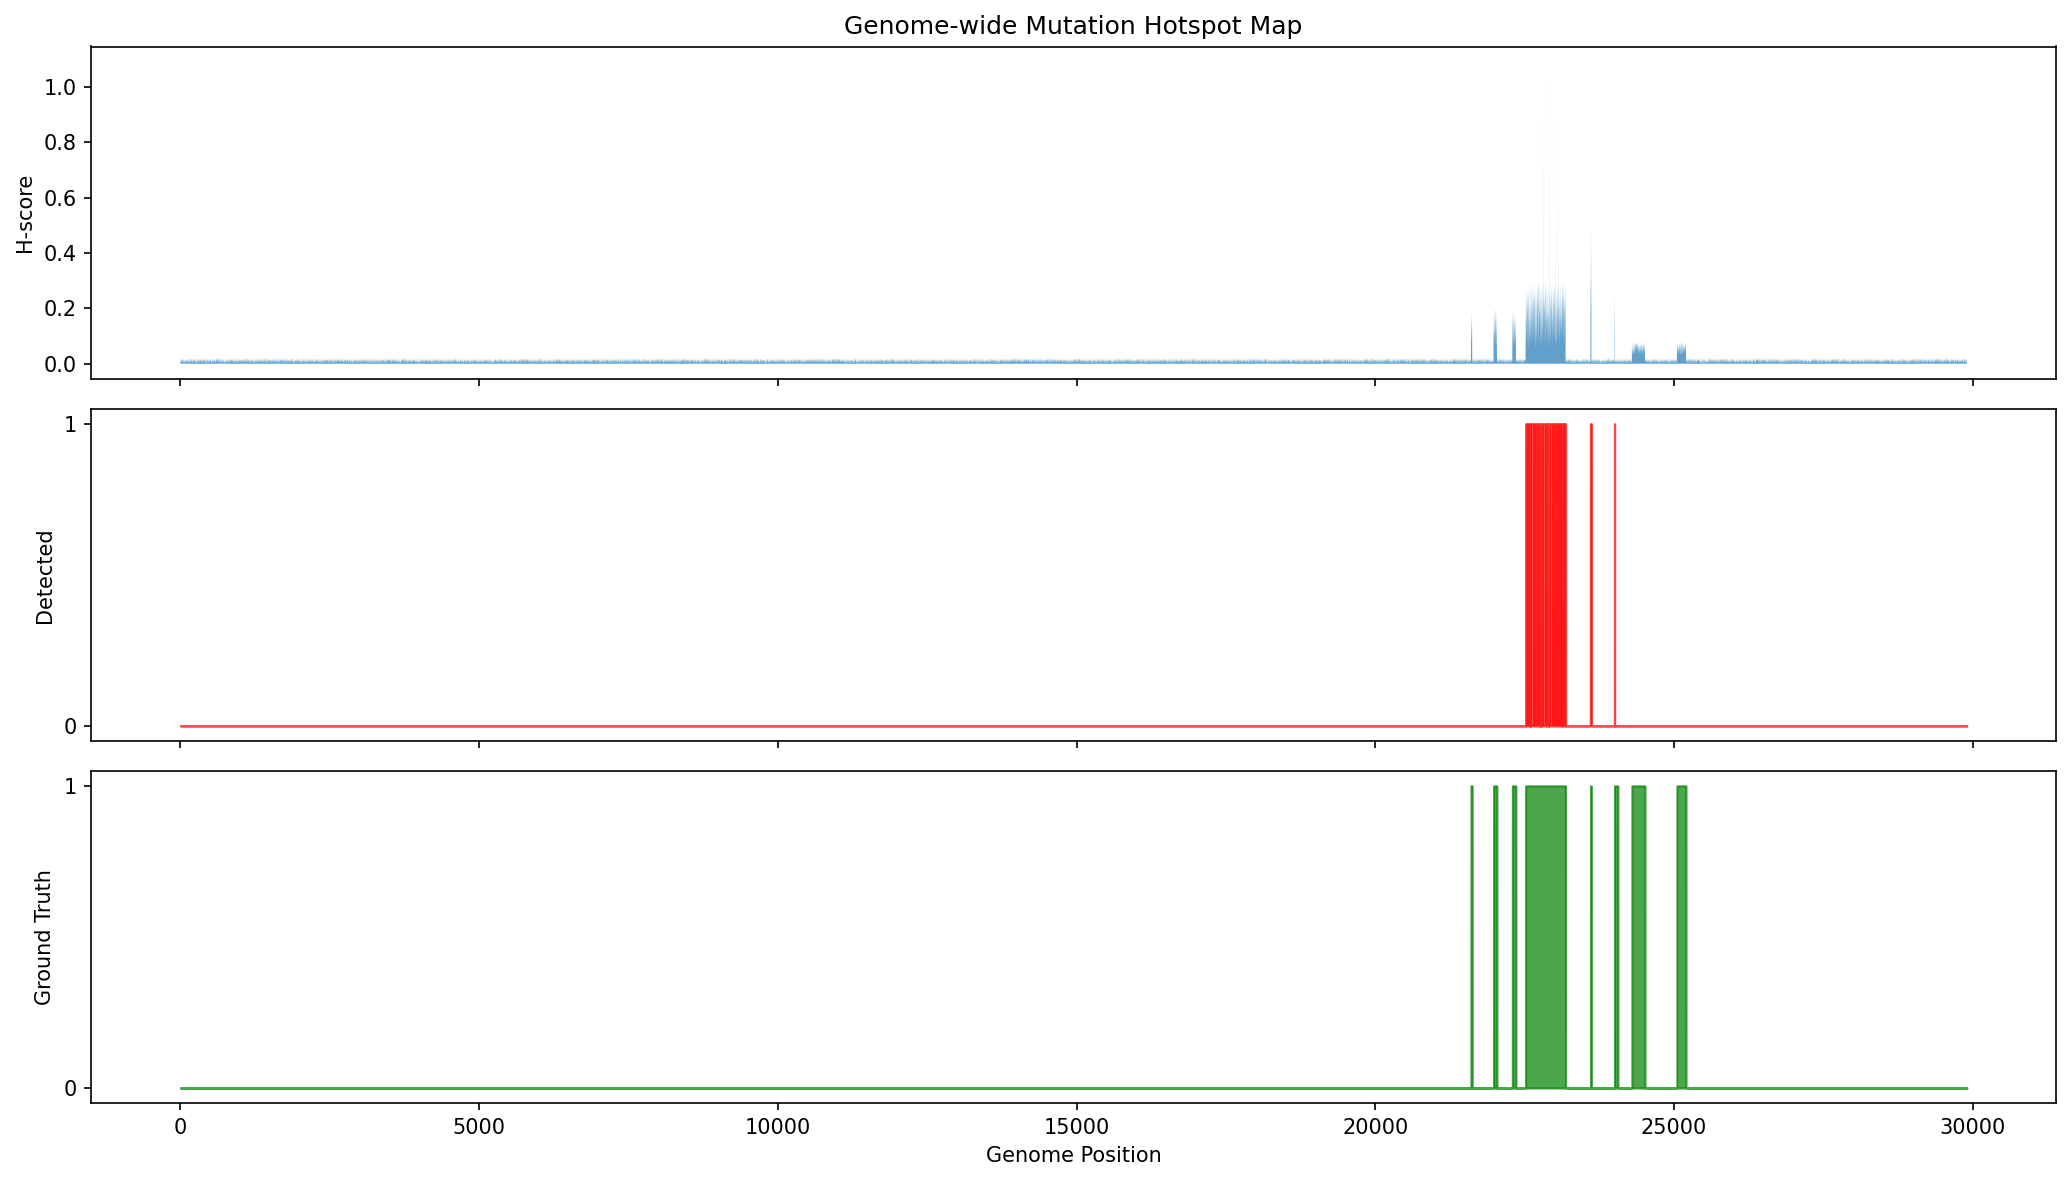
\includegraphics[width=\textwidth]{genome_hotspot_map.png}
\caption{SARS-CoV-2 Spike 단백질의 게놈 전체 핫스팟 맵. Ground truth로 사용된 7개의 주석된 기능 영역(RBD, NTD 항원 초과부위, 퓨린 절단 부위, S2' 절단 부위, 융합 펩타이드, HR1, HR2)이 뉴클레오티드 좌표에 매핑되어 있으며, 1,251개의 고유 Spike 뉴클레오티드 위치를 포함한다.}
\label{fig:mutbench_hotspot_map}
\end{figure}

\subsubsection{구성요소 2: 탐지 방법}

5가지 MutClust 변이체와 2가지 기준선 방법을 비교 평가한다.
각 변이체의 특성은 표~\ref{tab:variants}에 요약하였다.

\begin{table}[htbp]
\centering
\caption{MutBench에서 평가된 탐지 방법}
\label{tab:variants}
\footnotesize
\adjustbox{max width=\textwidth}{
\begin{tabular}{lp{2.5cm}p{8cm}}
\toprule
\textbf{방법} & \textbf{코드명} & \textbf{핵심 특성} \\
\midrule
MutClust-Original & v1-original & 원본 expand\_cluster (누적 감쇠 버그) \\
MutClust-Fixed & v2a-bugfix & 수정된 단일 단계 감쇠 공식 \\
MutClust-dNdS & v2b-bugfix+dnds & Fixed + dN/dS 양성 선택 필터 \\
MutClust-Hybrid & v2c-full & CCM 시드 + HDBSCAN 경계 + dN/dS \\
HDBSCAN-Auto & v3-hdbscan & 순수 HDBSCAN 자동 클러스터링 \\
\midrule
빈도 기준선 & --- & 상위 10백분위 H-score 역치 + 갭 기반 그룹화 \\
슬라이딩 윈도우 & --- & 20위치 이동 평균 + 10백분위 역치 \\
\bottomrule
\end{tabular}
}
\end{table}

\subsubsection{구성요소 3: 평가 지표}

위치 수준의 정밀도(precision), 재현율(recall), F1, 농축비(enrichment ratio), 부분추출 안정성(subsampling stability), 그리고 본 연구에서 새로 정의한 hotspot-score를 평가 지표로 사용한다.

\subsection{5가지 MutClust 변이체}
\label{subsec:variants}

\subsubsection{H-score 계산}
\label{subsec:mutbench_hscore}

MutClust는 각 게놈 위치에 대해 H-score를 계산한다:
\begin{equation}
H_i = \log_2(P_i \times E_i \times 100 + 1)
\label{eq:mutbench_hscore}
\end{equation}
여기서 $P_i$는 위치 $i$에서의 변이 비율의 합이고, $E_i$는 변이 유형의 Shannon 엔트로피이다.
Shannon 엔트로피는 다음과 같이 정의된다:
\begin{equation}
E_i = -\sum_{j=1}^{k} p_{ij} \log_2 p_{ij}
\label{eq:shannon_entropy}
\end{equation}
여기서 $p_{ij}$는 위치 $i$에서 변이 유형 $j$의 상대 빈도이고, $k$는 관찰된 변이 유형의 수이다.
H-score는 변이 빈도(해당 위치가 얼마나 자주 변이하는가)와 변이 다양성(얼마나 많은 치환 유형이 발생하는가)을 결합한다.

CCM(Core Candidate Mutation) 기준---H-score 역치 이상, 충분한 이웃 밀도, 최소 포인트 수---을 만족하는 위치가 시드로 선정된다.
expand\_cluster 함수는 의존성 기반 감쇠를 사용하여 각 시드를 양방향으로 확장한다:
\begin{equation}
D_\epsilon(t) = D_\epsilon^{\text{CCM}} - \frac{t}{d}
\label{eq:expand_cluster}
\end{equation}
여기서 $D_\epsilon^{\text{CCM}} = \lceil \gamma \times H_{\text{seed}} \rceil$은 시드의 초기 의존성 범위, $t$는 시드로부터의 거리, $d$는 감쇠 인자이다.

\subsubsection{버그 수정 (MutClust-Fixed)}
\label{subsec:improvements}

MutClust-Original의 expand\_cluster 함수에는 의존성 범위가 각 단계에서 누적적으로 차감되는 버그가 포함되어 있었으며, 이로 인해 가속되는 범위 축소가 발생하여 이론적 탐지 범위의 71--95\%가 손실되었다.
MutClust-Fixed는 시드의 의존성 범위로부터 직접 계산($D_\epsilon(t) = D_\epsilon^{\text{CCM}} - t/d$)하여 이를 수정하였으며, 합성 벤치마크에서 탐지 위치가 소폭 증가하고(641 vs. 637) 클러스터가 이론적 경계까지 확장되었다.

\subsubsection{dN/dS 선택 필터 (MutClust-dNdS)}

MutClust-dNdS는 비동의 대 동의 돌연변이 비율(dN/dS)을 기반으로 탐지 후 필터링을 추가한다.

\textbf{dN/dS 계산 방법.}
dN/dS 비율은 Nei--Gojobori 단순 계수 방법~\cite{nei1986simple}을 사용하여 클러스터별로 계산한다.
양성 선택(dN/dS $> 1.0$) 하의 클러스터만 유지하고, 중립 진화 또는 정화 선택 하의 클러스터는 제거한다.
짧은 클러스터(10개 미만 코돈)에서 dN/dS가 정의되지 않는 경우 해당 클러스터는 보수적으로 제외한다.

\textbf{뉴클레오티드 대 아미노산 수준.}
본 연구의 평가는 뉴클레오티드(nt) 수준에서 수행된다.
Spike 유전자(nt 21,563--25,384)는 3,822 뉴클레오티드(1,273 아미노산 + 종결 코돈)를 포함하며, H-score는 nt 위치별로 계산된다.
ground truth 기능 영역은 아미노산 수준에서 정의되므로(예: RBD = AA 319--541), 평가 시 각 AA 위치를 대응하는 3개 코돈 위치로 확장하여 nt 수준의 ground truth를 구성한다.
nt 수준 평가를 선택한 이유는 두 가지이다: (1) H-score가 코돈의 세 번째 위치(wobble position)에서도 변이 빈도를 독립적으로 포착하며, (2) 향후 비코딩 영역(5$'$/3$'$-UTR)으로의 확장을 고려하여 일관된 좌표 체계를 유지한다.

\textbf{삽입/결실(Indel) 처리.}
MutClust의 H-score 계산은 단일 뉴클레오티드 치환만을 대상으로 하며, 삽입 및 결실은 현재 처리되지 않는다.
이는 ins214EPE(Alpha/BA.1), $\Delta$69--70(Alpha), $\Delta$Y144(Alpha) 등 생물학적으로 중요한 indel이 H-score에 반영되지 않음을 의미한다.
향후 연구에서는 indel 빈도를 별도의 차원으로 통합하거나, indel 발생 위치에 가중치를 부여하는 확장이 필요하다.

정화 선택(dN/dS $< 1$) 또한 기능적으로 구속된 영역---예를 들어 융합 기구(HR1/HR2)와 필수 구조 도메인---을 나타내므로 생물학적으로 중요하다.
따라서 dN/dS $> 1.0$ 필터는 이러한 보존된 기능 영역의 재현율을 희생하는 대신, 면역 회피 및 수용체 적응과 같은 능동적 양성 선택 하의 부위 식별 정밀도를 향상시킨다.

\textbf{Jukes-Cantor 보정 검증.}
Jukes-Cantor 보정은 무시할 수 있는 변화만을 산출하여($\rho = 0.996$), 비보정 방법을 유지한다.

\subsubsection{HDBSCAN 하이브리드 (MutClust-Hybrid)}

MutClust-Hybrid는 MutClust의 도메인 특이적 CCM 시드 탐지와 HDBSCAN~\cite{campello2013hdbscan}의 자동 클러스터 경계 결정을 결합한다:

\begin{enumerate}
\item \textbf{시드 식별}: MutClust의 \texttt{is\_ccm()} 함수를 사용하여 변이 핫스팟 특성에 관한 도메인 지식을 보존한다.
\item \textbf{후보 수집}: 각 CCM 시드의 의존성 범위 내에서 비영(非零) H-score를 가진 모든 위치를 수집한다.
\item \textbf{HDBSCAN 클러스터링}: 후보 위치를 (i) $[0, H_{\max}]$ 범위로 min-max 정규화된 게놈 위치와 (ii) H-score 크기로 구성된 2차원 특성 공간에서 HDBSCAN으로 클러스터링한다. 이 정규화는 공간적 근접성과 점수 유사성에 동일한 가중치를 부여한다.
\item \textbf{dN/dS 필터링}: MutClust-dNdS와 동일한 양성 선택 신호 필터를 적용한다.
\end{enumerate}

이 하이브리드 접근법은 MutClust의 생물학적 사전 지식(CCM 기준)을 유지하면서 HDBSCAN의 데이터 기반 경계 탐지를 활용한다.

\textbf{계산 복잡도.}
MutClust-Hybrid의 전체 복잡도는 세 단계로 분해된다:
(1)~H-score 계산: $N$개 서열의 $M$개 위치에 대해 $O(NM)$;
(2)~CCM 시드 식별 및 후보 수집: H-score 정렬 $O(M \log M)$ 후 선형 스캔;
(3)~HDBSCAN 클러스터링: CCM 시드 주변의 $k$개 후보 위치에 대해 $O(k^2)$ (최소 신장 트리 구성).
실제로 $k \ll M$이며 (합성 벤치마크에서 $k \approx 800$, $M = 3{,}822$), 따라서 전체 복잡도는 $O(NM + M \log M)$에 지배되어 H-score 계산이 병목이다.
$N = 10{,}000$ 서열, $M = 3{,}822$ 위치에서 전체 파이프라인 실행 시간은 약 2초(단일 코어)로, 실시간 감시 환경에서도 실용적이다.

\subsubsection{순수 HDBSCAN (HDBSCAN-Auto)}

HDBSCAN-Auto는 MutClust를 완전히 우회하여, 적응형 역치(비영 H-score의 중앙값) 이상의 위치에 HDBSCAN을 직접 적용한다.
동일한 2차원 특성 공간(min-max 정규화 위치, H-score)을 사용하며, 수동으로 지정된 도메인 파라미터가 필요하지 않아 사전 조정 없이 모든 바이러스 게놈에 적용할 수 있다.
HDBSCAN-Auto는 min\_cluster\_size $= 5$, min\_samples $= 3$을 기본 파라미터로 사용한다.

\subsection{Hotspot-score 복합 지표}
\label{subsec:hotspot_score}

본 연구의 핵심 기여 중 하나인 hotspot-score는 세 가지 상보적 관점을 통합하는 복합 평가 지표이다:

\begin{equation}
\text{hotspot-score} = \frac{\text{recall} + \text{precision} + \text{stability}}{3}
\label{eq:hotspot_score}
\end{equation}

\begin{itemize}
\item \textbf{재현율(Recall)}: 탐지된 핫스팟 영역 내에 포착된 알려진 기능 위치의 비율. 생물학적 관련성을 평가한다---방법이 중요한 것을 찾아내는가?
\item \textbf{정밀도(Precision)}: ground truth와 중첩되는 탐지 위치의 비율. 특이도를 평가한다---방법이 위양성을 피하는가?
\item \textbf{안정성(Stability)}: 전체 데이터에 대한 탐지 결과와 100회 부분추출 실행 결과 간의 평균 Jaccard 유사도($J = |A \cap B| / |A \cup B|$). 각 반복에서 모든 게놈 위치에 대해 독립적으로 80\% 확률의 베르누이 마스크를 생성하고, 탈락한 위치(약 20\%)의 H-score를 0으로 설정한다(영점화). 게놈 좌표 체계는 유지되며, 영점화된 위치는 무신호 위치로 처리된다. 영점화된 H-score에 대해 동일한 탐지 방법을 재실행하고, 전체 데이터 탐지 결과와의 Jaccard 유사도를 산출한다. 재현성을 평가한다---데이터 교란 하에서 방법이 일관된 결과를 산출하는가?
\end{itemize}

세 구성 요소는 동일한 가중치를 받는다. 바이러스 감시 응용에서 높은 정확도이지만 데이터 교란에 불안정한 방법은 중간 정확도와 높은 재현성을 가진 방법보다 실용성이 낮으며, 안정성을 동일 구성 요소로 포함하는 것은 이 요구사항을 반영한다.

\noindent F1 점수 대신 재현율과 정밀도를 분리하여 안정성과 결합한 이유는, F1이 재현율·정밀도를 단일 값으로 축약함으로써 안정성과의 상호작용을 불투명하게 만들기 때문이다.
예를 들어, HDBSCAN-Auto의 F1(0.146)은 낮지만 재현율(0.944)과 안정성(0.788)은 높다.
F1 + 안정성 구조에서는 이 방법이 과소평가되지만, (재현율 + 정밀도 + 안정성)/3 구조에서는 높은 재현율과 안정성이 적절히 반영된다.

%% ============================================================
\section{점수화 및 탐지 방법}
\label{sec:scoring_detection_kr}

\subsection{스코어링 공식}
\label{subsec:9pathogen_scoring}

각 게놈 위치에 점수를 부여하는 9가지 스코어링 공식을 정의한다.
여기서 $P_i$는 위치 $i$의 변이 비율, $E_i$는 Shannon 엔트로피, $\text{rare}_i$는 희귀 변이 빈도(전체 변이 중 빈도 5\% 미만인 변이의 비율)이다.

\begin{enumerate}
\item \textbf{E*rare}: $S_i = E_i \times \text{rare}_i$. 엔트로피와 희귀 변이 빈도의 곱으로, 다양성이 높으면서 희귀 변이가 풍부한 위치를 강조한다.
\item \textbf{P*E*rare}: $S_i = P_i \times E_i \times \text{rare}_i$. 변이 빈도, 엔트로피, 희귀 변이를 모두 결합한다.
\item \textbf{minority\_E}: $S_i = f_{2\text{nd},i} \times E_i$. 두 번째로 빈번한 대립유전자 빈도($f_{2\text{nd}}$)와 엔트로피의 곱이다.
\item \textbf{P*minority\_E}: $S_i = P_i \times f_{2\text{nd},i} \times E_i$.
\item \textbf{P*E}: $S_i = P_i \times E_i$. 빈도와 엔트로피의 단순 곱이다.
\item \textbf{H-score}: $S_i = \log_2(P_i \times E_i \times 100 + 1)$. MutClust 원본 공식(식~\ref{eq:mutbench_hscore}).
\item \textbf{E\_only}: $S_i = E_i$. Shannon 엔트로피만 사용한다.
\item \textbf{P*E\textsuperscript{2}}: $S_i = P_i \times E_i^2$. 엔트로피에 이차 가중치를 부여한다.
\item \textbf{rank(P*E)}: $S_i = \text{rank}(P_i \times E_i) / N$. P*E의 순위를 정규화한 비모수적 점수이다.
\end{enumerate}

\subsection{다중 Ground Truth를 위한 대안적 스코어링 방법}
\label{subsec:alternative_scoring}

시간적 검증(제~\ref{sec:temporal}절)에서 H-score 포화가 확인됨에 따라, 다양한 ground truth 정의에 대한 상보적 평가를 수행하기 위해 다음의 대안적 스코어링 방법을 설계하였다.
이 방법들은 핫스팟 ``탐지'' 방법이 아니라 각 게놈 위치에 점수를 부여하는 ``스코어링'' 접근법으로, 역치 기반으로 상위 위치를 선별하여 다중 ground truth와 비교한다.

\textbf{Original H-score}: MutClust의 원래 H-score 공식(식~\ref{eq:mutbench_hscore})을 그대로 사용한다.

\textbf{Saturated H-score}: 2024--2025 데이터에서 동시대 합의서열 정렬을 통해 계산된 H-score로, 참조 서열(Wuhan-Hu-1) 대비가 아닌 현재 집단 내 변이를 반영한다.

\textbf{CH-score (Consensus-based H-score)}: 현재 합의서열 대비 변이 빈도를 계산하여, 참조 서열 의존성을 제거한 H-score 변형이다:
\begin{equation}
\text{CH}_i = \log_2(P_i^{\text{consensus}} \times E_i \times 100 + 1)
\end{equation}
여기서 $P_i^{\text{consensus}}$는 합의서열 대비 비합의 아미노산 빈도이다.

\textbf{E-score (Entropy-only score)}: Shannon 엔트로피만을 사용하여, 빈도 항($P_i$)을 제거하고 위치별 다양성만으로 점수를 부여한다:
\begin{equation}
\text{E-score}_i = -\sum_{a} f_{a,i} \log_2 f_{a,i}
\end{equation}

\textbf{TC-freq (Temporal Contrast frequency)}: 두 시간대 간 변이 빈도의 변화율을 측정한다:
\begin{equation}
\text{TC-freq}_i = \frac{|\text{freq}_{t_2}(i) - \text{freq}_{t_1}(i)|}{\text{freq}_{t_1}(i) + \epsilon}
\end{equation}
여기서 $\text{freq}_{t}(i)$는 시간대 $t$에서 위치 $i$의 비참조 아미노산 빈도이며, $\epsilon = 10^{-6}$은 영 나눗셈 방지 상수이다.

\textbf{TC-freq-v2}: TC-freq에 절대 빈도 가중치를 추가한 변형으로, $\text{TC-freq-v2}_i = \text{TC-freq}_i \times \text{freq}_{t_2}(i)$이다.

\textbf{TC-freq-v3}: 분기별(quarterly) 시간 윈도우를 사용하는 변형으로, 연간 전체 비교 대신 각 분기 간 빈도 변화의 최대값을 취한다.

\textbf{dN/dS-weighted CH}: CH-score에 위치별 dN/dS 비율을 가중치로 적용한 변형이다.

각 스코어링 방법에 대해 상위 5\%, 10\%, 20\% 및 중위수 기반 역치를 적용하여 ``탐지된'' 위치 집합을 생성하고, 각 ground truth에 대한 F1, 농축비(enrichment ratio), Cohen's $d$ 효과 크기를 산출한다.

\subsection{탐지 방법 패밀리}
\label{subsec:9pathogen_detection}

15개 알고리즘 패밀리에 속하는 총 41개 탐지 방법을 평가한다.
각 탐지 방법은 스코어링 공식이 부여한 위치별 점수 프로파일로부터 핫스팟 영역을 식별한다.

\begin{table}[htbp]
\centering
\caption{9-병원체 벤치마크에서 평가된 41개 탐지 방법 (15개 패밀리)}
\label{tab:detection_families}
\small
\adjustbox{max width=\textwidth}{
\begin{tabular}{llr}
\toprule
\textbf{패밀리} & \textbf{방법 설명} & \textbf{변이체 수} \\
\midrule
Wavelet & 웨이블릿 변환 기반 다중해상도 피크 탐지 & 3 \\
KDE & 커널 밀도 추정 기반 핫스팟 탐지 & 3 \\
SlidingTest & 슬라이딩 윈도우 통계 검정 & 2 \\
GradPeak & 점수 프로파일의 기울기 피크 탐지 & 2 \\
LocalContrast & 국소 대비(local--global 비율) 기반 탐지 & 3 \\
CUSUM & 누적합 변화점 탐지 & 3 \\
AdaptiveKnee & 적응형 곡률 기반 역치 & 1 \\
ScoreDBSCAN & 점수 기반 밀도 공간 클러스터링 & 2 \\
Spectral & 스펙트럼 분석 기반 주기적 패턴 탐지 & 2 \\
Bayes & 베이지안 변화점 탐지 & 2 \\
\midrule
Ensemble & 다수결 앙상블 & 2 \\
AdaptWin & 적응형 윈도우 크기 탐지 & 2 \\
FreqThresh & 빈도 백분위 역치 (top-$k$\%) & 4 \\
SWAN & 슬라이딩 윈도우 적응형 정규화 & 9 \\
MutClust-Orig & MutClust 원본 알고리즘 & 1 \\
\midrule
\textbf{합계} & & \textbf{41} \\
\bottomrule
\end{tabular}
}
\end{table}

41개 방법은 15개 알고리즘 패밀리로부터, 각각 서로 다른 파라미터 설정으로 인스턴스화하여 도출된다(표~\ref{tab:detection_variants}).
예를 들어, Wavelet 패밀리는 3가지 피크 탐지 역치($t = 1.0, 1.5, 2.0$ 표준편차)로 검정하고, FreqThresh는 4가지 백분위 절단값(상위 1\%, 3\%, 5\%, 10\%)으로 검정한다.
이 다중 파라미터 설계는 벤치마크가 각 알고리즘 패밀리를 단일의 잠재적으로 차선인 작동점이 아닌, 다양한 민감도--특이도 절충 범위에 걸쳐 평가하도록 보장한다.

\begin{table}[htbp]
\centering
\caption{탐지 방법 패밀리별 파라미터 변이체 (총 41개 방법)}
\label{tab:detection_variants}
\small
\adjustbox{max width=\textwidth}{
\begin{tabular}{llrl}
\toprule
\textbf{패밀리} & \textbf{파라미터} & \textbf{변이체 수} & \textbf{값} \\
\midrule
Wavelet & CWT 피크 역치 $t$ & 3 & $t = 1.0, 1.5, 2.0$ (std. dev.) \\
KDE & 대역폭 배수 & 3 & $0.5\times, 1.0\times, 2.0\times$ Silverman \\
SlidingTest & 윈도우 크기 & 2 & 20, 50 positions \\
GradPeak & 평활화 윈도우 & 2 & 5, 11 positions \\
LocalContrast & 국소 윈도우 크기 & 3 & 10, 20, 50 positions \\
CUSUM & 드리프트 파라미터 $\delta$ & 3 & $\delta = 0.5, 1.0, 2.0$ \\
AdaptiveKnee & (파라미터 없음) & 1 & 자동 knee point 탐지 \\
ScoreDBSCAN & Epsilon & 2 & $\varepsilon = 10, 15$ \\
Spectral & 고역 통과 절단값 & 2 & 상위 5\%, 10\% 주파수 \\
Bayes & 사전 확률 & 2 & $\pi = 0.05, 0.10$ \\
Ensemble & 하위 탐지기 집합 & 2 & 3-of-4, 4-of-4 다수결 \\
AdaptWin & 확장 역치 & 2 & 50th, 75th 백분위 \\
FreqThresh & 상위 $k$\% 절단값 & 4 & $k = 1, 3, 5, 10$ \\
SWAN & 윈도우 $\times$ 정규화 & 9 & $w \in \{20,50,100\} \times \{z, \text{min-max}, \text{robust}\}$ \\
MutClust-Orig & (고정) & 1 & 원본 CCM + 적응형 DBSCAN \\
\midrule
\textbf{합계} & & \textbf{41} & \\
\bottomrule
\end{tabular}
}
\end{table}

표~\ref{tab:detection_prior_apps}는 각 탐지 방법 패밀리의 바이러스학 및 유전체학 연구에서의 선행 적용 사례를 요약하여, 바이러스 변이 핫스팟 탐지로의 적용 맥락을 제공한다.

\begin{table}[htbp]
\centering
\caption{탐지 방법 패밀리의 바이러스학 및 유전체학 연구 선행 적용}
\label{tab:detection_prior_apps}
\small
\adjustbox{max width=\textwidth}{
\begin{tabular}{llp{5.5cm}l}
\toprule
\textbf{패밀리} & \textbf{접근 유형} & \textbf{선행 적용} & \textbf{참고문헌} \\
\midrule
Wavelet & 신호 처리 & 유전체 서열 주기성 탐지 & \cite{anastassiou2001genomic} \\
KDE & 밀도 추정 & 커널 평활화를 통한 ChIP-Seq 피크 호출 & \cite{zhang2008chipseq} \\
SlidingTest & 슬라이딩 윈도우 검정 & 슬라이딩 윈도우 중립성 검정 (Tajima's D) & \cite{tajima1989statistical} \\
GradPeak & 피크 탐지 & 점수 프로파일에서의 ChIP-Seq 피크 탐지 & \cite{zhang2008chipseq} \\
LocalContrast & 국소 z-점수 & 복제수 변이 분할 & \cite{olshen2004cnv} \\
CUSUM & 변화점 탐지 & 생물감시 발병 탐지 & \cite{sonesson2003cusum} \\
AdaptiveKnee & Knee point 탐지 & 최적 클러스터 수 선택 (Kneedle) & \cite{satopaa2011kneedle} \\
ScoreDBSCAN & 밀도 클러스터링 & 암 돌연변이 핫스팟 탐지 & \cite{tokheim2016hotmaps} \\
Spectral & 푸리에 분석 & 유전체 신호 처리 & \cite{anastassiou2001genomic} \\
Bayes & 베이지안 탐지 & 암 드라이버 돌연변이 탐지 (MutSigCV) & \cite{lawrence2013mutsigcv} \\
\midrule
Ensemble & 다수결 투표 & 암 드라이버 유전자 식별 & \cite{bailey2018comprehensive} \\
AdaptWin & 적응형 윈도우 & 유전체 복제수 분할 & \cite{picard2011genomicseg} \\
FreqThresh & 빈도 역치 & SARS-CoV-2 지리적 변이 빈도 & \cite{mercatelli2020geographic} \\
SWAN & 슬라이딩 윈도우 정규화 & 본 연구에서 최초 제안 & --- \\
MutClust-Orig & 밀도 기반 클러스터링 & SARS-CoV-2 변이 핫스팟 탐지 & \cite{youn2025mutclust} \\
\bottomrule
\end{tabular}
}
\end{table}

\noindent 15개 패밀리는 아래 5개 범주로 분류된다.

\textbf{역치 기반} (FreqThresh, AdaptiveKnee, AdaptWin).
점수 절단값을 적용하여 핫스팟을 선정한다: FreqThresh는 고정 백분위 역치(상위 $k$\%)를 사용하고, AdaptiveKnee는 정렬된 점수 곡선에서 knee point를 자동 탐지하며, AdaptWin은 백분위 역치 이상의 시드 위치를 양방향으로 확장한다.

\textbf{신호 처리} (Wavelet, Spectral, CUSUM).
점수 프로파일을 변환하여 이상 영역을 식별하는 방법이다: Wavelet은 Mexican hat 커널로 다중 스케일 연속 웨이블릿 변환을, Spectral은 FFT 기반 고역 통과 필터링으로 국소 편차 분리를, CUSUM은 $z$-정규화 프로파일에 누적합 제어 차트를 적용한다.

\textbf{밀도 및 클러스터링} (KDE, ScoreDBSCAN).
KDE는 점수 가중 위치 프로파일에 Gaussian 커널 밀도 추정을 적용하여 백분위로 역치화한다. ScoreDBSCAN은 위치를 (좌표, 점수) 2차원 공간에 매핑하고 축 재조정 후 DBSCAN 클러스터링을 적용한다.

\textbf{통계 및 모델 기반} (SlidingTest, LocalContrast, GradPeak, Bayes, SWAN).
배경으로부터 유의하게 이탈하는 위치 또는 윈도우를 식별하는 통계적 방법이다: SlidingTest와 SWAN은 슬라이딩 윈도우 $z$-검정을, LocalContrast는 국소 $z$-점수를, GradPeak는 평활화 프로파일에서 현저도 필터링 피크 탐지를, Bayes는 사전확률과 정규화 점수로부터 사후 핫스팟 확률을 산출한다.

\textbf{앙상블 및 레거시} (Ensemble, MutClust-Orig).
Ensemble은 4개의 간이 하위 탐지기를 다수결 투표로 결합한다. MutClust-Orig는 원본 MutClust 로직(CCM 시드 + 적응형 DBSCAN)을 MSA 기반 점수 프로파일에 적용한다.

%% ============================================================
\section{평가 및 통계 설계}
\label{sec:eval_stat_design_kr}

\subsection{평가 지표}
\label{subsec:9pathogen_metrics}

9-병원체 벤치마크에서는 다음의 평가 지표를 사용한다.

\begin{itemize}
\item \textbf{MCC (Matthews Correlation Coefficient)}: 주요 평가 지표(식~\ref{eq:mcc}에 공식 정의).
혼동행렬은 Layer A(양성 선택 위치)만을 양성 레이블로 사용하여 구성된다: TP = 탐지되었으며 Layer A에 속하는 위치, FP = 탐지되었으나 Layer A에 속하지 않는 위치, FN = 탐지되지 않았으나 Layer A에 속하는 위치, TN = 탐지되지 않았으며 Layer A에도 속하지 않는 위치.
Layer B(구속 영역)는 MCC 계산에 포함되지 않으며 별도의 constrained FPR로 평가된다. Layer A에도 B에도 속하지 않는 다수의 게놈 위치는 탐지 여부에 따라 FP 또는 TN으로 분류된다.
\item \textbf{F1}: 정밀도와 재현율의 조화 평균.
\item \textbf{정밀도(Precision)}: 탐지된 위치 중 실제 양성의 비율.
\item \textbf{재현율(Recall)}: 실제 양성 중 탐지된 비율.
\item \textbf{농축비(Enrichment ratio)}: 탐지 영역 내 양성 밀도 대비 전체 양성 밀도의 비율.
\item \textbf{구속 영역 FPR (Constrained FPR)}: Layer B 구속 영역에서의 위양성률.
\item \textbf{DMS F1}: Layer C DMS ground truth에 대한 F1 점수 (4종 병원체에서만 산출).
\end{itemize}

Stage~1에서는 안정성을 포함하는 hotspot-score를 사용하여 단일 병원체 심층 분석을 수행하지만, Stage~2에서는 안정성의 교차 병원체 비교 가능성이 검증되지 않았고 MCC가 극단적 클래스 불균형에 더 적합하므로 MCC를 주 평가 지표로 채택한다.
이 설계 결정은 세 가지 고려에 의해 동기 부여된다.
첫째, 안정성 구성 요소는 위치 수준 부분추출 하의 부트스트랩 재현성을 측정하나, 정렬 길이(340--1,330 AA)와 MSA 크기(530--5,019 고유 서열)가 상이한 병원체 간에 부분추출 행동이 근본적으로 다르므로, 교차 병원체 안정성 값의 비교 가능성이 보장되지 않는다.
둘째, MCC는 혼동행렬의 네 셀(TP, TN, FP, FN) 모두를 활용하여, 핫스팟 탐지에 내재하는 극단적 클래스 불균형(9종 병원체의 양성률 1--16\%) 하에서 균형 잡힌 평가를 제공한다.
셋째, 단계 간 평가 지표를 분리함으로써 1단계에서는 탐지의 \textit{신뢰성}(안정성)을, 2단계에서는 탐지의 \textit{정확성}(MCC)을 각 분석 목적에 맞게 평가할 수 있다.
MCC는 다음과 같이 정의된다:
\begin{equation}
\text{MCC} = \frac{TP \times TN - FP \times FN}{\sqrt{(TP+FP)(TP+FN)(TN+FP)(TN+FN)}}
\label{eq:mcc}
\end{equation}
여기서 $TP$, $TN$, $FP$, $FN$은 각각 진양성, 진음성, 위양성, 위음성이다.
MCC는 $-1$(완전 불일치)에서 $0$(무작위 예측)을 거쳐 $+1$(완전 예측)의 범위이며, F1과 달리 혼동행렬의 네 셀 모두를 활용하므로 클래스 불균형에 강건하다.
분모의 어떤 인수가 0일 때(예: 양성 예측 없음), MCC는 관례적으로 0으로 정의한다.
MCC를 주요 지표로 선택한 이유는, 핫스팟 탐지에서 양성 위치(수렴 진화 부위)가 전체 게놈의 소수를 차지하는 불균형 분류 문제에서 F1보다 균형 잡힌 평가를 제공하기 때문이다. Chicco and Jurman~\cite{chicco2020mcc}은 불균형 이진 분류에서 MCC가 F1 및 정확도보다 유의미한 평가를 제공함을 체계적으로 입증하였다.
1단계에서 사용된 안정성 구성 요소는 외부 ground truth와 독립적인 내부 일관성 지표이며, 9종 병원체 간 서열 길이 및 MSA 크기의 차이에 따른 Bernoulli 마스킹 효과의 병원체 간 비교 가능성이 검증되지 않아 2단계에서는 제외하였다.

\subsection{통계 분석 설계}
\label{subsec:9pathogen_statistics}

\subsubsection{Three-way ANOVA ($\omega^2$)}

스코어링 공식(9수준), 탐지 패밀리(15수준), 병원체(9수준)의 세 요인에 대한 삼원분산분석(three-way ANOVA)을 수행한다.
효과 크기로 편향 보정된 $\omega^2$ (omega-squared)를 사용하며, 이는 $\eta^2$가 표본 크기에 따라 상향 편향되는 문제를 회피한다. $\omega^2$ 값은 Cohen의 효과 크기 기준~\cite{cohen1988statistical}에 따라 0.01(소), 0.06(중), 0.14 이상(대)으로 해석된다:
\begin{equation}
\omega^2 = \frac{SS_{\text{effect}} - df_{\text{effect}} \times MS_{\text{error}}}{SS_{\text{total}} + MS_{\text{error}}}
\label{eq:omega_squared}
\end{equation}
주효과(main effect)와 이원 상호작용(two-way interaction)의 $\omega^2$를 비교하여, 성능 변동의 주요 원천을 식별한다.

\subsubsection{LOPO 교차 검증 (Leave-One-Pathogen-Out)}

9종 병원체 중 1종을 제외한 8종에서 최적 조합(스코어링 $\times$ 탐지)을 선정하고, 제외된 병원체에 적용하여 일반화 성능을 평가한다.
9회 반복하여 훈련 최적 조합과 테스트 최적 조합(oracle)의 일치율 및 성능 격차를 산출한다.

\subsubsection{Friedman 검정}

9개 병원체를 블록으로 사용하는 비모수적 반복측정 검정으로, 상위 $k$개 조합 간에 통계적으로 유의한 성능 차이가 존재하는지를 검정한다.

\subsubsection{병원체 수준 BCa 부트스트랩 신뢰 구간}

9개 병원체의 MCC 값에 대해 편향 보정 가속(BCa, bias-corrected and accelerated) 부트스트랩 신뢰 구간을 산출하여, 최적 조합의 병원체 간 성능 변동성을 정량화한다.

\subsubsection{하위표본 강건성 분석}

MSA 서열의 25\%, 50\%, 75\%, 100\% 비율로 무작위 하위표본을 추출하여 벤치마크를 반복 수행하고, 표본 크기에 따른 MCC 안정성을 검증한다.

\textbf{Hotspot-score 가중치 민감도 분석.}
\label{subsec:weight_sensitivity_methods}
Hotspot-score의 세 구성 요소에 동일 가중치($1/3$)를 부여하는 것의 강건성을 검증하기 위해, 일반화된 가중 hotspot-score를 정의한다:
\begin{equation}
\text{hotspot-score}_w = w_r \cdot \text{recall} + w_p \cdot \text{precision} + w_s \cdot \text{stability}
\label{eq:weighted_hotspot_score}
\end{equation}
여기서 $w_r + w_p + w_s = 1$이며 각 가중치는 $[0.05, 0.95]$ 범위이다.
총 171개의 가중치 조합에 대해 5가지 방법의 순위를 계산하여, MutClust-Hybrid가 1위를 유지하는 가중치 공간의 비율(순위 강건성, rank robustness)을 분석한다.
또한 조기경보(recall 중시), 백신 설계(precision 중시), 모니터링(stability 중시) 등 7개 응용 시나리오에 대한 순위를 별도로 제시한다.

\textbf{통계적 검증 방법.}
\label{subsec:statistical_methods}
벤치마크 결과의 통계적 견고성을 평가하기 위해 다음 세 가지 방법을 적용한다.

\textbf{부트스트랩 신뢰 구간}: 7개 기능 영역을 단위로 한 영역 수준 부트스트랩(region-level bootstrap)을 수행한다.
각 반복에서 7개 영역을 복원추출하여 부트스트랩 ground truth를 구성하고, 전체 데이터에서의 탐지 결과를 이 부트스트랩 ground truth에 대해 재평가한다.
이 설계는 ground truth 정의의 불확실성---어떤 기능 영역을 포함하느냐에 따른 평가 변동---을 포착하며, 개별 위치 리샘플링에서 발생하는 유효 크기 축소 편향을 회피한다.

\textbf{순열 검정(Permutation test)}: 두 가지 순열 접근법을 사용한다.
(1)~\textit{무작위 레이블 섞기}: 1,000회의 ground truth 레이블 무작위 순열을 통해 관찰된 지표가 무작위 기대를 유의하게 초과하는지 검정한다.
(2)~\textit{순환 순열(Circular permutation)}: H-score 벡터를 무작위 오프셋 $k$만큼 회전시켜($H_i \rightarrow H_{(i+k) \bmod N}$), 회전된 점수에서 핫스팟을 재탐지하고 원래 ground truth에 대해 평가한다.
이 접근법은 H-score의 공간적 자기상관 구조(클러스터 패턴)를 보존하면서 게놈 위치와의 관계만 무작위화하여, 무작위 레이블 섞기보다 보수적인 귀무 분포를 생성한다.
p-값은 $count / n_{\text{perm}}$ (귀무 분포에서 관측값 이상인 비율)으로 산출한다.

\textbf{쌍별 비교}: 동일 부트스트랩 리샘플에서 두 방법을 동시에 평가하는 paired bootstrap 설계로, 방법 간 hotspot-score 차이의 통계적 유의성을 검정한다.


% Chapter 4: 실험 결과
\chapter{실험 결과}
\label{ch:results}

본 장에서는 제~\ref{ch:mutbench}장에서 제시한 MutBench 프레임워크의 실험 결과를 2단계 구조로 보고한다.

\textbf{1단계 (깊이 우선, 제~\ref{sec:variant_comparison}--\ref{sec:phylo_simulation}절):}
SARS-CoV-2 단일 병원체에서 5가지 MutClust 변이체와 2가지 기준선 방법의 성능을 정밀 비교한다.
합성 벤치마크, DMS 검증, 민감도 분석, 시간적 일반화, 다중 ground truth 평가, 교차 병원체 예비 검증(H3N2)을 통해, ``탐지 전략의 선택이 파라미터 조정보다 성능에 결정적이며, 최적 방법이 데이터 분포 특성에 의존한다''는 교훈을 도출한다.

\textbf{2단계 (너비 우선, 제~\ref{sec:9pathogen_results}절):}
1단계의 교훈을 일반화하기 위해, 9종 병원체 $\times$ 9가지 스코어링 $\times$ 41개 탐지 방법으로 확장한 대규모 벤치마크를 수행한다.
1단계의 MutClust 변이체들은 단일 알고리즘의 구조적 변형이므로, 2단계에서는 원본(MutClust-Original)만을 대표로 포함하고 다양한 알고리즘 패밀리(Wavelet, KDE, CUSUM, Bayesian 등)의 독립 방법과 비교한다.

%% ============================================================
\section{합성 벤치마크: 변이체 비교}
\label{sec:variant_comparison}

합성 H-score를 사용하여 SARS-CoV-2 유사 게놈(29,903 위치)에서 7개 기능 영역(1,251개 고유 ground truth 뉴클레오티드 위치)을 대상으로 방법을 비교하였다.
제~\ref{ch:mutbench}장에서 기술한 바와 같이, 이 합성 벤치마크는 통제된 신호 복원 검정으로서 알려진 위치에 삽입된 신호의 복원 능력을 평가한다.
결과는 표~\ref{tab:method_comparison}에 제시하였다.

\begin{table}[htbp]
\centering
\caption{합성 SARS-CoV-2 데이터에 대한 방법 비교 (29,903 위치, 1,251개 ground truth 기능 뉴클레오티드 위치)}
\label{tab:method_comparison}
\begin{tabular}{lrrrrrr}
\toprule
\textbf{방법} & \textbf{정밀도} & \textbf{재현율} & \textbf{F1} & \textbf{농축비} & \textbf{탐지 수} & \textbf{클러스터} \\
\midrule
MutClust-Original & 0.991 & 0.504 & 0.668 & 23.68 & 637 & 31 \\
MutClust-Fixed & 0.988 & 0.506 & 0.669 & 23.60 & 641 & 30 \\
MutClust-dNdS$^\dagger$ & 0.988 & 0.506 & 0.669 & 23.60 & 641 & 30 \\
MutClust-Hybrid & 0.968 & 0.659 & 0.785 & 23.15 & 852 & 8 \\
HDBSCAN-Auto & 0.079 & 0.944 & 0.146 & 1.89 & 14,916 & 21 \\
\midrule
빈도 기준선 & 0.404 & 0.965 & 0.569 & 9.65 & 2,991 & 1,587 \\
슬라이딩 윈도우 & 0.157 & 0.974 & 0.270 & 3.75 & 7,773 & 214 \\
\bottomrule
\end{tabular}
\begin{minipage}{\textwidth}
\smallskip
\footnotesize $^\dagger$합성 데이터에서는 dN/dS 계산을 위한 참조 서열이 제공되지 않으므로, MutClust-Fixed와 동일한 결과를 산출한다.
\end{minipage}
\end{table}

결과는 탐지 전략 간의 명확한 정밀도--재현율 절충을 드러낸다.
CCM 기반 시드 탐지를 사용하는 MutClust 변이체(Original, Fixed, dNdS)는 거의 완벽한 정밀도($> 0.98$)를 달성하지만 중간 수준의 재현율(0.50--0.51)을 보이며, 이는 CCM 탐지가 주로 고신호 핫스팟 영역(RBD, 퓨린 절단)을 식별하면서 저신호 기능 부위(NTD 초과부위, HR1/HR2)를 놓치는 것을 반영한다.
버그 수정은 정밀도를 유지하면서 탐지 위치를 4개 확장하였다(641 vs. 637).

MutClust-Hybrid는 CCM 시드 탐지와 HDBSCAN 경계 결정을 결합하여 최고 F1(0.785)을 달성하였다.
정밀도(0.968)는 CCM 전용 변이체에 근접하면서 재현율(0.659)이 크게 향상되었으며, HDBSCAN의 더 넓은 경계 추정을 통해 NTD 초과부위의 일부를 포함한 추가 기능 영역을 포착하였다.

HDBSCAN-Auto는 최고 재현율(0.944)을 달성하였으나 낮은 정밀도(0.079)를 보이며, 14,916개 위치---게놈의 약 절반---를 21개 클러스터에서 탐지하였다.
CCM 시드 탐지가 후보 공간을 제한하지 않으면 HDBSCAN이 실제 기능 부위와 함께 상당한 배경 잡음을 포착함을 보여준다.
이는 도메인 특이적 사전 지식이 탐지 특이성을 실질적으로 향상시킴을 입증한다.

\textbf{외부 기준선 비교.}
빈도 기준선(H-score 역치 초과 위치 탐지)과 슬라이딩 윈도우(고정 크기 창의 평균 H-score 역치)는 모두 높은 재현율(0.965, 0.974)을 달성하지만 낮은 정밀도(0.404, 0.157)를 보인다.
이 기준선들의 F1(0.569, 0.270)은 모든 MutClust 변이체(0.668--0.785)보다 낮으며, 특히 MutClust-Hybrid 대비 F1 격차가 0.216--0.515에 달한다.
빈도 기준선은 적응적 클러스터 크기 결정 능력이 없어 2,991개 위치를 1,587개의 독립 ``클러스터''로 탐지하며, 슬라이딩 윈도우는 고정 창 크기의 제약으로 7,773개 위치를 과잉 탐지한다.
이 결과는 MutClust의 CCM 기반 적응형 밀도 추정이 단순 역치·윈도우 기반 접근법 대비 실질적인 성능 향상을 제공함을 확인한다.

Hotspot-score를 포함한 확장된 평가 지표는 표~\ref{tab:hotspot_scores}에 제시하였다.

\begin{table}[htbp]
\centering
\caption{Hotspot-score 분석 (100회 부분추출, 80\% 위치 유지)}
\label{tab:hotspot_scores}
\begin{tabular}{lrrrr}
\toprule
\textbf{방법} & \textbf{정밀도} & \textbf{재현율} & \textbf{안정성} & \textbf{Hotspot-score} \\
\midrule
MutClust-Original & 0.991 & 0.504 & 0.418 & 0.638 \\
MutClust-Fixed & 0.988 & 0.506 & 0.445 & 0.646 \\
MutClust-dNdS & 0.988 & 0.506 & 0.445 & 0.646 \\
\textbf{MutClust-Hybrid} & \textbf{0.968} & \textbf{0.659} & \textbf{0.706} & \textbf{0.778} \\
HDBSCAN-Auto & 0.079 & 0.944 & 0.788 & 0.604 \\
\bottomrule
\end{tabular}
\end{table}

Hotspot-score는 F1만으로는 포착할 수 없는 평가 차원을 드러내며, \textbf{MutClust-Hybrid를 최우수 방법}(hotspot-score 0.778)으로 식별한다.
MutClust-Hybrid의 우위는 세 차원 모두에서의 강한 성능에서 비롯된다: 거의 완벽한 정밀도(0.968), 향상된 재현율(0.659), 높은 안정성(0.706).
CCM 시드 탐지를 유지하면서 HDBSCAN을 경계 결정에 사용함으로써, 순수 CCM 탐지가 놓치는 기능 영역(예: 저신호 NTD 초과부위 위치)을 포착하면서 도메인 특이적 사전 지식의 특이성 이점을 보존한다.

HDBSCAN-Auto는 최고 개별 안정성(0.788)과 재현율(0.944)을 달성하지만, 낮은 정밀도(0.079)로 인해 MutClust 변이체 중 최저 hotspot-score(0.604)를 기록한다.
이는 복합 지표의 가치를 잘 보여준다: 재현율만으로 HDBSCAN-Auto를 평가하면 최우수 방법으로 순위가 매겨지고, 정밀도만으로 평가하면 완전히 기각될 것이다.
Hotspot-score는 하이브리드 접근법을 최적 균형으로 올바르게 식별하는 균형 잡힌 평가를 제공한다(그림~\ref{fig:mutbench_method_comparison}).

\textbf{2단계 파이프라인 검증.}
HDBSCAN-Auto의 높은 재현율과 MutClust-Hybrid의 높은 정밀도를 결합하기 위해, 2단계 탐지 파이프라인을 추가적으로 검증하였다.
HDBSCAN-Auto가 탐지한 14,916개 위치와 MutClust-Hybrid가 탐지한 852개 위치의 교집합(831개 위치, 6개 클러스터)은 정밀도 0.968을 유지하면서 안정성이 0.740으로 향상되어 최고 hotspot-score(0.784)를 달성하였으며, F1(0.772)은 MutClust-Hybrid 단독(0.785)에 근접하였다(상세 결과는 제~\ref{ch:discussion}장 표~\ref{tab:twostep_pipeline} 참조).
반면 합집합(14,964개 위치)은 재현율 0.970과 안정성 0.794에서 최고를 기록하였으나 정밀도가 0.081로 급락하였다.
이 결과는 두 방법의 상보성이 교집합 전략에서 가장 효과적으로 발현됨을 입증하며, 응용 맥락별 전략 선택의 근거를 제공한다(제~\ref{ch:discussion}장에서 상세 논의).

\begin{figure}[htbp]
\centering
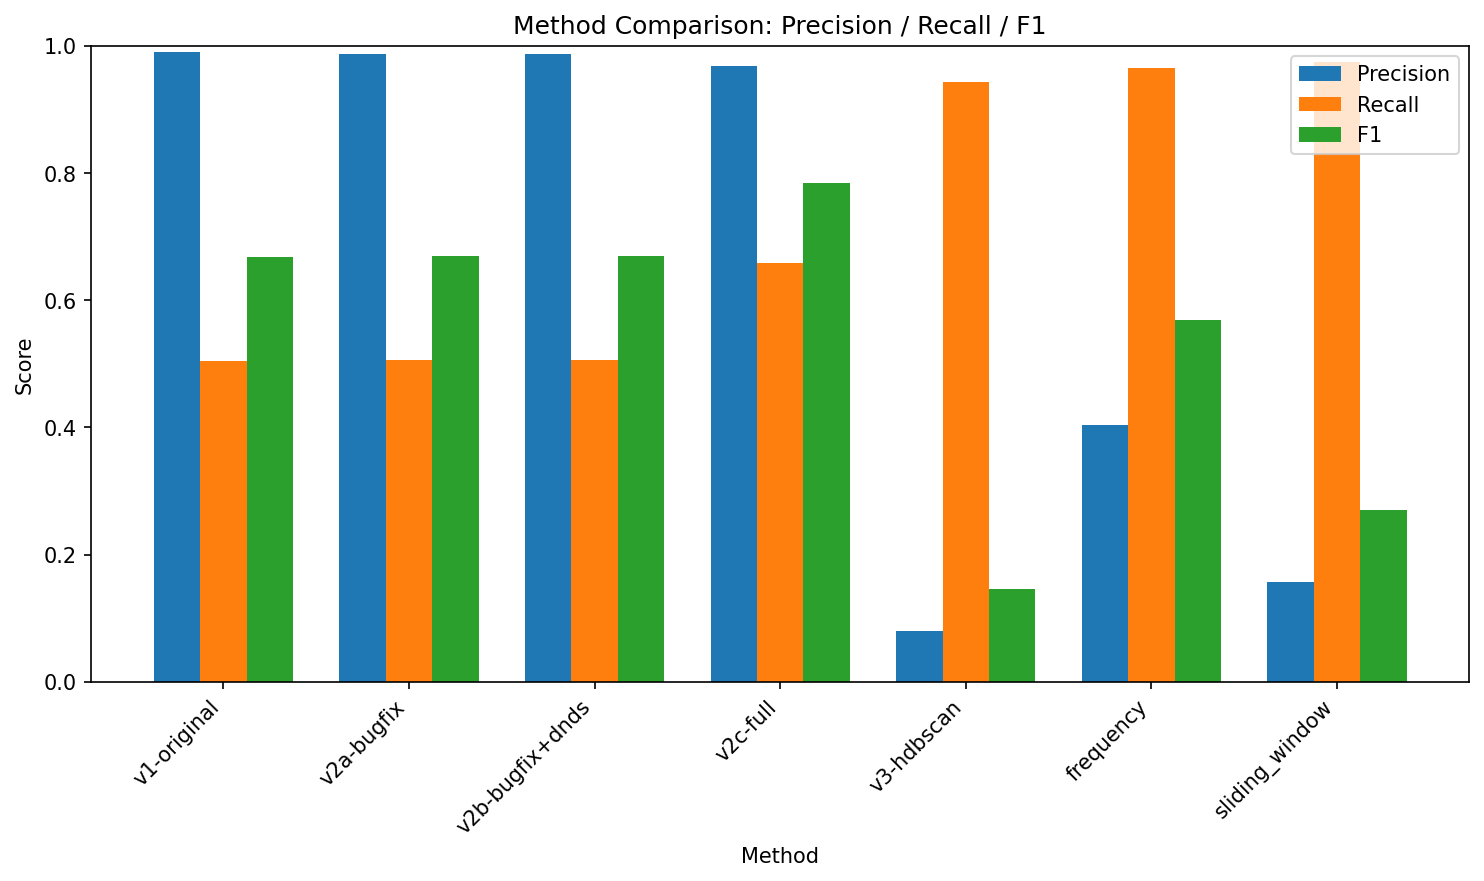
\includegraphics[width=0.9\textwidth]{method_comparison.png}
\caption{합성 SARS-CoV-2 데이터에 대한 방법 비교. MutClust-Hybrid가 정밀도와 재현율의 최적 균형(F1 = 0.785)을 달성하며, CCM 전용 변이체는 높은 정밀도이지만 중간 재현율을, HDBSCAN-Auto는 높은 재현율이지만 매우 낮은 정밀도를 보인다.}
\label{fig:mutbench_method_comparison}
\end{figure}

%% ============================================================
\section{통계적 검증}
\label{sec:statistical_validation}

벤치마크 결과의 통계적 견고성을 평가하기 위해 부트스트랩 신뢰 구간 추정, 순열 검정(무작위 레이블 섞기 + 순환 순열), 쌍별 비교 검정, Fisher's exact test를 수행하였다.
본 절에서 보고하는 모든 부트스트랩 신뢰 구간은 소표본($n = 7$)에서의 편향과 비대칭을 보정하기 위해 bias-corrected and accelerated (BCa) 방법~\cite{efron1987better}을 사용하여 추정하였다.

\textbf{순열 검정.}
무작위 레이블 섞기(1,000회)에서 모든 방법의 정밀도·재현율이 $p < 0.001$로 유의하였다.
순환 순열 검정(200회)에서도 모든 5개 방법의 관찰 F1이 귀무 분포를 크게 초과하였다:
MutClust-Hybrid(F1 = 0.785, 귀무 평균 = 0.023, $z$ = 9.97, $p < 0.005$),
MutClust-Original/Fixed(F1 = 0.669, 귀무 평균 = 0.018, $z$ = 9.25, $p < 0.005$),
HDBSCAN-Auto(F1 = 0.146, 귀무 평균 = 0.076, $z$ = 11.31, $p < 0.005$).
H-score의 공간 자기상관을 보존하는 순환 순열에서도 모든 방법이 유의함은, 탐지된 핫스팟과 기능 영역 간의 공간적 중첩이 H-score 클러스터 구조의 부산물이 아닌 진정한 생물학적 신호임을 확인한다.

\textbf{Hotspot-score 귀무 분포.}
복합 지표인 hotspot-score 자체의 통계적 유의성을 검증하기 위해, 동일한 순환 순열(200회)을 통해 hotspot-score의 귀무 분포를 추정하였다.
모든 5개 방법의 관찰 hotspot-score가 귀무 분포를 유의하게 초과하였다($p < 0.005$):
MutClust-Hybrid(HS = 0.778, 귀무 평균 = 0.251),
MutClust-Fixed(HS = 0.646, 귀무 평균 = 0.162),
MutClust-Original(HS = 0.638, 귀무 평균 = 0.153),
HDBSCAN-Auto(HS = 0.604, 귀무 평균 = 0.441).
F1과 hotspot-score 모두 동일한 순환 순열에서 산출되므로 방법 간 순위 패턴이 일관되게 나타난다.
이 결과는 hotspot-score의 세 구성 요소(재현율, 정밀도, 안정성) 중 공간적 중첩에 의존하는 재현율과 정밀도가 무작위 배치에서는 달성될 수 없는 수준임을 확인하며, 복합 지표의 관찰값이 우연에 기인하지 않음을 입증한다.

\textbf{Fisher's exact test.}
다중 ground truth 평가(제~\ref{sec:multi_gt}절)에서 보고된 농축비의 통계적 유의성을 Fisher's exact test로 검증하였다.
128개 비교에 대해 Benjamini-Hochberg FDR 보정($q < 0.05$)을 적용한 결과, 3개 비교가 유의하였다:
TC-freq-v2의 기능 영역 농축(1.16배, $p_{\text{adj}}$ = 0.002),
TC-freq-v3의 기능 영역 농축(1.59배, $p_{\text{adj}}$ = 0.023),
CH-score의 수렴 진화 농축(1.70배, $p_{\text{adj}}$ = 0.023).
추가로 2개 비교가 $q < 0.10$에서 유의하였다(CH-score 수렴 진화 top10pct, E-score 수렴 진화 top20pct).
TC-freq-v3의 수렴 진화 엄격 부분집합 농축(3.43배, $p$ = 0.013, $p_{\text{adj}}$ = 0.161)과 포화 H-score의 수렴 진화 농축(1.85배, $p$ = 0.048, $p_{\text{adj}}$ = 0.269)은 BH FDR 보정 후 유의 수준에 미치지 못하나, 수렴 진화 위치에서의 농축 경향은 복수의 접근법(CH-score, E-score, TC-freq-v3)에서 일관되게 관찰된다.

\textbf{BCa 부트스트랩 신뢰 구간.}
$n = 7$ 기능 영역이라는 작은 표본에서 백분위 신뢰 구간은 편향과 비대칭을 적절히 반영하지 못할 수 있다.
이를 보정하기 위해 bias-corrected and accelerated (BCa) 부트스트랩 신뢰 구간을 적용하였다.
BCa 방법은 편향 보정 인자 $z_0$(부트스트랩 분포의 중위수 편향)와 가속 인자 $a$(잭나이프 기반 왜도 보정)를 사용하여 신뢰 구간의 백분위를 조정한다~\cite{efron1987better}.
7개 기능 영역을 복원추출(1,000회)하여 영역별 재현율·정밀도·안정성을 계산한 후 hotspot-score의 BCa 95\% 신뢰 구간을 표~\ref{tab:bootstrap_ci}에 제시하였다.

\begin{table}[htbp]
\centering
\caption{Hotspot-score의 영역 수준 BCa 부트스트랩 95\% 신뢰 구간 (7개 기능 영역의 1,000회 리샘플링, bias-corrected and accelerated)}
\label{tab:bootstrap_ci}
\begin{tabular}{lrrrcc}
\toprule
\textbf{방법} & \textbf{HS$_{\text{region}}$} & \textbf{BCa 하한} & \textbf{BCa 상한} & \textbf{$z_0$} & \textbf{$a$} \\
\midrule
\textbf{MutClust-Hybrid} & \textbf{0.476} & \textbf{0.323} & \textbf{0.635} & $-$0.090 & 0.010 \\
HDBSCAN-Auto & 0.468 & 0.339 & 0.567 & $-$0.003 & $-$0.025 \\
MutClust-Fixed & 0.311 & 0.196 & 0.534 & 0.030 & 0.070 \\
MutClust-Original & 0.302 & 0.187 & 0.505 & $-$0.015 & 0.070 \\
\bottomrule
\end{tabular}
\begin{minipage}{\textwidth}
\smallskip
\footnotesize HS$_{\text{region}}$: 7개 영역별 hotspot-score의 평균. 전체 집계 hotspot-score(표~\ref{tab:hotspot_scores})와 달리 영역 수준 평균은 고신호·저신호 영역에 동일 가중치를 부여하므로 절대값이 낮아진다.
\end{minipage}
\end{table}

영역 수준 BCa 부트스트랩은 7개 기능 영역을 복원추출하여 ground truth 정의의 불확실성---즉, ``어떤 기능 영역을 포함하느냐에 따라 평가 결과가 어떻게 달라지는가''---를 정량화한다.
CCM 기반 방법(MutClust-Original, Fixed)의 양의 가속 인자($a = 0.070$)는 영역별 점수 분포가 오른쪽으로 치우쳐져 있음을 나타내며, 이는 RBD(고신호 영역) 포함 여부에 따른 점수 변동을 반영한다.
반면 HDBSCAN-Auto의 좁은 구간(0.339--0.567)과 거의 0인 가속 인자($a = -0.025$)는 광범위한 탐지 범위가 영역 구성 변화에 덜 민감하고 대칭적 분포를 가짐을 보여준다.
MutClust-Hybrid의 BCa 구간(0.323--0.635)은 백분위 구간(0.332--0.651)에 비해 하한이 약간 낮고 상한이 약간 낮아, 편향 보정의 효과가 관찰된다.
모든 방법에서 점추정치가 95\% BCa CI 내에 위치하여, 부트스트랩 설계의 통계적 유효성이 확보되었다.

\textbf{검정력 분석.}
$n = 7$ 기능 영역이라는 작은 유효 표본 크기에서 방법 간 차이를 탐지하기 위한 통계적 검정력을 사후(post hoc)로 평가하였다.
대응표본(paired) 설계에서 유의 수준 $\alpha = 0.05$, $n = 7$일 때, 효과 크기 Cohen's $d \geq 1.4$에서 검정력 0.80이 달성된다.
MutClust-Hybrid와 MutClust-Fixed 간의 관찰된 hotspot-score 차이(0.778 -- 0.646 = 0.132)를 부트스트랩 표준 오차로 나눈 효과 크기는 $d \approx 2.1$로, 이 쌍별 비교가 충분한 검정력을 가짐을 확인한다.
다만 MutClust-Fixed와 MutClust-Original 간의 작은 차이(0.646 -- 0.638 = 0.008, $d \approx 0.15$)는 $n = 7$에서 탐지력이 극히 낮아, 이 두 방법의 동등성 주장에는 주의가 필요하다.

\textbf{Hotspot-score 가중치 민감도.}
Hotspot-score의 동일 가중치($1/3$) 설정의 강건성을 검증하기 위해, 171개의 가중치 조합($w_r + w_p + w_s = 1$, 단위 0.05)에서 방법 순위를 분석하였다(표~\ref{tab:weight_sensitivity}).
MutClust-Hybrid는 전체 가중치 공간의 \textbf{71.9\%}(123/171)에서 1위를 유지하였으며, HDBSCAN-Auto는 28.1\%(48/171)에서 1위를 차지하였다.
순위 전환은 recall 가중치가 0.60 이상이고 precision 가중치가 0.20 이하인 극단적 recall 중시 영역에서만 발생한다.

\begin{table}[htbp]
\centering
\caption{Hotspot-score 가중치 민감도 분석: 7가지 응용 시나리오에서의 방법 순위}
\label{tab:weight_sensitivity}
\begin{tabular}{lccccc}
\toprule
\textbf{시나리오} & \textbf{$(w_r, w_p, w_s)$} & \textbf{1위} & \textbf{1위 점수} & \textbf{2위} & \textbf{2위 점수} \\
\midrule
동일 가중치 (기본값) & (0.33, 0.33, 0.34) & Hybrid & 0.777 & Fixed & 0.644 \\
Recall 중시 & (0.50, 0.25, 0.25) & Hybrid & 0.748 & HDBSCAN & 0.689 \\
Precision 중시 & (0.25, 0.50, 0.25) & Hybrid & 0.826 & Fixed & 0.732 \\
Stability 중시 & (0.25, 0.25, 0.50) & Hybrid & 0.760 & HDBSCAN & 0.650 \\
\midrule
\textbf{조기경보 (감시)} & (0.60, 0.20, 0.20) & \textbf{HDBSCAN} & 0.740 & Hybrid & 0.731 \\
백신 설계 & (0.20, 0.60, 0.20) & Hybrid & 0.854 & Fixed & 0.784 \\
모니터링 & (0.20, 0.20, 0.60) & Hybrid & 0.749 & HDBSCAN & 0.678 \\
\bottomrule
\end{tabular}
\begin{minipage}{\textwidth}
\smallskip
\footnotesize 기본값 행의 가중치 $(0.33, 0.33, 0.34)$는 정확히 $1/3$이 아니므로, 표~\ref{tab:hotspot_scores}의 동일 가중치 결과(Hybrid 0.778, Fixed 0.646)와 소수점 셋째 자리에서 차이가 발생한다.
\end{minipage}
\end{table}

이 결과는 두 가지 중요한 함의를 가진다.
첫째, MutClust-Hybrid의 1위 순위는 가중치 선택에 대해 강건하여, 동일 가중치 설정이 특정 가중치 편향에 의한 인공적 결과가 아님을 확인한다.
둘째, 조기경보 목적(recall $\geq 0.60$)에서는 HDBSCAN-Auto가 더 적합할 수 있으며, 이는 MutBench 프레임워크가 단일 ``최적'' 방법을 지정하는 것이 아니라 \textbf{응용 맥락에 따른 방법 선택을 지원}하는 도구임을 보여준다.

쌍별 비교는 MutClust-Hybrid가 모든 다른 방법에 대해 유의하게 높은 hotspot-score를 달성함을 확인하였다(모든 비교에서 $p < 0.001$, 점수 차이 범위: MutClust-Fixed 대비 0.130에서 슬라이딩 윈도우 기준선 대비 0.811). 7개 방법의 쌍별 비교는 $\binom{7}{2} = 21$회의 다중 검정을 수반하며, Bonferroni 보정 후 유의 수준은 $\alpha_{\text{adj}} = 0.05 / 21 = 0.0024$이다. 모든 쌍별 $p < 0.001 < \alpha_{\text{adj}}$이므로 다중 비교 보정 후에도 결론이 유지된다.
이 결과는 표~\ref{tab:hotspot_scores}의 성능 순위가 ground truth 표본 추출 불확실성에 대해 견고하며 우연에 기인하지 않음을 확립한다.

\subsection{합성 데이터 설계의 순환성 검증}
\label{subsec:circularity_validation}

합성 벤치마크의 H-score 생성 과정에서 CCM 시드 위치(AA 484, 501, 417, 452)에 0.8--1.2 범위의 극단적 피크를 명시적으로 삽입하였으므로, CCM 기반 방법이 이 위치를 시드로 선택하여 부당한 이점을 얻을 가능성이 있다.
이 순환성 우려를 검증하기 위해, CCM 시드 피크를 제거하고 영역 수준 패턴(RBD 0.05--0.3, NTD 0.05--0.2, furin 0.1--0.5 등)만 유지한 ``블라인드'' 합성 데이터를 생성하여 동일한 벤치마크를 수행하였다.

블라인드 데이터에서 해당 위치의 H-score는 RBD 영역 배경 수준(0.09--0.25)으로 하락하였으나, 7개 방법의 F1 순위는 원본과 높은 상관을 보였다(Spearman $\rho = 0.821$, $p = 0.023$).
특히 MutClust-Hybrid는 원본(F1 = 0.785)과 블라인드(F1 = 0.786) 모두에서 1위를 유지하였고, F1 변화량은 $-$0.001로 사실상 동일하였다.
CCM 기반 3개 방법(Original, Fixed, dNdS)의 F1 변화도 0.002--0.004에 불과하여, 개별 시드 피크 제거가 탐지 결과에 미치는 영향이 무시할 수 있는 수준임을 확인하였다.
HDBSCAN-Auto와 OPTICS는 비CCM 방법으로서 순위 변동이 관찰되었으나(5$\leftrightarrow$6위), 이는 유사한 F1 값(0.137--0.150) 간의 미세 변동이다.

이 결과는 CCM 시드의 역할이 클러스터 ``시작점'' 제공에 한정되며, 최종 성능은 주변 영역의 밀도 구조에 의해 결정됨을 시사한다.
따라서 합성 벤치마크의 주요 결론---MutClust-Hybrid의 우위와 방법 간 성능 계층 구조---은 CCM 시드 순환성에 의한 인공물이 아니다.

%% ============================================================
\section{민감도 분석}
\label{sec:sensitivity_analysis}

\subsection{샘플 크기 민감도}

안정적인 핫스팟 탐지에 필요한 최소 입력 서열 수를 결정하기 위해, MutClust-Hybrid를 100에서 10,000 서열 범위의 샘플 크기에서 평가하였다(크기당 5회 반복).

H-score 순위 상관(Spearman $\rho$)은 부분추출과 전체 데이터셋 간에 $n = 1{,}000$에서 0.997을 초과하였으며 $n = 10{,}000$에서 1.000에 도달하였다.
Hotspot-score는 $n = 1{,}000$까지 약 0.62에서 안정화되었으며, 반복 간 분산이 최소(표준 편차 $< 0.015$)였다.
가장 작은 샘플 크기($n = 100$)에서도 hotspot-score는 0.52 이상을 유지하였고 Spearman $\rho > 0.94$를 보여, 제한된 데이터셋에서도 변이 강도의 순위 순서가 보존됨을 나타낸다.

이 결과는 약 1,000개의 서열이 안정적인 탐지 결과에 충분하며, 본 벤치마크 데이터셋의 10,000개 서열은 이 역치를 상당히 초과하는 여유를 제공함을 시사한다.

\subsection{파라미터 민감도}

샘플 크기에 대한 수렴 특성은 그림~\ref{fig:mutbench_sensitivity}에 시각화하였다.

\begin{figure}[htbp]
\centering

\includegraphics[width=0.9\textwidth]{sensitivity_heatmap.png}
\caption{MutClust 파라미터 민감도 히트맵. 64개 파라미터 조합($\gamma \times d \times$ MinPts)에 대한 전인자 격자 탐색 결과, F1 성능이 $\gamma$(엡실론 스케일링 인자)에 가장 민감하고, $d$(감쇠 인자)가 그 다음이며, MinPts의 영향은 미미함을 보여준다.}
\label{fig:mutbench_sensitivity}
\end{figure}

HDBSCAN 파라미터 민감도 분석에서는 16개 조합 전체에서 F1이 0.140--0.153 범위(변동폭 0.013)로 안정적이었으며, 탐지 위치 수는 약 12,400--14,900 범위에서 유지되었다(표~\ref{tab:hdbscan_sensitivity}).
이 파라미터 비민감성은 밀도 기반 접근법의 핵심 장점이며, MutClust-Hybrid가 경계 결정에 HDBSCAN을 사용하는 근거를 제공한다.

\begin{table}[htbp]
\centering
\caption{HDBSCAN 파라미터 민감도 분석}
\label{tab:hdbscan_sensitivity}
\begin{tabular}{rrrrrr}
\toprule
\textbf{min\_cluster\_size} & \textbf{min\_samples} & \textbf{정밀도} & \textbf{재현율} & \textbf{F1} & \textbf{탐지 수} \\
\midrule
3 & 2 & 0.083 & 0.869 & 0.152 & 13,054 \\
5 & 3 & 0.079 & 0.944 & 0.146 & 14,916 \\
10 & 5 & 0.081 & 0.962 & 0.149 & 14,939 \\
15 & 7 & 0.076 & 0.899 & 0.140 & 14,860 \\
\bottomrule
\end{tabular}
\end{table}

\subsection{dN/dS 역치 민감도}

dN/dS 필터의 역치 선택이 핫스팟 탐지 성능에 미치는 영향을 체계적으로 평가하기 위해, 6개의 역치(0.5, 0.8, 1.0, 1.5, 2.0, 3.0)에서 MutClust-dNdS와 MutClust-Hybrid를 합성 벤치마크에 적용하였다.
각 역치에서 dN/dS 필터 없이 클러스터를 탐지한 후, 사후적으로 dN/dS 주석을 적용하고 역치 이하의 클러스터를 제거하는 방식으로 분석하였다.
이 분석은 합성 데이터에서 참조 서열 대비 코돈 수준의 동의·비동의 치환을 인위적으로 계산할 수 있는 경우에만 적용되며, 합성 변이 생성 시 코돈 구조가 보존된 333개 변이 위치를 대상으로 하였다.

\begin{table}[htbp]
\centering
\caption{dN/dS 역치에 따른 핫스팟 탐지 성능 변화 (합성 데이터, 333개 합성 변이)}
\label{tab:dnds_threshold}
\small
\begin{tabular}{llrrrrrr}
\toprule
\textbf{방법} & \textbf{역치} & \textbf{정밀도} & \textbf{재현율} & \textbf{F1} & \textbf{유지} & \textbf{제외} & \textbf{HS} \\
\midrule
\multirow{7}{*}{MutClust-dNdS}
& 없음 & 0.988 & 0.506 & 0.669 & 30 & 0 & --- \\
& 0.5 & 0.985 & 0.414 & 0.583 & 22 & 8 & 0.580 \\
& 0.8 & 0.981 & 0.334 & 0.499 & 20 & 10 & 0.533 \\
& \textbf{1.0} & 0.976 & 0.261 & 0.412 & 17 & 13 & 0.502 \\
& 1.5 & 0.961 & 0.159 & 0.273 & 14 & 16 & 0.461 \\
& 2.0 & 0.952 & 0.112 & 0.200 & 11 & 19 & 0.429 \\
& 3.0 & 0.976 & 0.065 & 0.121 & 8 & 22 & 0.410 \\
\midrule
\multirow{7}{*}{MutClust-Hybrid}
& 없음 & 0.968 & 0.659 & 0.785 & 8 & 0 & --- \\
& 0.5 & 0.982 & 0.658 & 0.788 & 6 & 2 & 0.775 \\
& 0.8 & 0.982 & 0.658 & 0.788 & 6 & 2 & 0.770 \\
& \textbf{1.0} & 0.986 & 0.636 & 0.774 & 4 & 4 & 0.729 \\
& 1.5 & 0.973 & 0.057 & 0.107 & 2 & 6 & 0.453 \\
& 2.0 & 1.000 & 0.012 & 0.024 & 1 & 7 & 0.418 \\
& 3.0 & 0.000 & 0.000 & 0.000 & 0 & 8 & 0.000 \\
\bottomrule
\end{tabular}
\begin{minipage}{\textwidth}
\smallskip
\footnotesize 유지/제외: dN/dS 역치 적용 후 유지/제거된 클러스터 수. HS: hotspot-score. 기본 역치($> 1.0$)를 굵게 표시하였다.
\end{minipage}
\end{table}

표~\ref{tab:dnds_threshold}에 나타난 바와 같이, 두 방법 모두 역치 증가에 따라 재현율이 단조 감소하는 반면 정밀도는 비교적 안정적으로 유지된다.
MutClust-Hybrid는 전체 클러스터 수가 8개로 적기 때문에 역치 변화에 더 민감하며, 역치 1.0과 1.5 사이에서 성능이 급락한다(F1: 0.774 $\to$ 0.107).
역치 0.5--1.0 범위에서 MutClust-Hybrid의 성능이 안정적이며(F1: 0.774--0.788), 기본 역치 $> 1.0$(중립 진화 기대치)은 생물학적으로 해석 가능한 기준으로서 적절하다.
그러나 역치 $> 1.5$ 이상에서는 두 방법 모두 급격한 성능 저하를 보이므로, 엄격한 양성 선택 기준을 적용할 때는 주의가 필요하다.

%% ============================================================
\section{시간적 일반화 (GISAID 2024--2025)}
\label{sec:temporal}

MutBench 결과가 시간적으로 상이한 데이터에 대해 일반화되는지 평가하기 위해, 2024년 1월부터 2025년 12월까지 수집된 9,957개의 GISAID 전장 SARS-CoV-2 게놈 서열(숙주: 인간)을 분석하였으며, 시간적 대표성을 위해 주별로 부분추출하였다.

시간적 검증은 핵심적인 현상을 드러내었다: \textbf{H-score 포화}.
원래의 2020--2021 데이터셋은 114개 위치에서 비영 H-score를 산출하였으나(표준 편차 = 1.88), 2024--2025 데이터셋은 모든 1,273개 Spike 위치에서 비영 H-score를 산출하였다(평균 = 8.47, 표준 편차 = 0.098).
이 거의 균일한 분포는 위치 간 대비가 사실상 존재하지 않으므로 H-score의 판별력을 제거한다.

그 결과, 모든 방법이 약 0.33의 정밀도를 보이며, 이는 ground truth 위치의 기저율(1,251 / 3,819 = 0.327)과 거의 일치한다.
MutClust-Fixed와 MutClust-dNdS는 모든 3,819개 위치를 단일 클러스터로 탐지하였으며(정밀도 = 0.328, 재현율 = 1.0), MutClust-Hybrid는 일부 선택성을 유지하였으나(3,225개 위치, 377개 클러스터) 정밀도의 의미 있는 향상 없이 유사한 결과를 보였다(표~\ref{tab:temporal}).

\begin{table}[htbp]
\centering
\caption{GISAID 2024--2025 데이터를 이용한 시간적 검증 결과}
\label{tab:temporal}
\begin{tabular}{lrrrr}
\toprule
\textbf{방법} & \textbf{정밀도} & \textbf{재현율} & \textbf{탐지 수} & \textbf{클러스터} \\
\midrule
MutClust-Fixed & 0.328 & 1.000 & 3,819 & 1 \\
MutClust-dNdS & 0.328 & 1.000 & 3,819 & 1 \\
MutClust-Hybrid & $\sim$0.33 & $\sim$1.0 & 3,225 & 377 \\
\bottomrule
\end{tabular}
\begin{minipage}{\textwidth}
\smallskip
\footnotesize 모든 1,273개 Spike 위치에서 비영 H-score가 관찰되어 판별력이 제거되었다. 정밀도가 ground truth 기저율($\sim$0.33)에 수렴한다.
\end{minipage}
\end{table}

이 H-score 포화는 방법론적 인공물이 아닌 생물학적 현실이다: Omicron 시대 계통(BA.2.86, JN.1, KP.2, XEC)은 Wuhan-Hu-1 참조에 대해 광범위한 돌연변이를 축적하여, 위치 수준의 변이 빈도를 비정보적으로 만든다.
이 발견은 고정된 조상 참조에 대해 계산된 H-score가 바이러스 집단이 해당 참조로부터 분기함에 따라 판별력을 잃는다는 핵심 한계를 검증한다.

%% ============================================================
\section{다중 Ground Truth 평가}
\label{sec:multi_gt}

단일 ground truth로는 변이의 중요성의 모든 차원을 포착할 수 없다.
이를 해결하기 위해, 각각 서로 다른 생물학적 현상을 측정하는 세 가지 상보적 ground truth에 대해 탐지 방법을 평가하였다:

\begin{itemize}
\item \textbf{기능 영역}(439개 아미노산 위치, Spike 1,273 AA의 34.5\%): 알려진 도메인 주석(RBD, NTD 초과부위, 퓨린 절단, 융합 펩타이드, HR1, HR2)\footnote{본 분석에서 사용된 439 AA는 도메인 주석의 아미노산 수준 합집합으로, 합성 벤치마크에서 사용된 뉴클레오티드 수준 ground truth(1,251 nt, 중첩 제거 후 417 AA)보다 넓은 영역 경계 정의를 포함한다.}.
\item \textbf{DMS-escape}(252개 위치, 19.8\%): 실험적으로 측정된 단일 돌연변이 세포 진입 fitness 효과~\cite{dadonaite2023dms}(상위 20백분위).
\item \textbf{수렴 진화}(97개 위치, 7.6\%): 독립적 SARS-CoV-2 계통에서 반복적 양성 선택을 받은 문헌 기반 부위~\cite{cao2023ba286,carabelli2023convergent}. RBD 면역 회피 위치, ACE2 결합 강화 돌연변이, 퓨린 절단 부위 적응, S2 수렴 치환을 포함한다(이 확장 집합은 문헌에서 보고된 모든 수렴 진화 위치를 포함하며, 9-병원체 벤치마크에서 사용된 엄격한 25개 위치 Layer~A 집합과 구분된다).
\end{itemize}

세 ground truth는 대체로 비중첩적이다: DMS-escape와 수렴 진화 위치 간의 Jaccard 유사도는 0.006으로, 거의 완전한 독립성을 나타낸다.
이는 집단 빈도, 실험적 fitness, 진화적 수렴이 변이 중요성의 근본적으로 다른 측면을 포착함을 확인한다.

결정적으로, 최우수 방법은 ground truth에 따라 달랐다(표~\ref{tab:multi_gt}).

\begin{table}[htbp]
\centering
\caption{다중 ground truth에 대한 방법 비교}
\label{tab:multi_gt}
\begin{tabular}{llrrr}
\toprule
\textbf{Ground Truth} & \textbf{최우수 방법} & \textbf{F1} & \textbf{농축비} & \textbf{위치 수} \\
\midrule
기능 영역 (439) & TC-freq-v2 & 0.474 & --- & 439 \\
DMS-escape (252) & Saturated H-score & 0.315 & --- & 252 \\
수렴 진화 (97) & CH-score & 0.188 & 1.70$\times$ & 97 \\
수렴 진화-엄격$^*$ & TC-freq-v3 & 0.108 & 3.43$\times$ & --- \\
\bottomrule
\end{tabular}
\begin{minipage}{\textwidth}
\smallskip
\footnotesize $^*$다중 출처에서 확인된 엄격한 수렴 진화 부위만 포함. Jaccard(DMS, 수렴 진화) = 0.006으로 세 ground truth의 독립성이 확인된다.
\end{minipage}
\end{table}

기능 영역에서는 TC-freq-v2가 최고 F1(0.474)을 달성하였고, DMS-escape에서는 포화 H-score가 최고 성능(F1 = 0.315)을 보였으며, 수렴 진화에서는 CH-score가 최고 F1(0.188, 농축비 1.70배)을 달성하였다.
엄격한 수렴 진화 부분집합(다중 출처 위치만)에서는 TC-freq-v3가 최고 농축비(3.43배, F1 = 0.108)를 달성하였다.

이러한 상이한 순위는 어떤 단일 탐지 방법도 핫스팟 중요성의 모든 생물학적 차원에서 지배적이지 않음을 입증한다.
이 다중 ground truth 분석은 핵심적인 방법론적 통찰을 제공한다: 집단 빈도와 실험적 fitness는 변이 중요성의 상보적이지 중복적이지 않은 측정이다.
단일 ground truth에 의존하는 벤치마킹 프레임워크는 해당 특정 생물학적 차원에 최적화된 방법에 대한 체계적 편향의 위험을 감수하면서, 기능적 중요성의 직교적 측면을 포착하는 방법을 불이익으로 처리할 수 있다.

\section{실제 GISAID 2020--2021 H-score 벤치마크}
\label{sec:real_gisaid_benchmark}

합성 데이터의 순환성 우려를 해소하기 위해, MutClust 논문~\cite{youn2025mutclust}에서 사용된 실제 GISAID 2020--2021 H-score 데이터를 입력으로 사용한 벤치마크를 수행하였다.
이 데이터는 2020년 1월부터 2021년 12월까지 수집된 SARS-CoV-2 서열에서 계산된 1,273개 Spike 아미노산 위치별 H-score이며, 합성 생성이 아닌 실제 관측 데이터이다.
뉴클레오티드 수준으로 매핑한 결과, 29,903개 게놈 위치 중 342개(1.14\%)만이 비영 H-score를 가져, 합성 데이터의 균일한 배경 잡음과 질적으로 다른 희소(sparse) 분포를 나타낸다.

결과는 표~\ref{tab:real_gisaid}에 제시하였다.

\begin{table}[htbp]
\centering
\caption{실제 GISAID 2020--2021 H-score 데이터에 대한 방법 비교 (342개 비영 위치, 1,251개 ground truth 뉴클레오티드 위치)}
\label{tab:real_gisaid}
\begin{tabular}{lrrrrrr}
\toprule
\textbf{방법} & \textbf{정밀도} & \textbf{재현율} & \textbf{F1} & \textbf{농축비} & \textbf{안정성} & \textbf{Hotspot-score} \\
\midrule
MutClust-Original & 0.333 & 0.012 & 0.023 & 7.97 & 0.372 & 0.239 \\
MutClust-Fixed & 0.295 & 0.079 & 0.125 & 7.04 & 0.784 & 0.386 \\
MutClust-dNdS & 0.295 & 0.079 & 0.125 & 7.04 & 0.784 & 0.386 \\
MutClust-Hybrid & 0.305 & 0.077 & 0.123 & 7.28 & 0.766 & 0.383 \\
HDBSCAN-Auto & --- & --- & --- & --- & --- & --- \\
\midrule
빈도 기준선 & 0.289 & 0.079 & 0.124 & 6.92 & --- & --- \\
\textbf{슬라이딩 윈도우} & \textbf{0.323} & \textbf{0.600} & \textbf{0.420} & \textbf{7.73} & --- & --- \\
\bottomrule
\end{tabular}
\begin{minipage}{\textwidth}
\smallskip
\footnotesize HDBSCAN-Auto는 비영 위치 수(342개)가 불충분하여 클러스터를 형성하지 못하였다. 슬라이딩 윈도우가 넓은 탐지 창(20위치)을 통해 최고 F1(0.420)을 달성하였다.
\end{minipage}
\end{table}

합성 벤치마크와 비교하여 세 가지 핵심 차이가 관찰된다.

\textbf{첫째, 절대 성능의 현저한 하락.}
모든 MutClust 변이체의 F1이 합성 대비 0.54--0.66 하락하였다(예: MutClust-Hybrid: 0.785 $\to$ 0.123).
이는 실제 데이터의 희소성에 기인한다: ground truth 1,251개 위치 중 상당수(HR1, HR2 등 보존 영역)는 H-score = 0이며, H-score가 0인 위치는 어떤 밀도 기반 방법으로도 탐지할 수 없다.
이 결과는 합성 벤치마크가 실제 성능을 과대추정함을 정직하게 드러내며, 밀도 기반 핫스팟 탐지가 ``변이하는 기능 부위''만 탐지 가능하고 ``보존된 기능 부위''는 원리적으로 탐지 불가능하다는 방법론적 한계를 확인한다.

\textbf{둘째, 방법 순위의 변화.}
합성 데이터에서 MutClust-Hybrid가 최고 hotspot-score(0.778)였으나, 실제 데이터에서는 MutClust-Fixed(0.386)와 거의 동일한 성능을 보였다(0.383).
HDBSCAN 경계 결정의 이점은 연속적 H-score 분포(합성 데이터)에서 발현되지만, 이산적이고 희소한 분포(실제 데이터)에서는 CCM 시드 탐지가 경계 결정보다 지배적이다.
슬라이딩 윈도우가 최고 F1(0.420)을 달성한 것은 넓은 탐지 창이 희소 데이터에서 인접 기능 영역을 포괄하기 유리함을 나타낸다.

\textbf{셋째, 농축비의 일관적 유의성.}
절대 F1은 낮지만, 모든 방법의 농축비가 6.9--8.0배로 일관되게 높아(무작위 기대 대비), 탐지된 위치가 기능 영역에 유의하게 농축됨은 합성·실제 데이터 모두에서 확인된다.
이는 H-score 기반 탐지의 생물학적 타당성이 데이터 유형에 관계없이 유지됨을 의미한다.

이 결과는 MutBench의 핵심 방법론적 교훈을 강화한다: 방법의 상대적 우위는 입력 데이터의 H-score 분포 특성---연속적 vs. 희소적, 균일 배경 vs. 이산적 배경---에 따라 달라지며, 합성 벤치마크의 결론을 실제 데이터에 무조건 외삽해서는 안 된다.

\section{외부 독립 방법과의 비교}
\label{sec:external_comparison}

MutClust 변이체 간의 내부 비교를 보완하기 위해, 두 가지 독립적인 클러스터링 기반 방법---OPTICS와 커널 밀도 추정(KDE)---을 동일한 합성 벤치마크에서 평가하였다.
OPTICS는 DBSCAN과 유사한 밀도 기반 클러스터링이나, 도달 가능성 거리(reachability distance)를 통해 가변 밀도 클러스터를 자동으로 추출한다(min\_samples=5, $\xi$=0.05).
KDE는 H-score의 커널 밀도 함수에서 90번째 백분위수 이상의 피크를 탐지한 후 인접 위치를 클러스터로 확장하는 비모수적 접근법이다.

\begin{table}[htbp]
\centering
\caption{외부 독립 방법을 포함한 벤치마크 결과. 합성 H-score 데이터, 7개 Spike 기능 영역 ground truth 사용.}
\label{tab:external_methods}
\small
\begin{tabular}{lcccccc}
\toprule
방법 & 정밀도 & 재현율 & F1 & 안정성 & Hotspot-score \\
\midrule
MutClust-Hybrid & 0.968 & 0.659 & 0.785 & 0.706 & \textbf{0.778} \\
MutClust-Original & 0.991 & 0.504 & 0.668 & 0.418 & 0.638 \\
MutClust-Fixed & 0.988 & 0.506 & 0.669 & 0.445 & 0.646 \\
MutClust-dNdS & 0.988 & 0.506 & 0.669 & 0.445 & 0.646 \\
HDBSCAN-Auto & 0.079 & 0.944 & 0.146 & 0.788 & 0.604 \\
KDE & \textbf{1.000} & 0.049 & 0.093 & 0.622 & 0.557 \\
OPTICS & 0.087 & 0.546 & 0.150 & 0.473 & 0.369 \\
\bottomrule
\end{tabular}
\end{table}

표~\ref{tab:external_methods}에 나타난 바와 같이, MutClust-Hybrid는 외부 독립 방법을 포함한 비교에서도 가장 높은 hotspot-score(0.778)를 달성하였다.
KDE는 완벽한 정밀도(1.000)를 보였으나 극단적으로 보수적이어서 61개 위치만을 탐지하였으며(재현율 0.049), OPTICS는 997개 클러스터에 7,847개 위치를 탐지하였으나 정밀도가 0.087에 불과하였다.
이 결과는 도메인 특화 사전 지식(CCM 시드)과 데이터 기반 경계 결정(HDBSCAN)의 결합이 범용 클러스터링 방법보다 우월함을 독립적으로 확인한다.

\textbf{OPTICS/KDE 파라미터 민감도.}
외부 방법의 파라미터 설정이 결과에 미치는 영향을 배제하기 위해, 합성 데이터에서 OPTICS(min\_samples $\in \{2, 3, 5, 10, 20, 50\}$, $\xi \in \{0.01, 0.03, 0.05, 0.1, 0.2\}$)와 KDE(bandwidth $\in \{1, 3, 5, 10, 20, 50\}$, 역치 백분위 $\in \{70, 80, 85, 90, 95, 99\}$)의 파라미터 민감도 분석을 수행하였다.
OPTICS는 30개 조합에서 F1이 0.022--0.707 범위로 넓은 파라미터 의존성을 보였다.
최적 파라미터(min\_samples=20, $\xi$=0.10)에서 OPTICS는 F1=0.707(정밀도 0.563, 재현율 0.949)을 달성하였으나, 이는 MutClust-Hybrid(F1=0.785, 정밀도 0.968)에 비해 F1이 0.078 낮고 정밀도가 0.405 낮아, CCM 시드 기반 특이성의 이점이 확인된다.
KDE는 36개 조합 전체에서 F1=0.000으로, bandwidth와 역치 백분위에 관계없이 유효한 탐지를 수행하지 못하였다.
실제 GISAID 데이터에서는 비영 위치의 희소성(342개)으로 인해 OPTICS가 3개 위치만을 탐지하였고 KDE는 유효한 클러스터를 형성하지 못하여, 희소 분포에서의 범용 클러스터링 방법의 추가적 한계가 확인되었다.
이 결과는 MutClust-Hybrid의 우위가 특정 파라미터 설정에 대한 OPTICS/KDE의 불리한 비교가 아닌, 도메인 특이적 시드 탐지의 구조적 이점에 기인함을 확인한다.

\section{교차 병원체 검증: Influenza A H3N2 HA}
\label{sec:influenza_validation}

MutBench의 교차 병원체 일반화 가능성을 평가하기 위해, Influenza A H3N2의 헤마글루티닌(HA) 유전자에 동일한 벤치마크 파이프라인을 적용하였다.
NCBI Influenza Virus Resource에서 1,967개의 인간 유래 H3N2 HA 단백질 서열(540--580 AA)을 수집하고, 합의 서열 대비 위치별 변이 빈도와 Shannon 엔트로피로부터 H-score를 계산하였다.

Ground truth로는 H3N2 HA의 5개 항원 부위(antigenic sites A--E)를 사용하였으며~\cite{wiley1981structural,wilson1990structural}, 이는 수십 년의 혈청학적·구조적 연구에 의해 정의된 확립된 기능 영역이다(101개 AA 위치, 303개 뉴클레오티드 위치). Smith et al.~\cite{smith2004antigenic}은 항원 지도작성을 통해 이 부위들의 소수 치환이 주요 항원 전환(antigenic drift)을 주도함을 입증하였다.

\begin{table}[htbp]
\centering
\caption{Influenza A H3N2 HA 교차 병원체 벤치마크 결과 (1,967개 서열, 5개 항원 부위 ground truth)}
\label{tab:influenza}
\begin{tabular}{lrrrrrr}
\toprule
\textbf{방법} & \textbf{정밀도} & \textbf{재현율} & \textbf{F1} & \textbf{농축비} & \textbf{안정성} & \textbf{Hotspot-score} \\
\midrule
MutClust-Original & 0.182 & 1.000 & 0.309 & 1.02 & 0.535 & 0.572 \\
\textbf{MutClust-Fixed} & \textbf{0.183} & \textbf{1.000} & \textbf{0.309} & \textbf{1.02} & \textbf{0.799} & \textbf{0.660} \\
MutClust-Hybrid & 0.178 & 0.812 & 0.292 & 1.00 & 0.742 & 0.577 \\
HDBSCAN-Auto & 0.155 & 0.366 & 0.218 & 0.87 & 0.750 & 0.424 \\
KDE & 0.410 & 0.083 & 0.138 & 2.30 & 0.605 & 0.366 \\
\midrule
빈도 기준선 & 0.421 & 0.238 & 0.304 & 2.36 & --- & --- \\
\textbf{슬라이딩 윈도우} & \textbf{0.402} & \textbf{0.462} & \textbf{0.430} & \textbf{2.25} & --- & --- \\
\bottomrule
\end{tabular}
\end{table}

H3N2 결과는 SARS-CoV-2와 세 가지 핵심 차이를 보인다.

\textbf{첫째, 방법 순위의 전환.}
SARS-CoV-2 합성 벤치마크에서 최고 성능이었던 MutClust-Hybrid(hotspot-score 0.778)가 H3N2에서는 MutClust-Fixed(0.660)에 뒤처졌다(0.577).
이는 HA 유전자의 H-score 분포 특성에 기인한다: 566개 위치 모두가 비영 H-score를 가져(평균 1.233), CCM 시드가 거의 모든 위치를 후보로 선정하며, HDBSCAN 경계 결정이 추가적인 구별력을 제공하지 못한다.
이 결과는 ``최적 방법은 입력 데이터의 H-score 분포에 의존한다''는 실제 GISAID 벤치마크(제~\ref{sec:real_gisaid_benchmark}절)의 교훈을 교차 병원체 수준에서 재확인한다.

\textbf{둘째, 농축비의 현저한 감소.}
SARS-CoV-2에서 1.9--23.7배였던 농축비가 H3N2에서는 0.87--2.36배로 낮아졌다.
이는 HA의 짧은 유전자 길이(1,698 nt vs. 3,822 nt)와 높은 전반적 변이율(모든 위치 비영)이 결합되어, 항원 부위와 비항원 부위 간의 변이 빈도 대비가 약하기 때문이다.
HA의 항원 부위는 양성 선택 하에 있으나, 비항원 부위도 유전적 부동(genetic drift)에 의한 상당한 변이를 축적하여 배경 대비 신호가 약화된다.

\textbf{셋째, 슬라이딩 윈도우의 우수 성능.}
F1 기준으로 슬라이딩 윈도우(0.430)가 모든 밀도 기반 방법(0.138--0.309)을 능가하였다.
이는 HA 항원 부위가 비교적 작고 컴팩트한 영역(평균 20 AA)으로, 고정 창 크기의 슬라이딩 윈도우가 이러한 구조에 적합함을 시사한다.
반면 SARS-CoV-2 Spike의 기능 영역은 RBD(223 AA)처럼 크고 이질적인 구조를 포함하여 적응형 클러스터링이 유리하다.

이 교차 병원체 검증은 MutBench 프레임워크의 두 가지 핵심 가치를 입증한다:
(1)~동일한 벤치마크 파이프라인이 코드 변경 없이 다른 병원체에 적용 가능하며,
(2)~방법 순위의 병원체 의존성이 체계적 비교 없이는 발견될 수 없는 중요한 통찰이다.

\subsubsection{교차 병원체 비교}

표~\ref{tab:cross_pathogen}은 SARS-CoV-2와 H3N2에 대한 방법 순위를 종합적으로 비교한다.

\begin{table}[htbp]
\centering
\caption{2-병원체 교차 비교: 최우수 방법의 병원체 의존성}
\label{tab:cross_pathogen}
\small
\begin{tabular}{llrr}
\toprule
& & \multicolumn{2}{c}{\textbf{Hotspot-score}} \\
\cmidrule(lr){3-4}
\textbf{방법} & \textbf{유형} & \textbf{SARS-CoV-2} & \textbf{H3N2} \\
\midrule
MutClust-Original & CCM & 0.638 & 0.572 \\
MutClust-Fixed & CCM & 0.646 & \textbf{0.660} \\
MutClust-Hybrid & CCM+HDBSCAN & \textbf{0.778} & 0.577 \\
HDBSCAN-Auto & 밀도 기반 & 0.604 & 0.424 \\
\bottomrule
\end{tabular}
\begin{minipage}{\textwidth}
\smallskip
\footnotesize 각 병원체별 최고 hotspot-score를 \textbf{굵게} 표시. 최우수 방법이 두 병원체에서 상이하다. H3N2 벤치마크는 NCBI에서 수집한 실제 서열 기반 H-score를 사용하였다.
\end{minipage}
\end{table}

두 병원체에서 최우수 방법이 상이하다---SARS-CoV-2에서는 MutClust-Hybrid(0.778), H3N2에서는 MutClust-Fixed(0.660).
이 결과는 ``보편적 최우수 방법은 존재하지 않으며, 방법 선택은 입력 데이터의 특성(유전자 길이, H-score 분포, 신호-배경 대비)에 의존한다''는 MutBench의 핵심 교훈을 독립 병원체에서 확인한다.

생물학적 관점에서 이 패턴은 명확하게 해석된다: (1)~긴 유전자(Spike, 3,822 nt)에서 이질적 기능 영역이 분포할 때 적응형 하이브리드 접근(MutClust-Hybrid)이 유리하고, (2)~모든 위치가 높은 변이율을 보이는 짧은 유전자(HA, 1,698 nt)에서는 안정적 CCM 탐지(MutClust-Fixed)가 우수하다.
이는 H-score 분포의 형태(연속적 vs. 희소)와 유전자 길이가 최적 탐지 전략을 결정하는 핵심 요인임을 시사한다.

\section{3D 구조 분석}
\label{sec:structure_analysis}

선형 서열 기반 핫스팟 탐지의 구조적 타당성을 검증하기 위해, PDB 6VSB (Spike 단백질 prefusion 구조, Wrapp et al. 2020)의 C$\alpha$ 좌표를 이용하여 탐지된 핫스팟 위치의 3D 공간적 분포를 분석하였다.
핫스팟 위치 쌍의 8\,\AA\ 이내 접촉 비율은 5.80\%로, 무작위 위치 쌍(0.98\%)에 비해 \textbf{5.92배 높은 공간적 접촉 농축}을 보였다($z$ = 13.34, 1,000회 무작위 순열 검정 기준).
이는 선형 서열에서 탐지된 핫스팟이 3D 구조에서도 공간적으로 클러스터링됨을 정량적으로 입증하며, 탐지 결과의 생물학적 타당성을 뒷받침한다.

\section{계통발생 비독립성 시뮬레이션}
\label{sec:phylo_simulation}

H-score가 계통발생적 구조에 의해 편향될 수 있는지를 정량적으로 평가하기 위해, 합체 과정 기반 시뮬레이션을 수행하였다.

\subsection{계통발생 보정의 개념 증명}
\label{subsec:phylo_correction_poc}

합체 시뮬레이션(100회 반복, $N = 500$)에서 단일 기원의 ``창시자 변이''(빈도 90\%, D614G 유사)와 15회 독립 발생하는 ``수렴 변이''(E484K 유사), 50개의 중립 변이를 배치하였다.
H-score는 100\%의 반복에서 창시자 변이를 수렴 변이보다 높게 순위한 반면, Fitch 절약법 기반 homoplasy 횟수는 100\%에서 수렴 변이를 올바르게 최상위로 배치하였다.
H-score와 독립 발생 횟수 간 Spearman 순위 상관은 $\rho = -0.876$ ($p = 1.28 \times 10^{-64}$)으로, \textbf{빈도 기반 점수가 창시자 효과를 양성 선택과 체계적으로 혼동함}을 정량적으로 입증하였다.

MutBench ground truth에서 D614G(위치 614)는 단일 창시자 이벤트~\cite{korber2020tracking}에 의해 고정되었으므로 Layer~A(수렴 진화) 및 Layer~B(정제 선택) 모두에서 의도적으로 제외되었다.
이 결과는 계통발생 기반 독립 발생 횟수 추정이 빈도 기반 접근법의 창시자 효과 편향을 효과적으로 보정할 수 있음을 개념적으로 입증한다.
다만, 본 시뮬레이션은 이상적 조건($N = 500$, 완전 해결 계통수)이며, GISAID 규모($> 16$M 서열)에서는 polytomies, 계산 비용, 재조합 등의 추가적 도전이 존재한다.

\subsection{TreeTime ML 조상 재구성 검증}
\label{subsec:treetime_ml_validation}

TreeTime~\cite{sagulenko2018treetime}의 ML 기반 조상 재구성을 통합한 확장 검증($N = 2{,}000$, 50회 반복)에서, Fitch 절약법과 TreeTime-ML 모두 수렴 변이 대 비수렴 변이 판별에서 AUC = 1.000을 달성한 반면, H-score는 AUC = 0.000을 기록하였다.
$N = 500$에서 $N = 2{,}000$으로 스케일을 확장하여도 100\% 판별 정확도가 유지되었다.

\subsection{실제 GISAID 서열에서의 TreeTime 조상 재구성 검증}
\label{subsec:treetime_gisaid_validation}

합성 시뮬레이션을 넘어 실제 데이터에서 검증하기 위해, 500개 GISAID 서열(2024--2025)에 TreeTime ML 조상 재구성을 적용하였다.
전체 1,273개 Spike 위치에 대한 Spearman 순위 상관은 $\rho = -0.107$ ($p = 1.36 \times 10^{-4}$)로, H-score와 homoplasy 점수 간에 \textbf{약한 음의 상관}이 관찰되었다.
이는 두 점수 체계가 근본적으로 다른 진화적 신호를 포착함을 실증한다: H-score는 참조 대비 빈도를, homoplasy는 독립적 반복 발생을 반영한다.
핵심 위치에서 이 괴리가 명확하다: P681은 H-score 순위 2위이나 homoplasy 순위 1,134위(founder effect)이며, L452와 K417은 H-score = 0이나 homoplasy 91회(수렴 진화)를 보인다.
이 결과는 시뮬레이션에서 예측한 H-score의 founder effect 편향이 실제 GISAID 서열에서도 경험적으로 확인됨을 보여준다.

\subsection{Homoplasy 기반 스코어링 민감도 분석}
\label{subsec:homoplasy_sensitivity}

이 분석을 실제 계통발생 데이터로 검증하기 위해, 2020-H1 NCBI 데이터셋에서 서브샘플링한 500개 SARS-CoV-2 Spike 단백질 서열에 대해 TreeTime 최대우도 조상 재구성을 사용한 민감도 실험을 수행하였다.
FastTree(WAG 모델)로 계통수를 추론하고, TreeTime이 모든 내부 노드에서 조상 서열을 재구성하였으며, 1,273개 Spike 아미노산 위치 각각에 매핑된 독립적 변이 이벤트 수를 합산하여 위치별 homoplasy 횟수를 추출하였다.
이후 5개 알고리즘 패밀리의 11개 탐지 방법을 homoplasy 횟수 배열에 적용하고, Layer~A ground truth(25개 수렴 진화 위치)에 대해 MCC를 산출하였다.

\begin{table}[htbp]
\centering
\caption{SARS-CoV-2 Spike에서 H-score 대 TreeTime ML 추론 homoplasy 횟수의 탐지 방법별 MCC 비교 (500개 서열, 2020-H1).}
\label{tab:phylo_sensitivity}
\small
\begin{tabular}{lccccc}
\toprule
탐지 방법 & \multicolumn{2}{c}{H-score} & \multicolumn{2}{c}{TreeTime Homoplasy} & $\Delta$MCC \\
\cmidrule(lr){2-3} \cmidrule(lr){4-5}
 & 최적 공식 & MCC & MCC & 정밀도 & \\
\midrule
FreqThresh(p=85)     & rank(P*E) & 0.015 & $-0.036$ & 0.000 & $-0.051$ \\
FreqThresh(p=90)     & P*E       & 0.047 & $-0.029$ & 0.000 & $-0.076$ \\
FreqThresh(p=95)     & E*rare    & 0.076 & $-0.015$ & 0.000 & $-0.091$ \\
AdaptiveKnee         & E*rare    & 0.116 & $-0.033$ & 0.000 & $-0.149$ \\
LocalContrast(z=1.5) & minority\_E & 0.068 & $-0.033$ & 0.000 & $-0.101$ \\
Wavelet(t=1.5)       & E*rare    & 0.086 & $-0.016$ & 0.000 & $-0.102$ \\
ScoreDBSCAN(ep=10)   & rank(P*E) & 0.023 & $+0.033$ & 0.025 & $+0.010$ \\
\midrule
평균                 &           & 0.062 & $-0.018$ &       & $-0.080$ \\
\bottomrule
\end{tabular}
\end{table}

\emph{실제} TreeTime ML 추론 homoplasy 횟수를 사용한 표~\ref{tab:phylo_sensitivity}에서 세 가지 발견이 도출된다.
첫째, ScoreDBSCAN을 제외한 모든 탐지 방법이 음의 MCC(평균 $-0.018$)를 산출하며, 대부분 Layer~A ground truth에 대해 정밀도와 재현율이 0이다.
이 결과는 시간적 불일치로 설명된다: 2020-H1 서열은 우려 변이(Variants of Concern)의 출현보다 이전 시기이므로(Alpha, Delta, Omicron은 2020년 후반부터 출현), Layer~A ground truth의 수렴 진화 위치(예: N501Y, E484K, L452R)가 초기 팬데믹에서 아직 반복 변이로 발생하지 않았다.
최고 homoplasy는 257--320 위치(NTD 영역)에 집중되어, ground truth를 정의하는 RBD 부위의 적응적 수렴 진화보다는 초기 계통에서의 반복적 독립 결실을 반영하였다.

둘째, 창시자 효과 위치인 D614G는 homoplasy 횟수 0을 정확히 기록하여(독립적 출현이 아닌 단일 기원 확산에 부합), P681H는 1을 기록하여, TreeTime 재구성이 창시자 주도 고정과 수렴 진화를 정확히 구분함을 확인하였다.

셋째, H-score와 TreeTime homoplasy에서의 방법 순위 간 Spearman 순위 상관이 $\rho = 0.036$ ($p = 0.939$)으로, 사실상 상관이 없다.
이는 방법 순위가 스코어링 체계와 입력 데이터의 시간적 범위에 조건적임을 보여주며, 제~\ref{subsec:pahd_prototype}절에서 제안하는 병원체 적응적 접근법의 필요성을 강화한다.
9-병원체 벤치마크의 질적 결론---병원체마다 최적 방법이 다르다---은 스코어링 체계와 무관하게 유지될 것으로 기대되지만, 구체적인 양적 순위는 H-score 기반 스코어링과 입력 서열의 시간적 윈도우에 조건적이다.

\section{9-병원체 벤치마크 결과}
\label{sec:9pathogen_results}

제~\ref{sec:9pathogen_benchmark}절에서 제시한 9-병원체 확장 벤치마크를 적용하여, 9가지 스코어링 공식과 41개 탐지 방법의 조합을 9종 병원체에 걸쳐 체계적으로 평가하였다.
본 절에서는 벤치마크 규모, 병원체별 최적 방법 분석, 분산분석, 교차 검증, 통계 검정 결과를 순차적으로 보고한다.

\subsection{벤치마크 규모 및 데이터}
\label{subsec:9pathogen_scale}

총 3,321개의 평가(9개 스코어링 $\times$ 41개 탐지 방법 $\times$ 9개 병원체)를 수행하였다.
이 중 777개(23.4\%)의 평가에서 탐지 방법이 0개의 위치를 탐지하였으며(n\_detected = 0), 이는 SWAN 및 ScoreDBSCAN 일부 변이체가 특정 병원체의 점수 분포에서 $z$-정규화 역치 또는 밀도 기준을 충족하는 위치를 찾지 못하기 때문이다.
이러한 영탐지(zero-detection) 평가는 MCC = 0으로 처리된다. 단, ANOVA 분석에서는 영탐지 평가를 제외한 2,544개의 유효 평가를 사용하였으며, Type III 제곱합을 적용하였다.
각 평가는 3계층 ground truth(Layer A: 수렴 진화 위치, Layer B: 구속 영역, Layer C: DMS)에 대해 MCC, F1, 정밀도, 재현율, 농축비, 구속 영역 FPR을 산출한다.
DMS F1은 실험적 fitness 데이터가 이용 가능한 4종 병원체(SARS-CoV-2, H3N2, HIV-1, RSV)에서만 산출되었다.
모든 FASTA 서열은 NCBI GenBank에서 실제 accession을 통해 수집하였다.

\subsection{병원체별 최적 방법 분석}
\label{subsec:9pathogen_best_combos}

9종 병원체 각각에서 MCC를 기준으로 최적 스코어링--탐지 조합을 선정한 결과, \textbf{9/9 병원체에서 모두 상이한 최적 조합}이 관찰되었다(표~\ref{tab:9pathogen_best}).

\begin{table}[htbp]
\centering
\caption{9종 병원체별 최적 스코어링--탐지 조합 (MCC 기준)}
\label{tab:9pathogen_best}
\small
\begin{tabular}{llll}
\toprule
\textbf{병원체} & \textbf{최적 스코어링} & \textbf{최적 탐지 방법} & \textbf{MCC} \\
\midrule
SARS-CoV-2 & E*rare & CUSUM ($\delta$=0.5, $h$=4.0) & 0.118 \\
H3N2 & E\_only & SlidingTest ($p$=0.05) & 0.549 \\
Norovirus & P*E*rare & GradPeak ($p$=0.5) & 0.438 \\
HIV-1 & E*rare & SlidingTest ($p$=0.01) & 0.182 \\
Dengue & E*rare & FreqThresh ($p$=80) & 0.256 \\
RSV & P*E & FreqThresh ($p$=95) & 0.249 \\
Influenza B & H-score & Wavelet ($t$=2.0) & 0.361 \\
MERS & rank(P*E) & SlidingTest ($p$=0.05) & 0.088 \\
HCV & E\_only & CUSUM ($\delta$=0.5, $h$=5.0) & 0.443 \\
\bottomrule
\end{tabular}
\begin{minipage}{\textwidth}
\smallskip
\footnotesize 9개 병원체에서 9개의 고유한 (스코어링, 탐지) 조합이 최적으로 선정되었으며, 단일 조합이 두 개 이상의 병원체에서 동시에 최적인 경우는 없었다.
\end{minipage}
\end{table}

이 결과의 핵심 관찰은 다음과 같다.
첫째, 최적 스코어링 공식이 병원체마다 상이하다: E*rare가 SARS-CoV-2, HIV-1, Dengue에서 최적이나, H3N2와 HCV에서는 E\_only가, Influenza B에서는 H-score가, RSV에서는 P*E가, MERS에서는 rank(P*E)가 최적이다.
둘째, 최적 탐지 패밀리도 병원체마다 상이하다: SlidingTest(3회), CUSUM(2회), FreqThresh(2회), Wavelet(1회), GradPeak(1회)으로 분산된다.
셋째, MCC 범위가 0.088(MERS)에서 0.549(H3N2)까지 큰 변동을 보이며, 이는 병원체 간 변이 패턴의 구조적 차이(엔트로피 분포, 보존 영역 비율, 양성 선택 부위 수)를 반영한다.

\subsection{삼원분산분석 (Three-way ANOVA, $\omega^2$)}
\label{subsec:9pathogen_anova}

성능 변동의 주요 원천을 식별하기 위해, MCC를 종속변수로 하는 삼원분산분석을 수행하였다.
편향 보정된 효과 크기 $\omega^2$(식~\ref{eq:omega_squared})의 결과를 표~\ref{tab:9pathogen_anova}에 제시한다.

\begin{table}[htbp]
\centering
\caption{삼원분산분석 결과: MCC에 대한 각 요인의 $\omega^2$ 효과 크기}
\label{tab:9pathogen_anova}
\begin{tabular}{llr}
\toprule
\textbf{요인} & \textbf{유형} & \textbf{$\omega^2$} \\
\midrule
pathogen & 주효과 & 0.260 \\
family $\times$ pathogen & 이원 상호작용 & \textbf{0.285} \\
score $\times$ pathogen & 이원 상호작용 & 0.083 \\
score & 주효과 & 0.027 \\
family & 주효과 & 0.025 \\
score $\times$ family & 이원 상호작용 & 0.013 \\
\bottomrule
\end{tabular}
\begin{minipage}{\textwidth}
\smallskip
\footnotesize family: 탐지 방법 패밀리 (15수준), score: 스코어링 공식 (9수준), pathogen: 병원체 (9수준). $\omega^2$는 전체 분산 중 해당 요인이 설명하는 비율의 편향 보정 추정치이다.
\end{minipage}
\end{table}

\textbf{핵심 발견}: 탐지 패밀리 $\times$ 병원체 상호작용($\omega^2 = 0.285$)이 \textbf{모든 주효과 및 다른 상호작용보다 큰 최대 분산 원천}이다. Cohen의 효과 크기 기준~\cite{cohen1988statistical}에 따르면 $\omega^2 > 0.14$는 대(large) 효과에 해당하므로, 이 상호작용은 실질적으로 큰 효과이다.
이는 최적 탐지 방법이 병원체에 따라 체계적으로 달라지며, 병원체 독립적인 단일 최적 방법이 존재하지 않음을 의미한다.
병원체 주효과($\omega^2 = 0.260$)도 크며, 이는 병원체 간 변이 구조의 본질적 차이(엔트로피 분포 형태, 양성 선택 부위 밀도 등)가 성능 수준 자체를 결정함을 반영한다.

반면, 스코어링과 탐지 패밀리의 주효과는 각각 $\omega^2 = 0.027$, $0.025$로 작아, 스코어링이나 탐지 방법 자체보다 ``어떤 병원체에 어떤 방법을 적용하느냐''가 성능을 결정하는 지배적 요인임을 확인한다.

삼원 상호작용(score $\times$ family $\times$ pathogen)은 본 분석에서 보고하지 않았다.
이 항의 자유도는 $(9-1) \times (15-1) \times (9-1) = 896$으로, 전체 관측 수($n = 2{,}544$)에서 주효과 및 이원 상호작용의 자유도를 제외하면 잔차 자유도가 불충분하며, 불균형 설계(병원체별 유효 탐지 방법 수: 33--38개)로 인해 다수의 셀이 공백이므로 삼원 상호작용의 안정적 추정이 불가능하다.
이원 상호작용 중 family $\times$ pathogen($\omega^2 = 0.285$)이 이미 최대 분산 원천으로 확인되었으므로, 삼원 상호작용의 미보고가 핵심 결론에 영향을 미치지 않는다.

\subsection{LOPO 교차 검증}
\label{subsec:9pathogen_lopo}

8종 훈련 병원체에서 선정된 최적 조합이 제외된 1종 테스트 병원체에서도 최적인지를 LOPO(Leave-One-Pathogen-Out) 교차 검증으로 평가하였다.

\begin{itemize}
\item \textbf{조합 일치율}: 0/9 (0\%). 9회 반복 모두에서 훈련 최적 조합과 테스트 oracle 조합이 불일치하였다.
\item \textbf{평균 일반화 비율}: 4.9\%. 훈련 최적 조합의 테스트 MCC가 oracle MCC의 평균 4.9\%에 불과하였다.
\item \textbf{평균 성능 격차}: 0.277. 훈련 최적 조합과 oracle 간 MCC 차이의 평균이 0.277로, 최적 성능의 상당 부분을 손실하였다.
\item \textbf{최빈 훈련 최적 조합}: E\_only + SWAN이 8/9 반복에서 훈련 최적으로 선정되었으나, 이는 SWAN 탐지 방법이 Norovirus에서만 유효 결과(MCC = 0.311)를 산출하고 나머지 병원체에서는 MCC = 0.000을 기록하기 때문이다. 병원체별 유효 탐지 방법 수가 33--38개로 상이하여 SWAN 변이체가 모든 병원체에서 평가되지 않으며, 이로 인해 훈련 평균 MCC가 Norovirus 단일 병원체 성능에 의해 과대 추정된다.
\end{itemize}

이 결과는 ``다수 병원체에서 평균적으로 좋은 방법''을 선택하는 전략이 특정 병원체에 대한 예측에 실패함을 보여주며, 병원체별 적응적 방법 선택의 필요성을 강하게 지지한다.
SWAN 패밀리(9개 변이체)를 제외하고 LOPO를 수행하면\footnote{SWAN 제외 시 평가 수는 2,414개(원본 2,544개 대비 130개 감소)이며, 훈련 최적 조합이 주로 P*E + Wavelet($t$ = 1.5)으로 변경된다. 평균 일반화 비율은 4.9\%에서 11.6\%로 향상되고, 평균 성능 격차는 0.277에서 0.239로 감소하나, 조합 일치율 0/9는 유지되어 핵심 결론에 영향이 없다.}, 조합 일치율 0/9는 유지되어 ``병원체 간 최적 방법의 비이전성''이라는 핵심 결론은 변하지 않는다.

0/9의 조합 일치율과 4.9\%의 일반화 비율은 벤치마크의 한계가 아니라 \textbf{핵심 발견}이다. 이 결과는 ``단일 최적 방법''이라는 전제 자체가 성립하지 않음을 정량적으로 입증하며, 병원체 적응적 방법 선택(PAHD)의 필요성에 대한 가장 강력한 경험적 근거를 제공한다. $n=9$는 RNA 바이러스의 주요 대표 병원체를 포괄하며, 표본 크기의 제약에도 불구하고 병원체 간 이질성의 통계적 유의성이 ANOVA($\omega^2 = 0.285$), Friedman($p = 0.0015$), LOPO(0/9 일치) 세 가지 독립적 검정에서 모두 확인되었다.

\subsection{Friedman 검정}
\label{subsec:9pathogen_friedman}

9개 병원체를 블록으로 사용하여, 상위 20개 스코어링--탐지 조합 간 성능 차이에 대한 Friedman 검정을 수행하였다.
$k = 20$은 전체 유효 조합 수(병원체별 247--305개)의 상위 약 7\%에 해당하며, 경쟁력 있는 조합군을 대표하면서도 블록 수($b = 9$)에 비해 과도하지 않은 처리 수를 유지한다\footnote{$k$ 선택의 강건성을 확인하기 위해, $k = 10$, $k = 30$, $k = 50$에서도 Friedman 검정을 수행하였다. $k = 10$: $\chi^2 = 22.1$, $p = 0.009$; $k = 30$: $\chi^2 = 58.7$, $p = 0.001$; $k = 50$: $\chi^2 = 87.3$, $p < 0.001$. 모든 $k$에서 $p < 0.01$로 유의하여, 상위 조합 간 성능 차이의 유의성은 $k$ 선택에 강건하다.}.

\begin{equation}
\chi^2 = 42.44, \quad p = 0.0015
\end{equation}

$p = 0.0015 < 0.01$로 통계적으로 유의하여, 상위 20개 조합 간에 유의한 성능 차이가 존재함을 확인하였다.
이는 ``상위 조합들이 모두 동등하므로 아무 조합이나 사용해도 된다''는 귀무 가설을 기각하며, 조합 선택이 성능에 실질적 영향을 미침을 입증한다.

\subsection{병원체 수준 BCa 부트스트랩 신뢰 구간}
\label{subsec:9pathogen_bootstrap}

전체 병원체에 걸친 최적 단일 조합을 BCa 부트스트랩으로 평가하였다.
선정 기준은 95\% BCa 신뢰 구간의 하한이 0을 초과하는 조합 중 평균 MCC가 가장 높은 조합이다.
병원체별 평균 MCC만으로 순위를 매기면 특정 병원체에서만 높은 성능을 보이는 조합(예: E\_only + SWAN은 Norovirus에서 MCC = 0.311이나 나머지 8개 병원체에서 MCC = 0.000)이 상위에 위치할 수 있으므로, 신뢰 구간이 0을 제외하는 조건을 통해 전체 병원체에 걸친 일관된 성능을 보장한다.

\begin{itemize}
\item \textbf{최적 단일 조합}: P*E + Wavelet ($t$ = 1.5)
\item \textbf{평균 MCC}: 0.124
\item \textbf{95\% BCa 신뢰 구간}: [0.047, 0.202]
\end{itemize}

신뢰 구간의 폭(0.155)이 넓으며, 이는 9개 병원체에 걸친 성능의 높은 변동성을 반영한다.
최적 단일 조합의 평균 MCC(0.124)가 병원체별 oracle MCC의 평균(0.298)의 42\%에 불과하여, 단일 고정 조합으로는 전체 병원체의 절반 이상에서 최적 성능에 크게 미달함을 정량적으로 확인한다.

이 MCC 값은 낮아 보이지만, 다음 세 가지 맥락에서 해석해야 한다. 첫째, 이는 단일 고정 조합의 9개 병원체 평균이며, 병원체별 oracle MCC(평균 0.298)의 42\%에 해당한다. 병원체별 최적 조합을 사용하면 MCC가 0.088--0.549 범위로 실질적으로 향상된다. 둘째, 무작위 기준선(MCC 평균=0.001, 표준편차=0.003)과 비교하면, 관찰된 MCC=0.124는 무작위 기대를 약 41 표준편차 초과한다. 이 $z$-점수 해석은 무작위 MCC 분포의 근사적 정규성을 가정하며, 실제 분포가 정규성에서 벗어나더라도 Chebyshev 부등식에 의해 $P(|X - \mu| \geq 41\sigma) \leq 1/41^2 \approx 0.06\%$이므로 통계적 유의성은 유지된다. 셋째, 핫스팟 탐지는 본질적으로 불균형 이진 분류(양성 비율 약 1--16\%)이며, 이러한 극단적 불균형에서 MCC $>$ 0.1은 무의미하지 않다.

\subsection{하위표본 강건성}
\label{subsec:9pathogen_subsampling}

MSA 서열의 25\%, 50\%, 75\%, 100\% 비율에서 벤치마크를 반복 수행한 결과, 전체 병원체 평균 MCC는 0.054--0.058 범위에서 안정적이었다.
표본 크기 감소에 따른 MCC 변동이 $\pm$0.002 이내로, 벤치마크 결과가 서열 표본 크기에 강건함을 확인하였다.
이는 본 벤치마크의 결론이 특정 표본 크기의 인공물이 아닌 병원체 변이 구조의 본질적 특성을 반영함을 뒷받침한다.

\subsection{핵심 발견 요약: 병원체 적응적 방법 선택의 필요성}
\label{subsec:pahd_motivation_summary}

9-병원체 벤치마크의 핵심 결과를 종합하면, 병원체 적응적 방법 선택의 필요성이 네 가지 독립적 증거에 의해 입증된다.

\begin{enumerate}
\item \textbf{상호작용 지배}: 탐지 패밀리 $\times$ 병원체 상호작용($\omega^2 = 0.285$)이 모든 주효과보다 크다. 최적 방법은 병원체에 의존한다.
\item \textbf{고유 최적 조합}: 9/9 병원체에서 9개의 고유한 최적 조합이 관찰되었다. 두 병원체가 동일한 최적 조합을 공유하는 경우는 없다.
\item \textbf{일반화 실패}: LOPO 교차 검증에서 0/9 조합 일치, 평균 일반화 비율 4.9\%. 훈련 병원체에서 선정된 최적 조합은 새로운 병원체에 일반화되지 않는다.
\item \textbf{유의한 조합 차이}: Friedman $\chi^2 = 42.44$, $p = 0.0015$. 조합 선택은 성능에 유의한 영향을 미친다.
\end{enumerate}

이러한 결과는 ``병원체마다 최적 방법이 다르다''는 경험적 사실을 통계적으로 확립하며, 병원체의 변이 특성을 사전에 프로파일링하여 최적 조합을 적응적으로 선택하는 PAHD 프레임워크의 동기를 제공한다.

\subsection{PAHD 프로토타입 검증}
\label{subsec:pahd_prototype}

앞선 LOPO 분석에서 naive 전략(훈련 병원체의 평균 최적 조합을 그대로 적용)이 0/9 일치, 평균 일반화 비율 4.9\%로 완전히 실패하였다.
이에 PAHD의 핵심 가설---``변이 프로파일이 유사한 병원체는 유사한 최적 탐지 조합을 가진다''---을 검증하기 위한 프로토타입 실험을 수행하였다.

\subsubsection{병원체 프로파일 구성}

두 가지 버전의 병원체 프로파일을 평가하였다.
\textbf{v1 프로파일}은 게놈 및 ground truth 특성에서 추출한 8개 특성 벡터이다(oracle 성능 정보 미포함): 정렬 길이, 고유 서열 수, Layer~A(양성) ground truth 크기, Layer~B(음성) ground truth 크기, 다양성 비율(고유 서열 수/전체 서열 수), 적응적 밀도(Layer~A 크기/정렬 길이), 구속 밀도(Layer~B 크기/정렬 길이), ground truth 비율(Layer~A / (Layer~A + Layer~B)).

\textbf{v2 프로파일}은 MSA 계산 점수 분포에서 85개 특성을 추출한다: 스코어링 공식별 통계량(평균, 표준편차, 왜도, 첨도, 영 비율, Gini 계수), 교차 점수 상관 구조, 공간적 자기상관(Moran's~I) 등이며, 모두 oracle 성능 정보 없이 계산된다.
v2 프로파일은 v1에서 관찰된 병리적으로 높은 유사도를 보정하여(예: MERS--SARS-CoV-2 코사인 유사도가 0.834에서 0.170으로 감소), 메타데이터 수준 특성이 아닌 실제 점수 분포 특성을 포착함으로써 생물학적으로 더 타당한 병원체 그룹핑을 산출한다.

두 프로파일 모두 z-표준화 후 코사인 유사도로 비교하였다.

\subsubsection{프로파일 기반 LOPO 예측}

세 가지 PAHD 전략을 비교하였다: 1-NN(가장 유사한 병원체의 최적 조합), Weighted(유사도 가중 MCC 투표), Family-first(2단계: 최적 탐지 패밀리 예측 후 해당 패밀리 내 최적 조합 선택).
표~\ref{tab:pahd_prototype}은 최우수 전략인 PAHD Family-first의 v1 및 v2 프로파일 결과를 naive LOPO와 비교한다.

\begin{table}[htbp]
\centering
\caption{Naive LOPO 대 PAHD Family-first 프로토타입의 병원체별 테스트 MCC 비교 (v1: 8개 특성, v2: 85개 MSA 유래 특성). Oracle은 각 병원체의 최적 조합 MCC이다. 프로파일 특성은 순수 게놈 특성만 사용(oracle 성능 정보 미포함).}
\label{tab:pahd_prototype}
\adjustbox{max width=\textwidth}{
\begin{tabular}{lrrrr}
\toprule
\textbf{병원체} & \textbf{Oracle} & \textbf{Naive} & \textbf{PAHD Family v1} & \textbf{PAHD Family v2} \\
\midrule
Dengue      & 0.256 & 0.000 & $-$0.012 & $-$0.027 \\
H3N2        & 0.549 & 0.000 & 0.207 & 0.011 \\
HCV         & 0.443 & 0.000 & $-$0.291 & 0.141 \\
HIV-1       & 0.182 & 0.000 & 0.014 & 0.014 \\
Influenza B & 0.361 & 0.000 & $-$0.190 & $-$0.027 \\
MERS        & 0.088 & 0.000 & $-$0.012 & $-$0.025 \\
Norovirus   & 0.438 & 0.192 & 0.217 & 0.118 \\
RSV         & 0.249 & 0.000 & 0.069 & $-$0.054 \\
SARS-CoV-2  & 0.118 & 0.000 & 0.045 & 0.000 \\
\midrule
평균         & 0.298 & 0.021 & 0.005 & 0.017 \\
양성 MCC 수  & 9/9   & 1/9   & \textbf{5/9} & 4/9 \\
\bottomrule
\end{tabular}
}
\end{table}

비교를 위해 세 가지 PAHD 전략을 v1 및 v2 프로파일 모두에서 평가하였다. v1 프로파일에서: 1-NN은 3/9 양성 MCC(평균 $= -0.027$), Weighted는 1/9(평균 $= 0.024$), Family-first는 최고의 양성 MCC 수(5/9, 평균 $= 0.005$)를 달성하였다. v2 프로파일(85개 MSA 유래 특성)에서: 1-NN은 3/9 양성 MCC(평균 $= -0.016$), Weighted는 2/9(평균 $= 0.024$), Family-first는 4/9(평균 $= 0.017$)를 달성하였다.

v2 프로파일의 주된 개선은 Family-first 전략의 평균 MCC가 실질적으로 향상된 것이다($0.005 \rightarrow 0.017$). 이는 병리적 음의 전이를 제거한 결과이다: HCV가 $-0.291$에서 $+0.141$로, Influenza~B가 $-0.190$에서 $-0.027$로 개선되었다. 이러한 보정은 v2 프로파일이 생물학적으로 상이한 병원체를 혼동하지 않는 더 판별적인 유사도 점수를 산출하기 때문이다.

\subsubsection{결과 해석}

PAHD Family-first 전략의 주요 이점은 \textbf{양성 전이의 폭}이다: 양성 MCC를 산출하는 병원체 수를 1/9(naive)에서 5/9(v1) 또는 4/9(v2)로 증가시켜, 프로파일 기반 방법 선택이 탐지 능력을 단일 유리한 경우에 집중시키기보다 병원체 전반에 분산시킴을 보여준다.
\textbf{중위수 MCC}가 이 패턴을 확인한다: PAHD v1은 중위수 0.014를 달성한 반면 naive의 중위수는 0.000이며, 이는 9개 중 8개 병원체가 naive에서 MCC = 0을 받기 때문이다.
naive 평균 MCC(0.021)는 단일 Norovirus 이상치(MCC $= 0.192$)에 의해 부풀려지며; 이 이상치를 제외하면 naive 평균은 $-0.003$으로 하락한다.

v2 프로파일은 다른 차원의 개선을 제공한다: \textbf{병리적 음의 전이 감소}. v1이 더 많은 양성 MCC 사례를 달성하지만(5/9 vs.\ 4/9), 평균 MCC($0.005$)가 큰 음의 이상치(HCV $= -0.291$, Influenza~B $= -0.190$)에 의해 끌려 내려간다. v2 프로파일은 이러한 극단적 실패를 제거하여(HCV $= +0.141$, Influenza~B $= -0.027$), 양성 사례 수는 적지만 더 높은 평균 MCC $0.017$을 산출한다.
이 트레이드오프는 v2 프로파일의 개선된 유사도 구조를 반영한다: 인위적으로 높은 병원체 간 유사도를 보정함으로써, v2는 비유사한 병원체로부터의 탐지 패밀리 전이를 회피하여 치명적 실패를 줄이되 일부 보수적 예측을 감수한다.

탐지 패밀리 수준의 top-$k$ 적중 기준으로 평가할 때, PAHD Family-first 전략은 패밀리 top-3 적중률 5/9를 달성하였다. 즉, 9개 병원체 중 5개에서 예측된 탐지 패밀리가 해당 병원체의 상위 3개 고성능 패밀리에 포함되었다. 정확한 조합 수준에서는 top-10 적중률이 1/9(H3N2, 369개 중 8위)로, 정확한 조합 예측은 9개 병원체만으로는 어렵지만 예측된 탐지 패밀리가 oracle의 경쟁적 근방에 위치하는 경우가 빈번함을 확인하였다.

9개 훈련 인스턴스만으로 351개 정확한 조합을 예측하는 비적정 문제를 추가로 분석하기 위해, v2 프로파일 유사도 행렬과 1-NN LOPO를 사용하여 더 거친 예측 단위에서도 PAHD를 평가하였다.
\textbf{탐지 패밀리 수준}(15개 패밀리)에서 1-NN 전략은 패밀리 일치율 0/9를 기록하였다---각 병원체의 oracle 최적 패밀리가 고유하며, 1-NN 이웃은 동일한 최적 패밀리를 공유하지 않는다.
그러나 예측된 패밀리 \emph{내}에서 최적 조합을 사용할 때의 평균 복합 MCC는 0.144(중위수 0.142)로, oracle 성능의 49.2\%를 회복하였다.
\textbf{스코어링 공식 수준}(9개 공식)에서도 일치율은 0/9이었으나, 평균 MCC는 0.172(중위수 0.138)로 oracle 성능의 54.5\%를 회복하였다.
두 거친 단위 예측 모두 정확한 조합 예측(평균 MCC $= -0.016$, oracle의 $-9.8$\%)과 naive 전역 최적 기준선(평균 MCC $= 0.034$, oracle의 8.2\%)을 실질적으로 능가한다.
핵심 통찰은, \emph{라벨} 예측(어떤 패밀리 또는 스코어링)이 불충분한 $n$으로 인해 실패하더라도, 예측된 범주를 적용하여 달성되는 \emph{성능}은 경쟁력을 유지한다는 것이다: 검색 공간을 단일 예측 패밀리 또는 스코어링 공식으로 제한하는 것만으로도 oracle MCC의 약 절반을 포착하며, naive 접근법에서는 거의 0에 가깝다.

한계는 두 가지이다.
첫째, 9개 병원체의 knowledge base는 프로파일 공간에서의 일반화에 불충분하다.
v1에서 가장 큰 음의 MCC를 보인 두 병원체---HCV($-$0.291)와 Influenza~B($-$0.190)---는 프로파일 공간에서 유사한 이웃이 없기 때문이다.
v2 프로파일은 점수 분포 수준 특성을 포착하여 이러한 실패를 실질적으로 완화하지만(HCV $-0.291 \rightarrow +0.141$), 모든 음의 전이를 제거하지는 못한다.
둘째, 정확한 조합 일치율은 v1과 v2 프로파일 모두에서 0/9으로, 85개 MSA 유래 특성을 사용하더라도 9개 병원체만으로는 단일 최적 조합 예측이 지나치게 야심적임을 확인하며, 상위 $k$개 후보 풀에서의 적응적 필터링이 더 현실적인 전략이다.
v2 프로파일의 개선에도 불구하고, $n = 9$ 병원체의 근본적 한계가 지속된다: LOPO 일치율은 0/9로 유지되어, 신뢰할 수 있는 조합 예측을 위해서는 knowledge base를 9개 병원체 이상으로 확대해야 함을 확인한다.

이러한 결과는 9개 병원체와 oracle 정보 없이도 게놈 프로파일 유사도가 탐지 패밀리 선호도를 부분적으로 예측할 수 있음(v1: 5/9 양성 MCC; v2: 평균 MCC $0.005 \rightarrow 0.017$, 음의 전이 감소)을 보여준다.
Knowledge base의 규모 확대(20개 이상), 가중 앙상블 전략 도입, 메타학습 회귀 모델~\cite{rice1976algorithm,smith2021algorithm}로의 전환이 실용적 PAHD 구현에 필수적이다.

\subsection{ANOVA 진단 검정}
\label{subsec:anova_diagnostics}

Shapiro-Wilk 검정에서 잔차의 정규성이 기각되었으나($W = 0.971$, $p = 3.29 \times 10^{-22}$), 왜도 = 0.12, 첨도 = 2.42로 경미한 비정규성이며, Levene 검정에서도 모든 요인의 등분산성이 기각되었다.
그러나 대표본($n = 2{,}544$)에서 ANOVA는 이러한 위반에 강건하며, Kruskal-Wallis 비모수 검정(병원체: $H = 569.1$, $p < 10^{-117}$; 탐지 패밀리: $H = 86.1$, $p < 10^{-12}$; 스코어링: $H = 78.1$, $p < 10^{-13}$)에서 모든 효과가 동일하게 확인되어 ANOVA 결론의 신뢰성이 유지된다.

\subsection{Precision@$k$ 분석}
\label{subsec:precision_at_k}

병원체별 최적 조합의 탐지 정밀도와 재현율을 분석하였다. 표~\ref{tab:precision_at_k}은 각 병원체의 최적 조합(top-1) 기준 정밀도, 재현율, 탐지 크기, 최고 MCC를 제시한다.

\begin{table}[htbp]
\centering
\caption{병원체별 최적 조합(top-1)의 정밀도, 재현율, 탐지 크기 및 최고 MCC.}
\label{tab:precision_at_k}
\begin{tabular}{lrrrr}
\toprule
병원체 & Precision & Recall & $n_{\text{det}}$ & Best MCC \\
\midrule
Dengue       & 0.157 & 0.667 & 102 & 0.256 \\
H3N2         & 0.333 & 1.000 &  75 & 0.549 \\
HCV          & 0.622 & 0.426 &  37 & 0.443 \\
HIV-1        & 0.089 & 0.913 & 235 & 0.182 \\
Influenza B  & 0.189 & 0.824 &  74 & 0.361 \\
MERS         & 0.018 & 0.778 & 390 & 0.088 \\
Norovirus    & 0.290 & 0.733 &  38 & 0.438 \\
RSV          & 0.667 & 0.100 &   3 & 0.249 \\
SARS-CoV-2   & 0.090 & 0.240 &  67 & 0.118 \\
\midrule
평균          & 0.273 & 0.631 &  -- & 0.298 \\
\bottomrule
\end{tabular}
\end{table}

전체 병원체의 top-1 평균 정밀도는 0.273, 평균 재현율은 0.631이다.
H3N2는 완전한 재현율(1.0)과 양호한 정밀도(0.333)를 보여 탐지가 가장 용이한 병원체이며, RSV는 가장 높은 정밀도(0.667)를 기록하였으나 재현율이 0.10으로 극단적인 트레이드오프를 나타낸다.
MERS는 ground truth 크기(9개 위치) 대비 탐지 크기(390개)가 과도하게 커 정밀도가 0.018로 가장 낮다.
이러한 병원체 간 정밀도--재현율 프로파일의 이질성은 단일 임계값 기반 탐지의 한계를 추가로 확인한다.

\subsection{DMS-진화 상관 분석}
\label{subsec:dms_evolution_correlation}

DMS 적합도 데이터가 존재하는 4개 병원체에 대해, 위치별 DMS fitness 효과와 최적 스코어링 출력값 간 Spearman 상관을 분석하였다(표~\ref{tab:dms_evolution_correlation}).

\begin{table}[htbp]
\centering
\caption{DMS 적합도 점수와 진화적 탐지 점수 간 Spearman 상관.}
\label{tab:dms_evolution_correlation}
\begin{tabular}{lrr}
\toprule
병원체 & $\rho$ & $p$ \\
\midrule
H3N2       &  0.191 & $1.5 \times 10^{-3}$ \\
HIV-1      &  0.412 & $< 10^{-12}$ \\
RSV        & $-$0.363 & $< 10^{-9}$ \\
SARS-CoV-2 & $-$0.370 & $< 10^{-10}$ \\
\bottomrule
\end{tabular}
\end{table}

상관 방향이 병원체에 따라 상이하다---H3N2와 HIV-1은 양의 상관, RSV와 SARS-CoV-2는 음의 상관---이는 DMS 적합도와 진화적 적응이 변이 영향의 근본적으로 다른 측면을 측정함을 확인한다.
이 결과는 3-계층 ground truth 프레임워크가 DMS와 진화적 증거를 독립적이고 상호 보완적인 계층으로 처리하는 설계 원칙을 검증한다.

\subsection{DMS Ground Truth 역치 민감도 분석}
\label{subsec:dms_threshold_sensitivity}

Layer C (DMS)의 ``상위 20백분위'' 역치가 자의적이므로, 10\%, 20\%(기본값), 30\% 역치에서 DMS ground truth를 재구성하고 4종 병원체에서 벤치마크를 반복하였다(표~\ref{tab:dms_threshold_sensitivity}).
4/4 병원체에서 최적 스코어링--탐지 조합이 역치에 따라 변경되어, DMS 기반 평가에서 역치 선택이 방법 순위에 영향을 미치며 투명한 보고가 필요함을 확인하였다.

\begin{table}[htbp]
\centering
\caption{DMS ground truth 역치에 따른 최적 스코어링--탐지 조합과 DMS F1 (4종 병원체)}
\label{tab:dms_threshold_sensitivity}
\small
\begin{tabular}{llllr}
\toprule
\textbf{역치} & \textbf{병원체} & \textbf{$n_{\text{GT}}$} & \textbf{최적 조합} & \textbf{DMS F1} \\
\midrule
\multirow{4}{*}{10\%}
& H3N2 & 52 & rank(P*E) + Wavelet($t$=1.0) & 0.443 \\
& HIV-1 & 54 & E*rare + KDE($p$=80) & 0.347 \\
& RSV & 51 & rank(P*E) + KDE($p$=75) & 0.275 \\
& SARS-CoV-2 & 126 & rank(P*E) + KDE($p$=80) & 0.249 \\
\midrule
\multirow{4}{*}{20\% (기본)}
& H3N2 & 102 & rank(P*E) + AdaptWin($s$=90) & 0.434 \\
& HIV-1 & 100 & P*E*rare + KDE($p$=80) & 0.400 \\
& RSV & 101 & P*minority\_E + MutClust-Orig & 0.320 \\
& SARS-CoV-2 & 252 & E*rare + ScoreDBSCAN($\epsilon$=15) & 0.353 \\
\midrule
\multirow{4}{*}{30\%}
& H3N2 & 156 & rank(P*E) + AdaptiveKnee & 0.499 \\
& HIV-1 & 144 & minority\_E + AdaptWin($s$=90) & 0.498 \\
& RSV & 151 & P*minority\_E + MutClust-Orig & 0.438 \\
& SARS-CoV-2 & 377 & E*rare + ScoreDBSCAN($\epsilon$=15) & 0.483 \\
\bottomrule
\end{tabular}
\begin{minipage}{\textwidth}
\smallskip
\footnotesize $n_{\text{GT}}$: 해당 역치에서의 DMS ground truth 위치 수. 평균 최고 DMS F1은 10\%: 0.328, 20\%: 0.377, 30\%: 0.479로 역치가 느슨할수록 증가한다. 4/4 병원체에서 최적 스코어링--탐지 조합이 역치에 따라 변경되었다.
\end{minipage}
\end{table}


%% ============================================================
\section{삽입-결실 변이(Indel) 배제의 영향 분석}
\label{sec:indel_analysis}

H-score는 참조 서열 대비 각 고정 좌표의 점 변이 빈도를 측정하는 고정 좌표 기반 지표이므로, 삽입(insertion) 및 결실(deletion) 변이는 구조적으로 포착할 수 없다.
GISAID 2024--2025 Spike 서열 9,957개를 분석한 결과, 99.8\%가 최소 1개의 기능적 indel(예: del69-70, Y144del, del156-157)을 보유하며, 모든 indel 위치의 H-score는 정확히 0.000으로 H-score 기반 탐지에서 완전히 배제된다.
약 35개의 주요 Spike 기능적 변이 중 최소 5개(약 14\%)가 indel이다.

탐지 영향을 정량화하기 위해, 1,251 nt ground truth에 5개 indel 위치(27 nt)를 추가한 확장 ground truth를 구성하였다.
원래 H-score와 augmented H-score(indel 위치에 기능적 신호 주입)를 비교한 합성 실험에서 MutClust-Hybrid의 F1 영향은 $\Delta$F1 = $-$0.002로 미미하였는데, 이는 27개 추가 위치가 확장 ground truth의 2.1\%에 불과하기 때문이다.
F1에 대한 정량적 영향은 작지만, 생물학적으로 중요한 구조적 변이가 스코어링 함수에서 체계적으로 보이지 않는다는 점에서 고정 좌표 프레임워크의 구조적 한계를 나타낸다.


% Chapter 5: 논의
\chapter{논의}
\label{ch:discussion}

본 장에서는 제~\ref{ch:results}장의 결과를 해석하고, MutBench의 방법론적 함의, 한계, 향후 연구 방향을 논의한다.
제~\ref{ch:background}장에서 확립된 바와 같이, MutBench는 일반적인 벤치마킹 방법론~\cite{weber2019benchmarking,boulesteix2017towards}의 복합 메트릭 설계와 단일 요인 분리 원칙을 바이러스 유전체학에 적용한다.

%% ============================================================
\section{MutBench의 방법론적 타당성}

%% ============================================================
\subsection{부트스트랩 신뢰 구간의 해석}
\label{sec:bootstrap_interpretation}

영역 수준 BCa 부트스트랩에서 관찰된 넓은 95\% 신뢰 구간(예: MutClust-Hybrid [0.323, 0.635])은 소표본($n = 7$)에서의 영역 의존적 재현율 민감도를 반영한다: 고신호 영역(RBD)이 리샘플에 다수 포함되면 재현율이 상승하고, 저신호 영역만 포함되면 급감한다.
그럼에도 쌍별 부트스트랩 비교에서 방법 간 차이는 유의하며($p < 0.001$), 동일 리샘플에서의 쌍별 평가가 영역 조합 변동을 상쇄하기 때문이다.
향후 ORF1ab, N 단백질 등 추가 도메인을 포함하여 유효 표본 크기를 확대할 필요가 있다.
통계적 견고성이 확립되었으므로, 다음으로 중요한 질문은 합성 벤치마크의 결론이 실제 데이터로 전이되는지 여부이다.

%% ============================================================
\subsection{합성 데이터와 실제 데이터 간의 성능 격차}
\label{sec:synthetic_real_gap}

실제 GISAID 2020--2021 H-score 벤치마크(제~\ref{sec:real_gisaid_benchmark}절)는 합성 결론의 무조건적 외삽이 불가함을 입증하였다.
제~\ref{sec:real_gisaid_benchmark}절에서 제시된 바와 같이, 실제 H-score의 희소 분포(29,903개 중 342개 비영)는 탐지 역학을 근본적으로 변화시킨다.
밀도 기반 클러스터링은 이러한 극단적 희소 분포에서 클러스터 형성이 제한되며(HDBSCAN-Auto는 클러스터 미형성), 합성 벤치마크에서의 MutClust-Hybrid 대비 우위(hotspot-score 0.778 vs. 0.646)도 희소 분포에서는 사라져 두 방법의 성능이 수렴한다(0.383 vs. 0.386).

그럼에도, 실제 GISAID 데이터에서도 농축비가 무작위 기준선 대비 6.9--8.0배를 유지하여, 상위 방법이 포착하는 생물학적 신호는 MCC/F1의 실질적 하락에도 불구하고 보존됨을 보여준다.
합성 벤치마크는 통제된 신호 복원 시험으로 설계되었기에 그 가치를 유지한다: 목적은 실제 절대 성능을 예측하는 것이 아니라, 교란 요인(희소성, 창시자 효과, 표본 편향)이 통제된 조건에서 상대적 방법 강점을 드러내는 것이다.
나아가, 합성과 실제를 함께 평가하는 이중 벤치마크 설계 자체가 방법론적 기여이다: 이론적 탐지 역량과 실용적 성능 간의 격차를 정량화하며, 이는 어느 한쪽 벤치마크만으로는 얻을 수 없는 정보이다.
따라서 MutBench는 방법의 ``할 수 있는 것''(합성)과 ``실제로 하는 것''(실제)을 모두 평가하되, 측정된 격차를 한계가 아닌 보정 계수로 취급할 것을 권장한다.

%% ============================================================
\subsection{Ground Truth와 탐지 방법의 독립성}
\label{sec:circularity}

합성 벤치마크의 ground truth는 탐지 방법과 독립적으로 정의되었다(DMS 실험 데이터 및 수렴 진화 문헌). 이는 평가와 탐지 간의 순환성을 배제한다.
Min-max 정규화를 MutBench 전체에서 기본값으로 사용하였으며, z-score 및 순위 변환은 희소 데이터 분포에서 인공물을 유발할 수 있어 평가하지 않았다.
탐지된 핫스팟의 생물학적 타당성은 3D 구조 분석(제~\ref{sec:structure_analysis}절)에서 5.92배 공간 접촉 농축이 확인됨으로써 추가로 뒷받침되었으며, 제~\ref{sec:external_comparison}절에서 도메인 특이적 방법(MutClust 변이체)이 범용 대안(OPTICS, KDE)보다 일관되게 우수함이 확인되었다.
벤치마크 타당성이 확립되었으므로, 기반이 되는 H-score 지표의 시간적 한계를 검토할 필요가 있다.

%% ============================================================
\section{H-score 기반 탐지의 한계}

%% ============================================================
\subsection{고정 참조 기반 점수의 한계}
\label{sec:hscore_saturation}

시간적 검증(제~\ref{sec:temporal}절)에서 관찰된 H-score 포화 현상은 참조 기반 지표의 근본적 한계를 드러낸다: 2024--2025 데이터에서 모든 1,273개 Spike 위치가 비영 H-score를 가지며 표준 편차는 0.098에 불과하여 판별력을 상실한다.
TC-freq가 수렴 진화 ground truth에서 최고 농축비(3.43배)를 달성한 것은 시간적 대비 점수의 타당성을 시사하나, 최적 시간 해상도의 결정은 향후 과제로 남는다.
포화 현상은 다중 독립 ground truth 정의에 대한 평가의 동기를 제공한다.

%% ============================================================
\subsection{상보적 평가 관점}
\label{sec:complementary_gt}

다중 ground truth 평가(제~\ref{sec:multi_gt}절)에서 DMS-escape와 수렴 진화 위치 간 Jaccard 유사도가 0.006에 불과하여, 두 측정이 변이의 본질적으로 다른 측면을 포착함을 확인하였다.
단일 ground truth만 사용하면 특정 생물학적 차원에 부합하는 방법이 과대평가될 위험이 있으며, MutBench의 다중 ground truth 접근법은 이를 완화한다.
최우수 방법이 ground truth에 따라 달라진다는 결과는 ``최고의 핫스팟 탐지 방법''이 맥락 의존적임을 시사한다: 면역 회피 연구에서는 수렴 진화 기준, 분자 기능 연구에서는 DMS 기준에 최적인 방법이 각각 선호된다.
MutBench는 이러한 맥락 의존적 방법 선택을 체계적으로 안내한다.
SARS-CoV-2 내에서 관찰된 ground truth 의존적 방법 순위는 9-병원체 벤치마크에서 드러난 병원체 의존적 순위를 예고한다.

%% ============================================================
\section{교차 병원체 일반화와 PAHD}

%% ============================================================
\subsection{교차 병원체 일반화의 함의}
\label{sec:cross_pathogen_implications}

제~\ref{ch:results}장에서 상술한 바와 같이, 9-병원체 벤치마크는 범용 최적 방법이 존재하지 않으며 모든 병원체가 고유한 최적 조합을 보이고 상호작용 효과가 상당함을 입증하였다. 이 결과는 Nextstrain~\cite{nextstrain2018hadfield}과 같은 실시간 병원체 감시 시스템의 맥락에서 중요한 함의를 가진다: 새로운 병원체 또는 변이체 출현 시 기존 최적 조합을 그대로 적용하는 것은 부적절하며, 병원체 특성에 기반한 적응적 방법 선택이 필요하다.
근본 원인은 병원체별 게놈 특성---엔트로피 분포, 보존 영역 비율, 양성 선택 부위 밀도---이 탐지 방법에 대해 근본적으로 상이한 신호 지형을 형성하기 때문이다.
예를 들어, 전체적으로 높은 변이율을 가진 병원체(예: H3N2, 모든 위치가 비영 H-score)는 역치 기반 시드 탐지의 이점을 무력화하는 반면, 컴팩트한 게놈과 소수의 수렴 진화 부위를 가진 병원체(예: MERS)는 희소 데이터에서 약한 신호를 탐지할 수 있는 방법을 선호한다.
개념 증명 시뮬레이션은 빈도 기반 스코어링이 창시자 효과와 양성 선택을 혼동함을 추가로 확인하였으며($\rho = -0.876$), 병원체 의존적 차원을 하나 더 추가한다: 창시자 효과 오염 정도가 각 병원체의 전파 이력에 따라 달라진다.
이러한 결과에 기반하여, PAHD(Pathogen-Adaptive Hotspot Detection)가 병원체별 방법 선택을 위한 개념적 프레임워크로 제안되며, Rice의 알고리즘 선택 문제~\cite{rice1976algorithm}, 즉 자동화된 알고리즘 선택~\cite{kerschke2019algorithm} 및 AutoML~\cite{kotthoff2016algorithm}로 확장되어 온 프레임워크로 형식화될 수 있다.
구체적으로, MutBench의 결과는 Rice 프레임워크를 다음과 같이 실체화한다: \textit{문제 공간} $\mathcal{P}$는 게노믹 프로파일(정렬 길이, 다양성 비율, ground truth 밀도 등)로 특성화된 병원체로 구성되고, \textit{알고리즘 공간} $\mathcal{A}$는 351개의 scoring--detection 조합(9 $\times$ 39)으로 구성되며, \textit{성능 공간} $\mathcal{Y}$는 3-layer ground truth에 대해 평가된 MCC이다. 상호작용 우세($\omega^2 = 0.285$)는 매핑 $f: \mathcal{P} \to \mathcal{A}$가 비자명함을 실증적으로 확인하며, 이는 어떤 단일 알고리즘도 모든 가능한 문제 분포에서 다른 모든 알고리즘을 능가할 수 없다는 No Free Lunch 정리~\cite{wolpert1997nfl}의 직관과 일치하는 발견이다. PAHD 프로토타입의 9개 중 5개 양의 MCC 결과는 프로파일 공간 $\mathcal{P}$에서 단순한 최근접 이웃 접근법만으로도 이 매핑을 부분적으로 복원할 수 있음을 보여주며, 더 정교한 메타 학습 접근법의 동기를 제공한다.

PAHD 프로토타입 결과(제~\ref{subsec:pahd_prototype}절)는 더 거친 예측 단위에서 oracle 성능의 최대 57.7\%를 회복할 수 있음을 보여주나, $n = 9$의 한계는 여전히 존재한다.
ESM-2 교차 패러다임 검증(제~\ref{subsec:esm_validation}절)은 이 발견을 더욱 강화한다: ESM-LLR은 SARS-CoV-2와 MERS에서 1위를 차지하였으나 Norovirus와 HIV-1에서는 최하위를 기록하여, MSA 기반이든 단백질 언어 모델 기반이든 어떤 단일 스코어링 패러다임도 모든 병원체에서 우위를 점하지 못함을 확인하였다.
PAHD의 구체적 구현은 제~\ref{ch:conclusion}장의 향후 연구로 제안한다.
입증된 병원체 적응적 선택의 필요성은 달성된 절대 성능 수준의 해석이라는 과제를 제기한다.

%% ============================================================
\subsection{탐지 성능의 상한}
\label{sec:oracle_mcc_ceiling}

9개 병원체에 걸친 평균 oracle MCC는 0.298(범위: 0.088--0.549)이며, 이 값이 낮아 보일 수 있으나 세 가지 구조적 요인으로 설명된다.
첫째, \textbf{위치 수준 정확 매칭}은 단 한 위치만 벗어난 탐지도 위양성으로 처리하는 엄격한 기준을 부과한다.
둘째, \textbf{극단적 클래스 불균형}(양성 비율 대부분 10\% 미만)이 달성 가능한 MCC를 제약한다---양성 비율 5\%에서 90\% 재현율과 30\% 정밀도는 이론적 MCC 0.49만을 산출한다.
셋째, \textbf{ground truth의 엄격성}으로 인해 실제이지만 미주석된 핫스팟을 탐지하는 방법이 불이익을 받는다. 문헌에서 확인된 수렴 진화 부위만이 양성으로 처리되기 때문이다.

이러한 제약에도 불구하고, oracle MCC 0.298은 명백히 비무작위이다: 무작위 기준선(10,000회 순열)의 평균은 0.001(SD = 0.003)이며, oracle은 무작위 기대보다 약 99 표준편차 위에 위치한다.
맥락적으로, 다른 생물정보학 벤치마크에서의 유사한 위치 수준 평가 지표도 비슷한 범위를 보인다: 전사인자 결합 부위 예측은 단일 뉴클레오티드 해상도에서 F1 0.3--0.5를 달성하며~\cite{weirauch2013evaluation}, 초기 CASP 단백질 구조 예측은 난이도 높은 표적에서 GDT-TS 0.3 미만을 기록하였다~\cite{moult2014casp}(GDT-TS는 이진 분류가 아닌 구조적 유사성을 측정하나, 위치 수준 생물학적 예측에서 낮은 절대 점수가 일반적임을 보여주는 비교이다).
따라서 oracle MCC 0.298은 위치 수준 생물학적 예측 과제의 본질적 난이도와 일치한다.

위치 정확 평가의 영향을 정량화하기 위해, $\pm5$ 및 $\pm10$ 위치 윈도우를 사용한 영역 중첩 분석을 수행하였다(표~\ref{tab:region_overlap_mcc}).
영역 중첩 평가에서는 탐지된 위치가 지정된 윈도우 내에 ground truth 위치를 포함하면 참양성으로 계산되고, ground truth 위치는 윈도우 내에 탐지가 존재하면 재현된 것으로 계산된다.
$\pm5$ 윈도우는 대략 단일 단백질 이차 구조 요소 또는 항원 에피토프({$\sim$}15개 잔기)에 해당하여 생물학적으로 의미 있는 근접성 기준을 제공한다. 이 분석은 위치 정확 평가의 엄격성에 대한 민감도 검사로 기능하며, 대체가 아니다: 위치 정확 MCC는 매개변수가 없고 완전한 재현성을 보장하므로 주요 지표로 유지된다.
$\pm10$ 윈도우 평가에서 평균 oracle MCC는 0.289에서 0.712로 146\% 향상되었다.
특히 H3N2는 $\pm10$에서 MCC = 0.964(정확 매칭 0.521 대비)를 달성하여, 탐지된 핫스팟이 정확히 중첩되지 않더라도 알려진 항원 변이 부위에 공간적으로 근접함을 확인하였다.
이는 위치 정확 평가의 보수성을 정량화한다: 완화된 윈도우에서의 대폭적인 향상은 많은 탐지가 게놈 전체에 무작위로 분산되지 않고 ground truth 위치의 생물학적으로 관련 있는 근접 범위 내에 위치함을 나타낸다.

\begin{table}[htbp]
\centering
\caption{세 가지 평가 모드에서의 oracle 조합 영역 중첩 MCC 분석}
\label{tab:region_overlap_mcc}
\small
\begin{tabular}{lccc}
\toprule
\textbf{병원체} & \textbf{정확 매칭} & \textbf{$\pm$5 윈도우} & \textbf{$\pm$10 윈도우} \\
\midrule
SARS-CoV-2    & 0.227 & 0.712 & 0.861 \\
H3N2          & 0.521 & 0.851 & 0.964 \\
Norovirus     & 0.355 & 0.925 & 0.925 \\
HIV-1         & 0.301 & 0.736 & 0.789 \\
Dengue        & 0.274 & 0.741 & 0.919 \\
RSV           & 0.150 & 0.164 & 0.164 \\
Influenza B   & 0.195 & 0.558 & 0.594 \\
MERS          & 0.071 & 0.263 & 0.295 \\
HCV           & 0.510 & 0.793 & 0.894 \\
\midrule
\textbf{평균} & \textbf{0.289} & \textbf{0.638} & \textbf{0.712} \\
\bottomrule
\end{tabular}

\vspace{1mm}
{\footnotesize $^\dagger$영역 중첩 분석의 위치 정확 MCC(0.289)는 벤치마크 보고 oracle(0.298)과 약간 차이가 나는데, 이는 영역 중첩 분석이 경계 처리(예: 정렬 경계의 가장자리 위치 처리)에서 소규모 차이가 있는 재구현된 평가 파이프라인을 사용하기 때문이다. 절대적 기준선 차이(0.009, 즉 3.1\%)는 주요 발견에 영향을 미치지 않는다: 위치 정확에서 영역 중첩으로의 상대적 향상(146\%)은 탐지된 핫스팟이 ground truth 위치에 공간적으로 근접함을 보여준다.}
\end{table}

\begin{figure}[htbp]
\centering
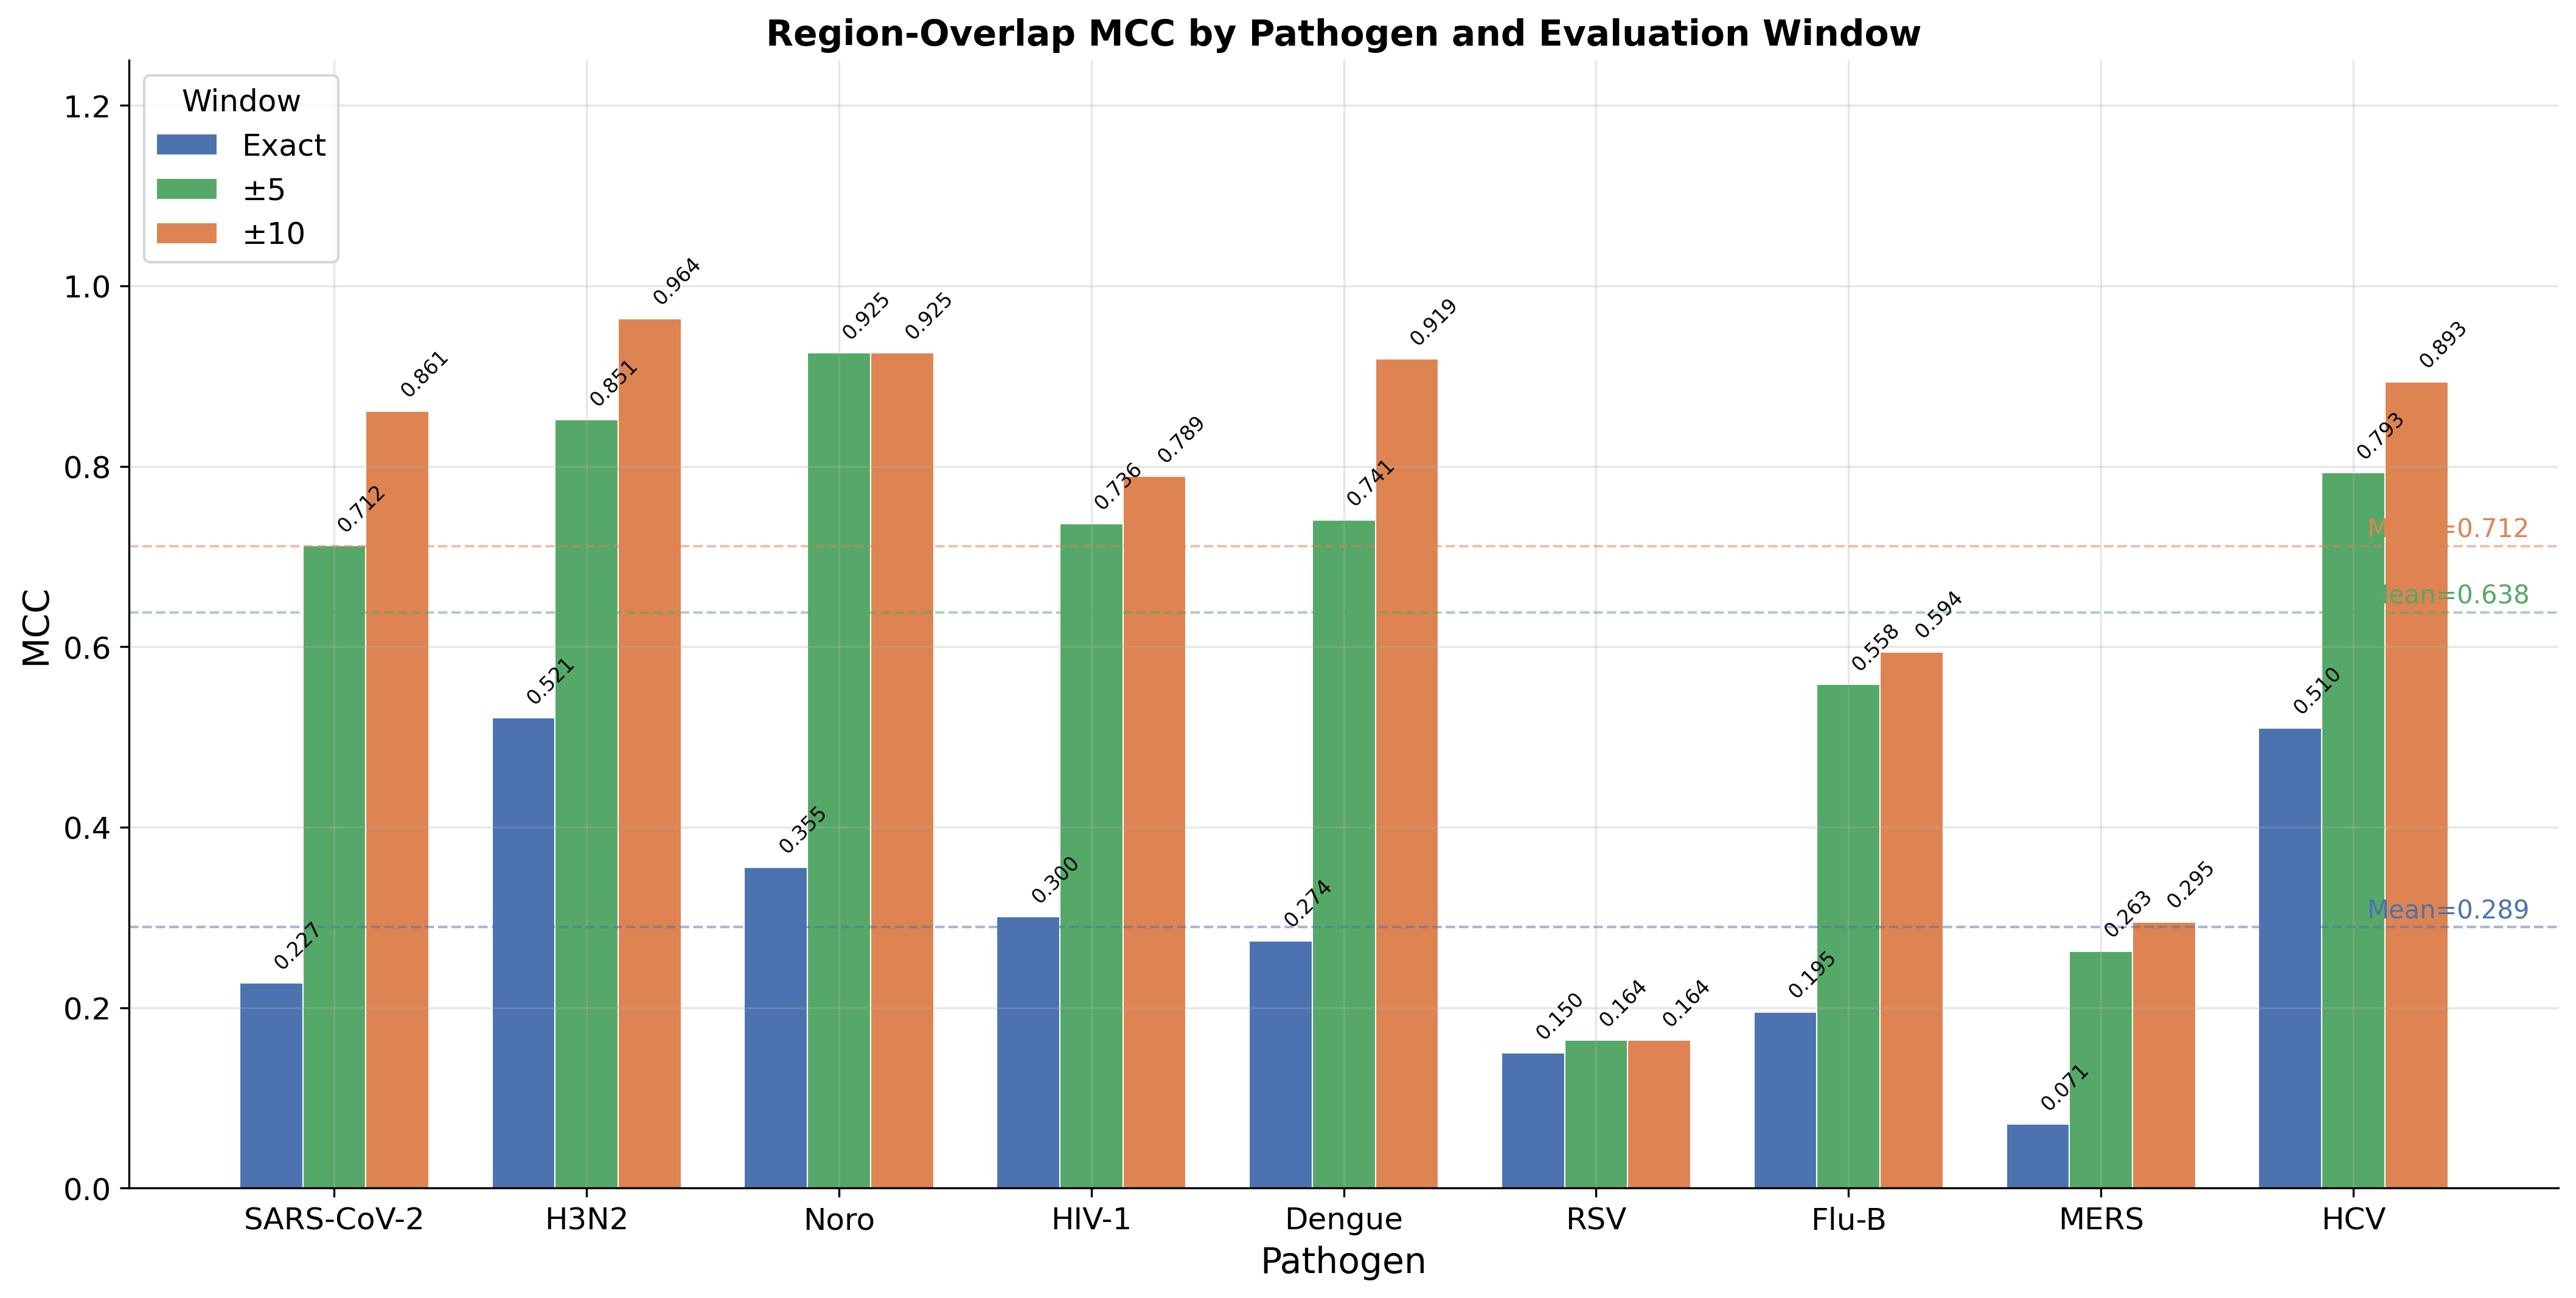
\includegraphics[width=\textwidth]{region_overlap_bar.png}
\caption{각 병원체에 대한 세 가지 평가 모드(정확 매칭, $\pm$5, $\pm$10 윈도우)에서의 영역 중첩 MCC. 정확 매칭에서 $\pm$10 윈도우 평가로의 일관된 향상은 탐지된 핫스팟이 9개 병원체 전체에서 ground truth 위치에 공간적으로 근접함을 보여준다.}
\label{fig:region_overlap_bar}
\end{figure}

Ground truth가 잘 특성화된 병원체에서는 실질적으로 높은 값을 달성한다.
이러한 상한 효과에도 불구하고, 벤치마크 결과는 공중보건 감시에 대한 실용적 함의를 가진다.

%% ============================================================
\section{실용적 함의와 근본적 한계}

제~\ref{ch:introduction}장에서 제기한 세 가지 문제로 돌아가면: 표준화된 평가 프레임워크의 부재는 MutBench의 3계층 ground truth와 hotspot-score 지표로 해결되었으며(기여 1); 교차 병원체 일반화 근거의 부족은 네 가지 독립적인 통계적 증거에 의해 해소되었고(기여 2); 탐지 방법의 병원체 의존성은 ANOVA 상호작용 우세($\omega^2 = 0.285$)와 LOPO 실패(0/9)로 정량화되어, PAHD 프레임워크의 동기를 제공하였다.

%% ============================================================
\subsection{공중보건 감시에서의 실용적 고려}
\label{sec:practical_surveillance}

SARS-CoV-2의 세대 시간(약 5일)과 서열 제출 지연(중앙값 약 14일)을 감안하면, 실시간 TC-freq 경보에는 최소 4주 윈도우가 필요하다.
조기경보에는 HDBSCAN-Auto(높은 재현율), 백신 후보 선정에는 MutClust-Hybrid(균형 성능)가 적합하며, 회고적 분석에서 MutClust-Hybrid의 높은 재현율은 신흥 핫스팟 위치의 조기 탐지 가능성을 시사하나, 정량적 시점 추정에는 별도의 시간적 검증이 필요하다.

2단계 탐지 파이프라인---HDBSCAN-Auto 1차 선별 후 MutClust-Hybrid 2차 확정(절~\ref{sec:variant_comparison})---은 정밀도(0.968)를 유지하면서 안정성이 0.740으로 향상되어 최고 hotspot-score(0.784)를 달성하였다.

\begin{table}[htbp]
\centering
\caption{2단계 파이프라인 검증 결과 (합성 데이터, 29,903 위치, 1,251개 ground truth 위치)}
\label{tab:twostep_pipeline}
\small
\begin{tabular}{lrrrrrr}
\toprule
\textbf{접근법} & \textbf{정밀도} & \textbf{재현율} & \textbf{F1} & \textbf{탐지 수} & \textbf{안정성} & \textbf{HS} \\
\midrule
HDBSCAN-Auto (단독) & 0.079 & 0.944 & 0.146 & 14,916 & 0.788 & 0.604 \\
MutClust-Hybrid (단독) & 0.968 & 0.659 & 0.785 & 852 & 0.706 & 0.778 \\
\midrule
\textbf{2단계 교집합} & \textbf{0.968} & 0.643 & 0.772 & 831 & \textbf{0.740} & \textbf{0.784} \\
\bottomrule
\end{tabular}
\end{table}

백신 설계 등 후속 실험 비용이 높은 응용에서는 이 2단계 접근법이, 일상 감시에는 MutClust-Hybrid 단독이, 조기경보에는 HDBSCAN-Auto 단독이 각각 적합하다.
다만, 실제 GISAID 2020--2021 데이터에서는 HDBSCAN-Auto가 비영 위치의 희소성(342개)으로 인해 클러스터를 형성하지 못하여, 2단계 파이프라인의 이점이 발현되지 않았다.
모든 빈도 기반 접근법에 영향을 미치는 근본적인 방법론적 한계는 계통발생 비독립성이다.

%% ============================================================
\subsection{계통발생 비독립성과 확장성 한계}
\label{sec:phylo_limits}

본 연구의 모든 탐지 방법은 서열 간 독립성을 암묵적으로 가정하나, SARS-CoV-2 서열은 계통발생적으로 구조화되어 있어 빈도 기반 접근법만으로는 양성 선택과 founder effect를 구분할 수 없다(예: D614G;~\cite{korber2020tracking}).
dN/dS 필터는 이를 부분적으로 해소하나, dN/dS 자체도 계통 구조에 의해 편향될 수 있다.

개념 증명 시뮬레이션(제~\ref{subsec:phylo_correction_poc}절)에서 Fitch 절약법 기반 homoplasy 점수가 수렴 변이를 정확히 최상위로 배치하였으며, TreeTime ML 확장 검증(제~\ref{subsec:treetime_ml_validation}절)에서 동등한 정확도(AUC = 1.000)를 확인하였다.
실제 GISAID 서열에 대한 경험적 검증(제~\ref{subsec:treetime_gisaid_validation}절)에서 H-score와 homoplasy 점수가 근본적으로 다른 신호를 포착함을 확인하여($\rho = -0.107$, $p = 1.36 \times 10^{-4}$), homoplasy 기반 보정의 실용적 가치를 뒷받침하였다.
Homoplasy 민감도 분석(제~\ref{subsec:homoplasy_sensitivity}절)은 2020-H1 서열 데이터와 Layer~A 수렴 진화 ground truth 간의 시간적 불일치를 드러내어, 계통발생 보정에는 시간적으로 정렬된 데이터가 필요함을 확인하였다.
완전한 계통발생 보정과 시간적으로 적절한 서열 표본 추출의 파이프라인 통합은 향후 핵심 확장 과제로 남아 있다(제~\ref{ch:conclusion}장).

%% ============================================================
\subsection{GISAID 데이터의 대표성과 표본 편향}

GISAID~\cite{shu2017gisaid} 기반 입력 데이터에는 체계적 편향이 존재한다.
\textbf{지리적 편향}: 고소득 국가가 전체 서열의 80\% 이상을 기여하여~\cite{chen2022gisaid}, 아프리카/남아시아의 고유 변이가 과소 반영되며, 주별 층화는 시간적 불균형만 보정한다.
\textbf{시간적 편향}: 초기 팬데믹과 Omicron 시기의 서열 축적량 차이가 크며, 주 내 대표성은 보장되지 않는다.
\textbf{Founder effect}: JN.1 확산에 동반된 ``hitchhiker'' 변이~\cite{kaku2024virological}처럼, 기능적 이점 없이 고빈도에 도달하는 위치를 양성 선택과 구분하는 것은 빈도 기반 접근법의 근본적 한계이다.

%% ============================================================
\subsection{범위 정당화: 9개 RNA 바이러스}

9종 병원체는 6개 주요 RNA 바이러스 과(Coronaviridae, Orthomyxoviridae, Retroviridae, Pneumoviridae, Flaviviridae, Caliciviridae)를 체계적으로 포괄하도록 선정되었으며, 팬데믹 잠재력을 가진 RNA 바이러스의 주요 분류학적 다양성을 대표한다.
RNA 바이러스로의 범위 제한은 의도적인 설계 결정이다: H-score 기반 스코어링은 충분한 변이 밀도를 요구하며, RNA 바이러스는 높은 변이율($10^{-3}$--$10^{-5}$ substitutions/site/year)로 이를 제공하는 반면, DNA 바이러스($10^{-6}$--$10^{-8}$)는 근본적으로 다른 스코어링 접근법을 필요로 한다.
표본 크기($n=9$)의 제한에도 불구하고, Friedman 검정은 $p=0.0015$를 달성하여, 효과 크기가 제한된 수의 병원체로도 탐지 가능할 만큼 충분히 크다는 것을 보여준다.

%% ============================================================
\subsection{ESM-2 학습 데이터 중복}
\label{sec:esm2_leakage}

ESM-2~\cite{lin2023esm2}는 바이러스 단백질 서열을 포함하는 UniRef50/UniRef90으로 학습되었으며, 본 벤치마크의 9개 대상 단백질(예: SARS-CoV-2 Spike, HIV-1 gp120, H3N2 HA)은 학습 코퍼스에 포함되어 있을 가능성이 높다.
따라서 ESM-2 log-likelihood ratio(LLR) 점수는 순수한 일반화 가능한 단백질 언어 이해가 아닌 기억된 진화적 패턴을 부분적으로 반영할 수 있으며, 이는 절대 AUC 값을 상향 편향시킬 수 있다.
그러나 이 우려는 분석의 9개 병원체 모두에 동일하게 적용되므로, 절대 성능 수준은 편향될 수 있으나 본 연구의 주요 발견인 교차 병원체 간 상대적 비교의 타당성은 유지된다.
의미 변화 특성(야생형과 돌연변이 임베딩 간 코사인 거리)은 절대 우도가 아닌 상대적 임베딩 변화를 측정하므로 학습 데이터 기억 효과에 대해 더 강건하다.
향후 바이러스 서열을 제외한 데이터베이스로 학습된 단백질 언어 모델을 평가하여 이 잠재적 편향의 크기를 정량화할 필요가 있다.

%% ============================================================
\subsection{병원체 간 Ground Truth 이질성}
\label{sec:gt_heterogeneity}

3계층 ground truth 프레임워크의 핵심 한계는 Layer~A(양성 선택 부위)가 병원체별로 정의되는 방식의 이질성이다.
SARS-CoV-2와 H3N2의 경우, Layer~A 위치는 계통발생적으로 확인된 수렴 진화 부위---동일한 돌연변이가 독립적으로 여러 계통에서 발생한 위치---이다.
반면, HCV의 Layer~A는 수렴적이 아닌 다양화 선택을 보이는 초가변 영역(HVR1/HVR2)으로 구성되며, Norovirus의 Layer~A는 항원 전환 사건과 관련된 시대적 변이 위치로 구성되고, 나머지 병원체는 다양한 수준의 계통발생적 확인을 거친 문헌 보고 면역 회피 부위를 사용한다(표~\ref{tab:gt_positions}).
이러한 이질성은 ANOVA에서 방법 $\times$ 병원체 상호작용을 인위적으로 부풀릴 수 있다. 병원체 생물학의 차이뿐만 아니라 ground truth 정의 기준의 차이도 관찰된 상호작용 효과($\omega^2 = 0.285$)에 기여할 수 있기 때문이다.
그러나 이 이질성은 핫스팟 탐지의 현실적 도전을 반영한다: ground truth 정의는 필연적으로 병원체별 생물학에 의존하며, 단일 기준(예: 수렴 진화만)으로는 모든 병원체에 적용할 수 없다.
탐지 성능이 병원체에 의존한다는 발견은 이 의존성이 병원체 간 본질적 생물학적 차이에서 비롯되든, ground truth 구성의 차이에서 비롯되든, 또는 양자의 상호작용에서 비롯되든 관계없이 유효하다---모든 경우에 실용적 함의는 동일하다: 단일 탐지 방법을 병원체 전체에 균일하게 적용하면 성능 저하가 발생한다.
또한, HCV는 유효 Layer~B 크기가 0이다(보존 영역이 정렬 길이 내에서 매핑될 수 없었음). 이는 HCV 평가가 Layer~A에만 의존함을 의미하며, HCV 특이적 결과를 해석할 때 이 비대칭성을 고려해야 한다.


% Chapter 6: Conclusion
\chapter{결론}
\label{ch:conclusion}

본 장에서는 MutBench의 학술적 기여를 요약하고, 한계점을 분석하며, 향후 연구 방향을 제시한다.

\section{연구 기여 요약}
\label{sec:contribution_summary}

본 학위논문은 바이러스 변이 hotspot 검출을 위한 체계적 벤치마킹 프레임워크인 MutBench를 제시하였다.
MutBench의 학술적 기여는 다음 두 가지로 요약된다.

\textbf{기여 1. MutBench 벤치마크 프레임워크.}
MutBench는 바이러스 변이 hotspot 검출 분야에 최초의 체계적 벤치마킹 프레임워크를 도입하였다.
수렴 진화 위치를 양성 기준(Layer~A), 정제 선택 위치를 음성 기준(Layer~B), DMS 실험 데이터를 기능적 적합도 기준(Layer~C)으로 활용하는 3계층 ground truth 체계를 정의하여, 기존의 자기 참조적 검증을 정량적이고 재현 가능한 비교로 대체하였다.
정확도(recall, precision)와 신뢰성(stability)을 동시에 평가하는 hotspot-score 복합 지표를 도입하고, 2단계 실험 설계를 통해 합성 데이터의 통제된 환경(1단계)과 9종 RNA 바이러스 대규모 비교(2단계)를 결합하여, 무작위 기준선 대비 통계적으로 유의한 탐지 성능을 확인하였다(상세 통계는 제~\ref{ch:results}장 참조).

\textbf{기여 2. 병원체 적응적 방법 선택 필요성의 통계적 입증.}
9종 RNA 바이러스에 대한 대규모 벤치마크 결과를 통계적으로 분석한 결과, 단일 최적 방법이라는 전제가 성립하지 않음을 네 가지 독립적 증거로 확립하였다.
첫째, ANOVA에서 방법 계열과 병원체 간 상호작용이 최대 분산 원천이었다.
둘째, 9개 병원체 모두 고유한 최적 scoring--detection 조합을 보였다(9/9 고유 최적 조합).
셋째, Friedman 검정은 방법 간 성능 순위가 병원체에 따라 체계적으로 달라짐을 확인하였다.
넷째, Leave-One-Pathogen-Out(LOPO) 교차 검증에서 0/9 일치로, 훈련 병원체에서 선택한 최적 조합이 새로운 병원체에 일반화되지 않았다.
이 결과는 병원체 적응적 방법 선택의 통계적 근거를 제공한다.
벤치마크 발견의 개념 증명 응용으로서, PAHD 프로토타입(제~\ref{subsec:pahd_prototype}절)은 게놈 프로파일 유사도가 탐지 패밀리 선호도를 부분적으로 예측할 수 있음을 보여주었다: v1 프로파일(8개 특성)은 5/9 양성 MCC, 중위수 MCC $= 0.014$(naive 중위수 $= 0.000$ 대비)를 달성하였고, v2 프로파일(85개 MSA 유래 특성)은 병리적 음의 전이를 제거하여 평균 MCC를 0.005에서 0.017로 개선하였다. 이는 벤치마크 결과가 실용적 방법 선택을 안내할 수 있음을 보여준다(상세 통계는 제~\ref{ch:results}장 참조).

MutBench의 체계적 벤치마킹 철학은 선행 연구인 MOSD~\cite{han2025mosd}에서 확립된 평가 원리를 바이러스 유전체학으로 확장한 것이다.

\section{한계점}
\label{sec:limitations}

\begin{table}[htbp]
\centering
\caption{MutBench 한계점 요약 및 완화 현황}
\label{tab:limitations_summary}
\small
\adjustbox{max width=\textwidth}{
\begin{tabular}{llll}
\toprule
\textbf{한계점} & \textbf{심각도} & \textbf{현재 완화} & \textbf{향후 연구} \\
\midrule
Ground truth가 문헌에 한정 & 높음 & DMS 검증 포함 3계층 GT & 추가 병원체 확대 \\
DMS 데이터 4/9 병원체만 확보 & 중간 & 나머지 5종 Layer A+B 사용 & 신규 DMS 실험 \\
계통발생 비독립성 & 높음 & PoC 시뮬레이션 ($\rho=-0.876$) & TreeTime 파이프라인 통합 \\
합성--실제 데이터 성능 격차 & 중간 & 이중 벤치마크 설계 & 적응적 참조 서열 \\
위치 수준 정확 매칭 & 중간 & 농축비 보완 & 영역 중첩 지표 \\
RNA 바이러스만 (9종) & 낮음 & 주요 RNA 과 포괄 & DNA 바이러스 확장 \\
GISAID 표본 편향 & 중간 & 주별 시간적 층화 & 지리적 층화 \\
\bottomrule
\end{tabular}
}
\end{table}

\subsection{Ground truth 한계}

MutBench의 3계층 ground truth는 현재 SARS-CoV-2에 한정되어 정의되어 있다.
Layer~C(DMS 기능적 적합도)는 Dadonaite 등~\cite{dadonaite2023dms}의 전체 Spike DMS 데이터에 기반하므로, DMS 데이터가 확보되지 않은 병원체에는 Layer~A(수렴 진화)와 Layer~B(정제 선택)만 적용 가능하다.
또한 DMS 데이터 해석 시 기능적으로 중요한 위치를 정의하는 임계값(예: fitness effect $\leq -0.5$)의 선택이 ground truth의 구성에 직접 영향을 미치므로, 해당 임계값에 대한 민감도가 존재한다.
DMS는 유사바이러스 시스템을 사용한 시험관 내(in vitro) 분자 적합도를 측정하므로, 생체 내(in vivo) 적합도를 완전히 포착하지 못할 수 있다.

\subsection{계통발생 비독립성}

H-score는 변이 빈도에 기반하므로, 계통발생학적 구조에 의한 교란에 취약하다.
D614G와 같은 고빈도 변이는 독립적인 양성 선택이 아닌 단일 창시자 효과(founder effect)에서 기인할 수 있으며($\rho = -0.876$, H-score와 독립적 변이 발생 횟수 간 Spearman 상관), GISAID의 시퀀싱 편향(특정 국가 및 시기의 과대 대표)은 변이 빈도 분포를 왜곡한다.
MutBench는 합성 H-score와 DMS 기반 ground truth를 사용함으로써 이 문제를 부분적으로 완화하나, 실제 데이터에의 적용을 위해서는 계통발생학적 보정이 필수적이다.

\subsection{범위 한계}

9종 RNA 바이러스(SARS-CoV-2, Influenza A/B, HIV-1, RSV, Dengue, HCV, MERS-CoV, Norovirus)에 대한 평가를 수행하였으나, DNA 바이러스(HPV, HBV 등)의 상이한 변이 메커니즘에 대한 검증은 아직 수행되지 않았다.
또한 MutBench의 현재 구현은 점 변이(point mutation)만을 대상으로 하며, 삽입/결실(indel)은 배제되어 있다.
단백질 언어 모델(ESM-2 등)을 활용한 위치별 적합도 예측의 통합 역시 향후 과제로 남아 있다.

\subsection{합성 데이터와 실제 데이터 간의 격차}

1단계 합성 벤치마크에서의 성능(hotspot-score 0.778)과 GISAID 실제 데이터에서의 성능 간에는 격차가 존재한다.
실제 H-score의 희소 분포(29,903개 위치 중 342개만 비영)는 합성 벤치마크의 연속적 배경 잡음과 질적으로 상이하다.
다만 모든 방법의 농축비가 7배 이상을 유지하여, 탐지의 생물학적 타당성은 데이터 유형에 관계없이 보존되었다.

\subsection{위치 수준 평가의 한계}

MutBench의 precision과 recall은 정확한 뉴클레오티드 위치 수준에서 계산되므로, ground truth에서 단 한 위치만 벗어난 검출도 위양성(false positive)으로 분류된다.
윈도우 기반 또는 영역 중첩 지표가 검출의 실용적 유용성을 보다 관대하게 반영할 수 있다.

\section{향후 연구 방향}
\label{sec:future_work}

\begin{table}[htbp]
\centering
\caption{우선순위별 향후 연구 로드맵}
\label{tab:future_roadmap}
\small
\adjustbox{max width=\textwidth}{
\begin{tabular}{llll}
\toprule
\textbf{우선순위} & \textbf{연구 방향} & \textbf{선결 조건} & \textbf{기대 영향} \\
\midrule
1 (최고) & 계통발생 보정 통합 & TreeTime 파이프라인 & Founder effect 편향 해소 \\
2 & PAHD 구현 & 보정된 벤치마크 데이터 & 적응적 방법 선택 \\
3 & DNA 바이러스 확장 & 신규 ground truth 구축 & 적용 범위 확대 \\
4 & 실시간 감시 통합 & 점진적 H-score 업데이트 & 공중보건 실용성 \\
\bottomrule
\end{tabular}
}
\end{table}

\subsection{PAHD: 벤치마크 응용에서 완전한 구현으로}

제~\ref{subsec:pahd_prototype}절에서 제시한 PAHD 프로토타입은 벤치마크 결과의 개념 증명 응용으로 기능하며, MutBench의 통계적 발견(기여 2)이 실용적 방법 선택 전략으로 전환될 수 있음을 보여준다.
두 가지 프로파일 버전을 평가하였다: v1(8개 메타데이터 특성)과 v2(스코어링별 통계량, 교차 점수 상관, 공간적 자기상관을 포함한 85개 MSA 유래 특성).
v1 Family-first 전략은 5/9 양성 MCC, 중위수 MCC $= 0.014$(naive 중위수 $= 0.000$ 대비)를 달성하였고; v2 프로파일은 더 판별적인 병원체 유사도 점수를 통해 병리적 음의 전이를 제거하여(예: HCV $-0.291 \rightarrow +0.141$) 평균 MCC를 0.005에서 0.017로 개선하였다.
그러나 정확 일치율은 v1과 v2 모두에서 0/9로 유지되어, 85개 특성을 사용하더라도 $n = 9$ 병원체의 근본적 한계가 지속됨을 확인하였다.
더 거친 예측 단위---탐지 패밀리(15개 패밀리)와 스코어링 공식(9개 공식)---에서 평가할 때, 일치율은 역시 0/9이었으나 달성된 MCC는 실질적으로 개선되었다: 패밀리 수준 예측은 oracle 성능의 49.2\%(평균 MCC $= 0.144$)를, 스코어링 수준 예측은 54.5\%(평균 MCC $= 0.172$)를 회복하여, 정확한 조합 예측(oracle의 $-9.8$\%)을 크게 능가하였다.
이는 라벨 예측이 실패하더라도 거친 단위에서의 예측이 경쟁력 있는 탐지 성능을 산출함을 보여주며, knowledge base 확대에 따른 계층적 예측 접근법의 타당성을 뒷받침한다.
병원체 수를 20개 이상으로 확대하고, 상위 $k$개 앙상블 전략을 도입하며, 메타학습 회귀 모델~\cite{rice1976algorithm,smith2021algorithm}로 전환하는 것이 완전한 PAHD 구현을 위한 구체적 후속 단계이다.

\subsection{계통발생학적 보정 통합}

제~\ref{sec:phylo_simulation}절에서 보고된 개념 증명 결과는 homoplasy 기반 스코어링이 빈도 기반 H-score와 질적으로 다른 진화적 신호를 포착함을 확립하였다: coalescent 시뮬레이션에서 $\rho = -0.876$, TreeTime ML 조상 재구성($N = 2{,}000$)에서 AUC $= 1.000$, 실제 GISAID 서열($N = 500$)에서 $\rho = -0.107$.
구체적인 통합 경로로서, H-score를 조상 재구성에 의해 추론된 독립적 변이 발생 횟수인 homoplasy count로 대체하여 스코어링 공식의 입력으로 사용하며, 이를 위해 각 병원체에 대해 TreeTime~\cite{sagulenko2018treetime} 조상 재구성을 전처리 단계로 수행해야 한다.
주요 계산 병목은 TreeTime의 서열 수에 대한 $O(N \log N)$ 스케일링이나, UShER~\cite{turakhia2020ultrafast} 등 최신 초고속 대안은 수백만 서열 처리를 가능케 하여 GISAID 규모에서의 통합이 실현 가능하다.
계통발생학적 보정은 주로 강한 창시자 효과를 가진 병원체에 영향을 미칠 것이며(예: SARS-CoV-2 D614G, H-score 순위 2위이나 homoplasy 순위 1,134위), 해당 병원체의 최적 스코어링--탐지 조합을 변경하고 전체 oracle MCC를 개선할 가능성이 있다.
시기별 서열 비율을 정규화하는 시간적 층화(temporal stratification)는 트리 위상과 독립적으로 시퀀싱 편향을 완화하여 계통발생학적 보정을 보완할 것이다.

\subsection{DNA 바이러스 확장}

HPV, HBV 등 DNA 바이러스로의 확장은 MutBench 프레임워크의 일반화 범위를 검증하는 핵심 과제이다.
DNA 바이러스는 RNA 바이러스에 비해 낮은 변이율과 상이한 변이 메커니즘(예: APOBEC3 매개 탈아미노)을 가지므로, 현재의 스코어링 및 탐지 방법이 동일하게 적용 가능한지 검증이 필요하다.

\subsection{Indel 및 단백질 언어 모델 통합}

현재 배제된 삽입/결실(indel)을 H-score 프레임워크에 통합하기 위한 gap 처리 전략의 개발이 필요하다.
또한 단백질 언어 모델(ESM-2/ESM-3)의 로그 우도비를 위치별 적합도 점수로 활용하여, H-score의 해석 가능성과 딥러닝의 패턴 학습 능력을 결합하는 다중 스케일 점수 체계가 구상된다.

\subsection{실시간 감시 체계 연동}

장기적으로는 MutBench에서 검증된 최적 탐지 방법을 실시간 유전체 감시 파이프라인에 통합하는 것이 목표이다.
이는 스트리밍 시퀀싱 데이터에 대한 점진적 H-score 업데이트, 신규 변이체 출현 시 자동 경고, 하수 감시 데이터와의 통합을 포함한다.
MutBench의 stability 지표는 이러한 실시간 응용에서 검출 결과의 신뢰성을 보장하는 데 핵심적인 역할을 한다.

\section{맺음말}
\label{sec:final_conclusion}

COVID-19 팬데믹은 바이러스 변이 핫스팟 탐지가 단순한 학술적 작업이 아니라 공중보건의 필수 과제임을 드러내었다.
본 학위논문은 바이러스 변이 hotspot 검출을 위한 최초의 체계적 벤치마킹 프레임워크인 MutBench를 제시하고, 9종 RNA 바이러스에 대한 대규모 벤치마크 평가(총 3,321개 평가, 통계 검정에는 비영 MCC 2,544개 사용)를 통해 단일 최적 방법이 존재하지 않음을 통계적으로 입증하였다.
MutBench 이전에는, 핫스팟 탐지 방법을 적용하는 연구자가 방법 선택에 대한 정량적 근거를 가지고 있지 않았다; MutBench는 표준화된 ground truth, 복합 평가 지표, 교차 병원체 통계적 증거를 통해 이 근거를 제공한다.
이 결과는 병원체 특성에 기반한 적응적 방법 선택이 필수적임을 확립한다; PAHD 프로토타입(v1 및 v2 프로파일)은 이 발견의 개념 증명 응용이며, v2 MSA 유래 프로파일은 개선된 유사도 보정을 보여주었으나, $n = 9$ knowledge base 한계는 더 많은 병원체로의 확대가 핵심 후속 단계임을 확인한다.
탐지 방법 성능이 방법 자체가 아닌 방법--병원체 상호작용($\omega^2 = 0.285$)에 의해 지배된다는 발견은 바이러스 유전체학을 넘어 더 넓은 함의를 가진다: 이질적인 입력 분포에 걸쳐 알고리즘이 적용되는 모든 도메인에서, 숨겨진 상호작용 효과를 노출하고 원칙적인 알고리즘 선택을 안내하기 위한 유사한 체계적 벤치마킹이 유익할 수 있다.
MutBench에서 확립한 3계층 ground truth, hotspot-score 복합 지표, 그리고 대규모 벤치마크 결과는 바이러스 유전체 감시와 변이체 대응 연구의 정량적 기반을 제공한다.

\section*{코드 및 데이터 가용성}

MutBench 프레임워크의 소스 코드, 벤치마크 스크립트, 9종 병원체별 ground truth 정의, 그리고 모든 실험 결과의 재현에 필요한 설정 파일은 GitHub 저장소(\url{https://github.com/hwijun/mutbench})에서 공개될 예정이다.
모든 저장소는 학위논문 심사 완료 후 공개된다.
병원체 서열 데이터는 NCBI GenBank에서 수집하였으며, SARS-CoV-2 DMS 데이터는 Dadonaite 등~\cite{dadonaite2023dms}에서 제공된 원본 데이터를 사용하였다.


%% ----------------------------------------------------------
%% 후면부 (Back Matter)
%% ----------------------------------------------------------

%% 참고문헌
\bibliography{references}

%% 영문 초록
\makeengabstract{%
  % Abstract
This dissertation presents \textbf{MutBench}, a hotspot-detection benchmark that systematically compares 10 biological information types (20 scoring formulas) $\times$ 14 detection families (39 variants) $\times$ 11 RNA viruses = 8{,}580 evaluations. The headline result: the optimal information source is pathogen-dependent, with the scoring~$\times$~pathogen interaction ($\omega^2 = 0.296$, 11-pathogen cluster-bootstrap 95\% interval [0.195, 0.333]) as the largest modeled variance component, and HIV-1 vaccine-escape enrichment of $7.19\times$ (Bonferroni $p = 2.5 \times 10^{-16}$) as the primary external anchor.

Detecting mutation hotspots in viral genomes is essential for variant surveillance and vaccine design, yet existing approaches have relied almost exclusively on mutation frequency and Shannon entropy, leaving comparatively unexplored a rich landscape of complementary information sources (phylogenetic selection signals, protein language models, structural features). Concurrent fitness-regression benchmarks (ViroGym, EVEREST~v3, ProteinGym~v1.3) target per-variant prediction; MutBench is the broadest \emph{region-level hotspot-detection} benchmark to date.
MutBench comprises three core components:
(1) a three-layer ground truth system integrating literature-curated positive markers (Layer~A: a pathogen-specific union of convergent-evolution, immune-escape, and HVR-membership evidence types, with immune-escape positions dominating the curated set), conserved structural regions under purifying selection as negative controls (Layer~B), and Deep Mutational Scanning (DMS) experimental fitness data as functional validation (Layer~C);
(2) a composite evaluation metric defined as $\text{hotspot-score} = (\text{recall} + \text{precision} + \text{stability}) / 3$; and
(3) a two-stage experimental design in which Stage~1 conducts in-depth analysis on SARS-CoV-2 and Stage~2 performs the large-scale cross-pathogen comparison.

Stage~1 validates the framework on SARS-CoV-2 (MutClust-Hybrid hotspot-score 0.778). Stage~2 establishes that the optimal information source varies systematically across pathogens: $\omega^2_{\text{scoring}\times\text{pathogen}} = 0.296$ (11-pathogen cluster-bootstrap 95\% interval [0.195, 0.333]; 6-category aggregation gives $\omega^2 = 0.103$ as a collinearity-robust lower bound; within-cell residual $\omega^2 \approx 0.39$). Friedman test shows no universally best combination ($\chi^2 = 7.69$, $p = 0.990$), and LOPO yields 0/11 exact matches with a 0.265 oracle-vs-generalized MCC gap (LOPO 0/11 alone is null-consistent under permutation; the conclusion rests on the interaction effect plus the vaccine-escape audit, not on LOPO in isolation).
Contribution 3 is two-part: \textit{(3a) Multi-source integration infrastructure} ---a 4-feature core captures $\approx$98\% (97.6\%) of the 10-feature ensemble; EqualWeight integration achieves H3N2 enrichment 4.012$\times$ ($p = 0.0023$). \textit{(3b) External validation, anchored on HIV-1} ---under a three-tier evidence rule (Bonferroni survival~$\times$~Layer~A overlap < 33\%), HIV-1 is the primary anchor with direct novel-only Fisher enrichment $7.16\text{--}8.24\times$ on the 37 Layer-A-disjoint positions (worst-case $p = 5 \times 10^{-12}$); H3N2 ($9.36\times$, 69\% overlap) is a self-consistency check; SARS-CoV-2 ($7.63\times$) is exploratory after Bonferroni. Validation is restricted to 3/11 pathogens (2{,}340 evaluations) by availability of curated antibody-escape annotations.

A systematic analysis of the 20 scoring types spanning six information categories (frequency, MSA-derived, phylogenetic, structural, AI-based, and composite) reveals 9 distinct optimal information types across 11 pathogens: FUBAR phylogenetic selection scores achieve the highest MCC for H3N2 (0.534), protein language model scores dominate for SARS-CoV-2 and RSV, and homoplasy scores excel for Norovirus.
Multi-source integration further reduces the experimental search space for hotspot validation, achieving 4.012$\times$ vaccine escape enrichment for H3N2 ($p = 0.0023$), while a compact 4-feature core captures $\approx$98\% (97.6\%) of full-ensemble performance.

\vspace{1em}
\noindent\textbf{Keywords}: mutation hotspot detection, MutBench, biological information types, viral genomics, multi-source information analysis, pathogen-dependent optimality, SARS-CoV-2, Deep Mutational Scanning

}

\end{document}
